\documentclass[11pt, oneside]{report}  
\usepackage{algorithm}
\usepackage{algorithmic}
% Theorem environments
\newtheorem{claim}{Claim}
\newtheorem{class}{Class}
\newtheorem{definition}{Definition}
\newtheorem{example}{Use Case}
\newtheorem{observation}{Observation}
\newtheorem{property}{Property}
\newtheorem{proposition}{Proposition}
\newtheorem{theorem}{Theorem}

% font
%\usepackage{helvet}
%\renewcommand{\familydefault}{\sfdefault}
\usepackage{sectsty}
\allsectionsfont{\sffamily}

% end Theorem environments
\usepackage{amssymb}
\usepackage{amsmath}
\usepackage{color}
\usepackage{enumitem}
\usepackage[T1]{fontenc}
\usepackage[multiple]{footmisc}
\usepackage[top=1.5in,bottom=1.5in,left=1.30in,right=1.30in]{geometry}
\usepackage{graphicx}	
\usepackage{ifpdf}
\usepackage{listings}
\usepackage{multirow}
\usepackage[normalem]{ulem}
\usepackage{soul}
\usepackage{subfigure}
\usepackage{txfonts}
\usepackage{times}
\usepackage{url}

% MARCOS PARAGRAPH SEPARATION:
\setlength{\parindent}{0px}
\setlength{\parskip}{1em}
% Glossy
\newif\ifpdf
\ifx\pdfoutput\undefined
  \pdffalse
  \usepackage[colorlinks=false]{hyperref}
\else
  \pdfoutput=1
  \pdftrue
  \usepackage[pdftex,colorlinks=false,urlcolor=blue,linkcolor=blue]{hyperref}
  \pdfcompresslevel=9
  \usepackage{pslatex}
\fi
\newcommand{\mathendbox}{\hfill$\Box$}
\newcommand{\minisec}[1]{\noindent\textbf{#1.}}
\newcommand{\denote}[1]{\text{$[\![ $#1$ ]\!]$}}
\newcommand{\opsem}[3]{\text{$<$#1,#2$>\Downarrow$#3}}
%%%%%%%%%%%%
% MVS: Language definitions
%
\renewcommand{\ttdefault}{pcr}
\lstset{
  basicstyle=\small\ttfamily,
  breaklines=true
}
\lstdefinelanguage{sql}{
  morekeywords={SELECT, FROM, WHERE, ITERATE, RECURSE, OVER, IN, RANGE, FROM, TO, SEQUENCE, FOREACH, PAIR, LOCUS, ID, MAP, FILTER, LIMIT, SCALE,LINEAR,LOG,WEIGH,BY,SUBJECT,TO,AND,AS, NOT, DROP, ONE, BOTH, WITH, RECURSIVE, UNION, ALL, PARTITION,ORDER,DESC,ASC,JOIN,ON,OR,GROUP,HAVING,BETWEEN,USING,EXISTS},
  sensitive=true,
  morecomment=[l]{//},
  morecomment=[s]{/*}{*/},
  morestring=[b]",
}
%\lstset{
%  language=sql
%}
\lstdefinelanguage{cvl}{
  morekeywords={geometry, id, generalize,to, with, other, at, zoom, levels, weigh, by, subject, and, create, constraint, as, not, exists, resolve, if, delete, select, from, where, in, order, over, setup, teardown,force,min,level,for,allornothing,join,on,setup,group,having,index,temporary,table,drop,partition,merge,partitions},
  sensitive=false,
  morecomment=[l]{//},
  morecomment=[s]{/*}{*/},
  morestring=[b]",
}
%\lstset{
%  language=cvl
%}

\newcommand{\nice}[1]{\ \\ \fbox{\parbox{1.0\linewidth}{{\sc Nice sentence}:\\ #1}}}

\newcommand{\todo}[1]{\ \\ \fbox{\parbox{1.0\linewidth}{{\sc TODO}:\\ #1}}}

\newcommand{\note}[1]{\ \\ \fbox{\parbox{1.0\linewidth}{{\sc Note}:\\ #1}}}

\newcommand{\marcos}[1]{\ \\ \fbox{\parbox{1.0\linewidth}{{\sc Marcos}:\\ #1}}}

\newcommand{\pitfall}[1]{\ \\ \fbox{\parbox{1.0\linewidth}{{\sc Pitfalls in Writing}:\\ #1}}}


\sloppy

\title{Geodata Visualization Management Systems}
%\title{Building Scalable Data Visualization Management Systems}
%\title{Declarative Selection for Multi-scale Visualizations Systems}
%\title{Selection Problems in Multi-scale Data Visualizations Systems}
%\title{Selection Problems in High-Performance Multi-scale Visualizations}
%\title{Data Selection in High-Performance Visualizations on the Web}
%\title{Selection Problems in High-Performance Data Visualizations for the Web}
%\title{Selection Problems in Data Visualizations for the Web}
%\title{Title to be decided}

\author{Pimin Konstantin Kefaloukos}
%\date{}							% Activate to display a given date or no date

\begin{document}
\maketitle

\section*{Acknowledgements}
First and foremost, I wish to dedicate this work to my son Morgan and my daughter Athena. Thank you for blessing my life with your love and magic. Thank you also to my ex-wife Marusa for being a wonderful co-parent to our children, a great support, and a source of life-long inspiration. Next, and with very deep gratitude, I wish to thank my primary supervisor Marcos Vaz Salles for his tireless dedication and support, the great discussions we had, and for his warm friendship. Furthermore, I wish thank my supervisor Martin Zachariasen, for always keeping a cool head, believing in my ideas and for giving me the right push whenever I needed it. With sincerity, I wish to thank the Ministry of Higher Education and Science in Denmark, Grontmij A/S and the Danish Geodata Agency, without whose financial support this industrial PhD thesis would not have materialized. In particular, I would like to thank Anders Friis-Christensen, Thorben Hansen and Nils Bo Wille-J{\"o}rgensen who are the people who took a chance and made it all possible. With a wam heart, I want to thank my father Georgios Kefaloukos, my mother Helena Hodgson and my step-father Stuart Hodgson for their great support and for always being proud of me. A special warm thought also goes out to Dora and Tonci Balic-Zunic, for many fond memories with the family and for being active grand parents when at times it was helpful. Another special thought goes out to the faculty at DIKU and all the PhD students, especially Vivek Shah, for fun and thought-provoking discussions over lunch in the cantine. It was sometimes silly and often enlightning. Also, I wish to thank Professor Robert Weibel who hosted me at the University of Z{\"u}rich (UZH), Department of Geography during my 3-month stay in Switzerland, as well as everybody in the department who offered their feedback, helped with accomodation, and sometimes invited me for cake and espresso. My talented colleagues at Grontmij A/S and the Danish Geodata Agency deserve a special thanks for their frequent and often pragmatic feedback on my work. I also reserve a special place in my heart for my friends, who forced me to go out and have some fun once in a while. As a commemoration, I would like to thank the late S{\o}ren Aundal, a primary school teacher who recently passed away. When I was a kid, he showed me how to train a pair of binoculars at birds, stars and planets in the sky, thus sparking my enduring curiosity about the world. Last but not least, I would like to thank Hans Skov-Petersen and Bernhard Snizek for kick starting my interest in the field of geographical data science, and by transitivity, in data science as a whole. Finally, I must acknowledge that I can never fully understand the influences that have lead me to this point. Instead, I close my eyes and humbly recognize that in the great labyrinth of human existence, I have never walked alone.

\tableofcontents

\abstract{Abstract goes here.}


%  ############
%  #  CHAPTER  
%  ############ 

\chapter{Introduction}
\label{chapter:introduction}

% \marcos{Regarding the chapters for the three papers: review the text, see if there are any arguments that can be improved; no time to redo non-text work.}
% \todo{Cite everything that is cited by The Case for Data Visualization Management Systems (33 citations)}

\note{Must have a section that clearly defines the problem I solve, the requirements for the system I propose, and my contributions toward solving this problem.}

\vspace{-4ex}
\section{Background and Motivation}
\label{sec:introduction:background:and:motivation}
% Maps are important
Map visualization studies how to visually represent the geography of the Earth at multiple scales (i.e. with pan and zoom) on restricted mediums, such as computer screens. Map visualization is a facet of the data visualization field, which is the study and creation of (interactive) visual representations of data to reinforce human cognition~\cite{friendly2008milestones}. However, the specific value proposition of geographical maps is clear: maps save lives~\cite{openstreetmap2010haiti}; maps crucially assist navigation~\cite{something}; maps increase the transparency and efficiency of our societies~\cite{gst2012friedata}. The human human mind has such a strong affinity for spatial reasoning that map metaphors are used to reason even about non-spatial phenomena~\cite{shahaf2013informationcartography, daniels2014vocabulary}.

Today, the web offers a huge diversity of curated~\cite{gst2014digitalmapsupply} and user-contributed~\cite{openstreetmap, zooniverse2014oldweather} datasets that can be visualized on maps. While geographical data is characterized by great diversity, is also reaches great volume. Each day, millions of new objects are added to the OpenStreetMap database that already contains billions of objects~\cite{openstreetmap2014stats}. Still, OpenStreetMap accounts for just a tiny fraction of all spatial data on the web, and perpaps, we have only seen the beginning. In 2014, a company launched a system of micro satellites equipped with multi-band sensors that will capture the entire surface of the Earth in high resolution every day~\cite{planetlabs2014flock1}. Moreover, as mobile devices increasingly bond millions of people to spatial services, such as dating~\cite{tinder2014tinder}, transportation~\cite{drivr2014drivr} and games~\cite{geocaching2014geocaching}, geographical information can be produced and consumed by anybody, anytime, and anywhere.

More and more, organizations with no strong tradition for geography (e.g. news agencies) communicate spatial narratives using maps~\cite{nytimes2010iraq}. As a consequence, more and more professionals will need to acquire the skills to craft map visualizations. One of the most crucial problems in map creation is the mismatch between data volume and the small representational budget of computer screens. For example, a laptop display (e.g. 2880 x 1800 pixels) can display just a few thousand symbols without overlap, which is entirely indadequate for displaying most geographical datasets. Necessarily, geographical data must be abstracted (e.g. filtered~\cite{} or aggregated~\cite{}) according to scale in order to produce a legible and useful map. However, filtering and aggregation for maps is much more complex than the similarly named operations in statistics. Within map visualization, the disciplin of map generalization studies how geographical data should be abstracted as the scale changes. In contrast to selection, projection and aggregation in the relation algebra, map generalization must select, project and aggregate data \emph{holistically} according to visual constraints and objectives~\cite{weibel1999generalising}.

% Why GIS is inadequate
Traditionally, maps have been crafted by experts in Geographical Information Systems (GIS). However, a new situation exists on the web today that significantly marginalizes the use for traditional GIS. First, the demand for multi-scale maps on the web is rising faster than the number of GIS experts who know how to craft them (using traditional GIS); therefore, map visualizations must be \emph{expressible by non-experts}. Second, web maps that run on top of cloud infrastructures can now integrate huge datasets (billions of data items); therefore, map visualization systems must be \emph{scalable in the size of data}. Third, web maps today can quickly reach millions of users who can interact with map visualization 24 x 7 using mobile devices; therefore, map visualization systems must be \emph{scalable in the number of concurrent users} and \emph{highly available}. In short, GIS was not designed to satisfy these requirements, which merits the study of a new category of systems.

To address the short-comings of GIS for the web, this dissertation makes the case for a new category of systems: Map Visualization Management Systems (MVMS). The vision of MVMS is influences by the visions of Reverse Data Management~\cite{meliou2011reverse} and Data Visualization Management Systems (DVMS), however specialized for the particular challenges of map visualization.

\emph{copy-pasted} While data can be both numerical and non-numerical, this thesis will focus on geographical data that is stored in tables, e.g. rows in an RDBMS. At first, this may seem constricted, however tables are versatile and make up the bulk of all data that is visualized today~\cite{wu2014case}.

\section{Challenges}
\label{introduction:challenges:in:map:visualization}

\begin{figure}[htbp]
\begin{center}
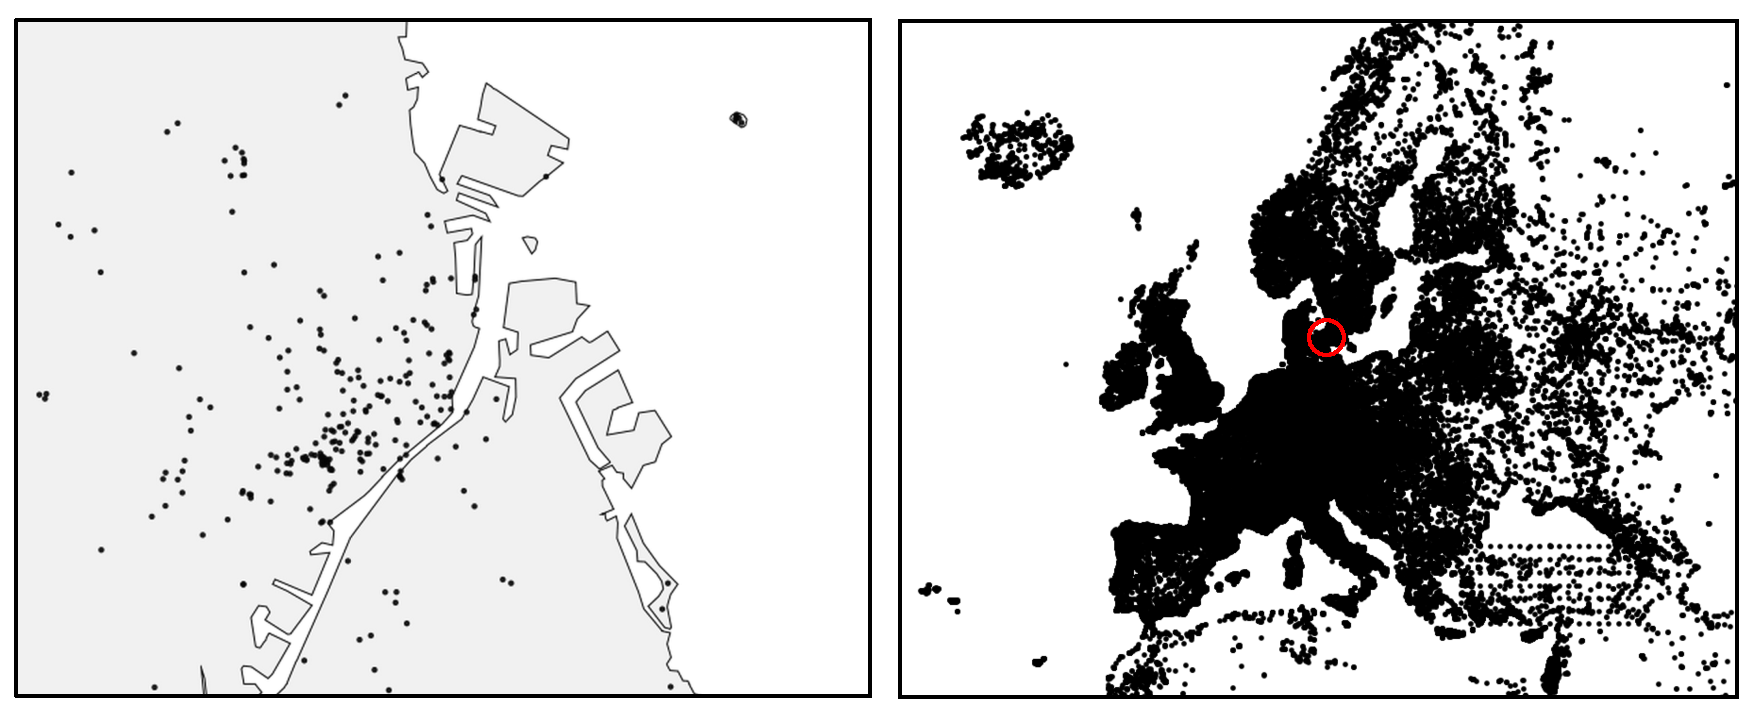
\includegraphics[scale=.5]{figs-thesis/data-draws-the-world.pdf}
\caption{\emph{Data vs territory:} On a low scale map of Europe, the 5 x 5 pixel data symbols for tourism points of interest (left map) more or less cover the national territories (right map). Thus, for large datasets (thousands of records) displaying unfiltered data symbols is non-sensical. First, users can not discrimiate between interesting data and less interesting data. Second, users can not orient themselves as crucial spatial context is lost when map labels are eclipsed by data symbols. Third, users can not accurately interact with the data symbols to get more information. For example, there are 28 thousand data points in the vicinity of Paris; which one is the Eiffel Tower?}
\label{default}
\end{center}
\vspace*{-4ex}
\end{figure}


Systems that address some, but not all 

Large organizations like Google and Microsoft can afford the development costs of creating 

\emph{What are the requirements?}
A map visualization must be \emph{scalable} both in the size of data~\cite{lins2013nanocubes, Im2013visreduce, battle2013scalar, liu2013immens} and the size of the audience~\cite{viegas2007manyeyes}. Todays users on the web expect acceptable latency for an application. Failure to recognize this condition will result in loss of users, which has been studied in the areas of search and e-commerce~\cite{google2010latency, amazon2010latency}

A map visualization must be \emph{expressible};

A map visualization must be \emph{available};

 Additionally, it is crucial that designers can craft visualizations using interfaces that are both intuitive, efficient (in terms of wall-clock time) and expressive (in terms of ). Crafting a map visualizationg involves a process of abstraction, including data abstraction and visual abstraction (see Figure~\ref{foo}).

\emph{What is special about geography?}

\begin{figure}[htbp]
\begin{center}
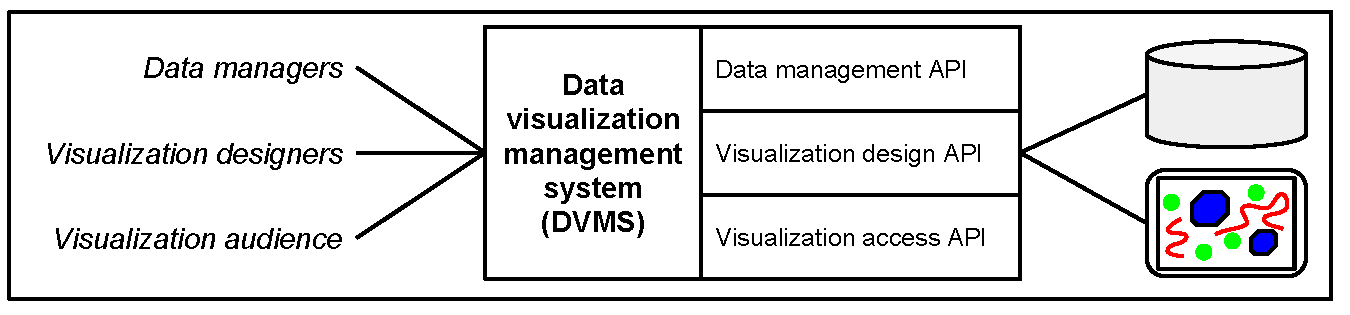
\includegraphics[scale=.6]{figs-thesis/data-visualization-management-system.pdf}
\caption{TODO}
\end{center}
%\vspace*{-4ex}
\end{figure}

% Requirements for new system: MVMS

% MOVE TO RELATED WORK
%Data Visualization Management Systems (DVMS) have been proposed as a solution for data-driven visualizations on the web today~\cite{wu2014case, fekete2012dmvis}. The API of a fully-fledged DVMS includes components for both data management, visualization design, and visualization sharing~\cite{foo}. A DVMS must be scalable both in the size of data~\cite{lins2013nanocubes, Im2013visreduce, battle2013scalar, liu2013immens} and audience~\cite{viegas2007manyeyes}. Additionally, it is crucial that designers can craft visualizations using an interface that is both intuitive, efficient (in terms of wall-clock time) and expressive. In the geographical domain, prototypes of such systems include Google Fusion Tables~\cite{google2014fusiontables}, and CartoDB~\cite{cartodb2014cartodb}. To make the distinction clear, this dissertation will introduce the term Map Visualization Management Systems (MVMS) and use it to refer to for DVMS that are specialized for map visualization.

%One of the most popular types of map visualizaitons is the geospatial mashup. Mash-ups are popular because they combine something we know, such as a high-quality background map, with something we would like to find out, such as a new and exciting thematic overlay. Thanks to an active eco-system of data enthusiasts, thematic overlays now cover the full spectrum of human interests, such as culture~\cite{foo}, nature~\cite{foo}, war~\cite{wikileaks}, and peace~\cite{unstats}. In the ``always on'' world of mobile devices, millions of users can access an online map 24 x 7. For this reason, maps are a crucial form of communication that is used by international organizations~\cite{un}, news agencies~\cite{guardian}, and amateurs alike~\cite{shiplogs}.

%\emph{How has the world changed; what is the new situation?} The web today is home to an open eco-system of data providers and data consumers who create and combine a huge diversity of curated~\cite{gst2014digitalmapsupply} and user-contributed~\cite{wikipedia} datasets. In combination, open data covers the full spectrum of human interests, including culture~\cite{rapgenius}, economics~\cite{worldbank}, geography~\cite{gst2014digitalmapsupply}, demography~\cite{unstats} and politics~\cite{data:gov}. Indeed, the value proposition of open data is clear: it increases the level of transparency, efficiency and enlightenment in our societies~\cite{hans:rosling, offentlige:data:i:spil}. Consequently, the availability of open data has created a great demand for online data-driven visualizations, e.g. maps~\cite{mapref}, bubbles~\cite{datavizref}, and buckets~\cite{datavizref}. Since data visualizations are so useful they are often shared online, for example on social media, where they can quickly attract an audience of millions~\cite{nytimes2012obamabudget, guardian2012wikileaks}. 

\section{Problem statement}
\label{introduction:problem:statement}

%\begin{quote}
%Wherever there is life, there is twist and mess: the frizz of an arctic lichen, the tangle of brush along a bank, the dogleg of a dog's leg, the way a line has got to curve, split or knob. The planet is characterised by its very jaggedness, its random heaps of mountains, its frayed fringes of shore... Think of a contour globe, whose mountain ranges cast shadows, whose continents rise in bas-relief above the oceans. But then: think of how it really is. These heights aren't just suggested; they're there... What if you had an enormous globe in relief that was so huge it showed roads and houses -- a geological survey globe, a quarter of a mile to an inch -- of the whole world, and the ocean floor! Looking at it, you would know what had to be left out: the free-standing sculptural arrangement of furniture in rooms, the jumble of broken rocks in a creek bed, tools in a box, labyrinthine ocean liners, the shape of snapdragons, walrus... The relief globe couldn't begin to show trees, between whose overlapping boughs birds raise broods, or the furrows in bark, where whole creatures, creatures easily visible, live out their lives and call it world enough.' (Dillard 1974: 141 -- 3) -- reproduced from Weibel~\cite{weibel1999generalising}
%\end{quote}



%wilkinson2006grammar....

% Properly designed data visualizations enable people to see the big picture of otherwise unfathomable phenomena, such government spending~\cite{mytimes:obama:budget}, the geography of the Earth~\cite{google:maps}, and complex aspects of human history~\cite{foo} and culture~\cite{vocab}. 
% http://www.theguardian.com/news/datablog/ng-interactive/2014/may/07/sunrise-twitter-animated-map
% http://rappers.mdaniels.com.s3-website-us-east-1.amazonaws.com/
% http://www.nytimes.com/interactive/2012/02/13/us/politics/2013-budget-proposal-graphic.html


\note{In the related work section, we will cover the state-of-the-art in these three areas, as they related to data visualization.}

\emph{What are the requirements?}

Two orthogonal tasks: viz creation, viz serving.

% Who have made the case for DVMS?
% MIT: Wu, Madden, Battle, Stonebraker

% Who have made the case for in-database processing
% T�bingen: Grust
% 


Data visualizations must scale well both in the size of the data~\cite{Im2013visreduce, battle2013dynamicreduction} and the size of the audience~\cite{viegas2007manyeyes,scalablemaps}. Moreover, designers must be able to create compelling and complex data visualizations using inituitive and expressive interfaces. In-database execution addresses the issue of scalable data processing where the data for visualizations is most frequently managed~\cite{wu,ferry, }; linearization, data partitioning, data replication, and key-value stores address the issue of scaling data visualization services to large audiences who expect 24 x 7 availability and acceptable latency~\cite{gaffuri2012toward, pilchin2007dynamo, beaver2010haystack}; declarative languages and visual design interfaces address the issue of intuitive creation of compelling and complex data visualizations~\cite{wu, someothers}. This dissertation investigates the design of a data visualization management system that meets all of these requirements, simultaneously.

\emph{What are the challenges?} 
% Creating visualizations

% Big data: The next frontier for innovation, competition, and productivity
% Breaking the chains: On declarative data analysis and data independence in the big data era


\note{Challenges are: (1) the man-hours required for expressing data visualization, (2) the scalability of data processing for visualization, (3) the cost of data distribution, e.g. CDN}

\todo{Revisit this section when Related Works is done. Remember to read all relevant papers}

\todo{Rehash arguments from: The Case for Visualization Management Systems~\cite{wu2014case}: % http://www.vldb.org/pvldb/vol7/p903-wu.pdf
\begin{itemize}
\item The case for an integrated Data Visualization Management System (DVMS).
\item Data today is mostly stored in RDBMS
\item Visualizations today retrieve data from a database and render it externally
\item Decoupled approach results in significant duplication of functionality, such as aggregation and filters, and misses tremendous opportunities for cross-layer optimizations
\item Declarative visualisation languages that fully compiles the end-to-end visualisation pipeline into relational algebra queries
\item Thus, DVMS are expressive via the language and performant via traditional and visualisation specific optimizations to scale interactive visualizations to massive datasets.
\end{itemize}
Managing Data for Visual Analytics: Opportunities and Challenges~\cite{fekete2012dmvis}: 
\begin{itemize}
\item Foo
\end{itemize}
Visual Analytics: Definition, Process and Challenges: % https://hal.archives-ouvertes.fr/file/index/docid/272779/filename/VAChapter_final.pdf
\begin{itemize}
\item Foo
\end{itemize}
}

\todo{Investigate also these papers: Visual Exploration of Big Spatio-Temporal Urban Data: A Study of New York City Taxi Trips~\cite{ferreira2013newyork}, Visual Analytics Infrastructures: From Data Management to Exploration~\cite{fekete2013visual}, Dive in!: enabling progressive loading for real-time navigation of data visualizations~\cite{glueck2014dive}.}

First, designers of data visualizations must address the crucial problem of data abstraction, i.e. appropriate selection or aggragation of the data to be presented. Otherwise, the finite resources available for visual representation of the data will be quickly depleted as the data grows in size~\cite{topfer:selection, weibel, stonebraker}. For example, a computer screen only has a finite set of pixels that can be used to graphically represent the data. Furthermore, a data visualization has to be legible, representative and possibly multi-scale. For example, a digital map, which is a visualization of geographical data, must allow users to zoom in and out to expore the Earth at different granularities. Consequently, the data must be coherently abstracted in a way that satisfies multiple requirements. In general, designers cannot manually perform data abstraction over large datasets, because this would be too time consuming. Therefore, the data abstraction process must be at least partially automated. However, automation implies loss of control. How can designers remain in control of a partially automated data abstraction process, such that a desirable result is obtained, while simultaneously freeing up the designers valuable time? %Moreover, how can designers trigger the data abstraction process to be performed where the data is frequently stored and managed, i.e. in a relational database? %These are some of the questions that arise when creating a data-driven visualization.

% Serving visualizations
Second, system engineers must ensure that data is delivered from data storage to application (e.g. visualization code running in a browser~\cite{d3}) with acceptable latency and around the clock. Furthermore, engineers must ensure that this metrics remain stable in the event that an application becores popular, i.e. that the system is scalable. Failure to recognize these important goals can and will negatively impact the success of an online application~\cite{latency:studies:google:and:amazon}. Luckily, techniques exist that ensure high performance, availability and scalability of data delivery systems~\cite{data:center:as:a:computer}. Nonetheless, a crucial question remains. How can engineers employ these techniques in a data visualization system, while minimizing the cost as much as possible? %These are questions that arise when serving data for visualizations.

\emph{What is the state of the art?} To address these crucial problems, the research community has worked on many useful techniques. First, the data abstraction problem has been studied for many years (in the case of cartography, thousands!) and in many areas, e.g. map generalization~\cite{weibel}, visual analytics~\cite{see:db} and information visualization~\cite{metro:stops}. Second, the performance and availability problems have been studied by the distributed systems and database communities, who have proposed data partitioning~\cite{foo} and data replication~\cite{foo} as means of achieving performance and availability. The trade-offs involved are well-known, and have been the subject of important studies~\cite{danger:of:replication, cap:theorem}. Additionally, data partitioning schemes have been specifically developed for data that is visualized, e.g. hierarchical linerization of spatial data~\cite{hilbert:curve, z:curve, xyz:protocol}. 

A great advantage of key-value stores is their inherent support for data partitioning, data replication and ``scale out''. Furtermore, key-value stores feature a schema-less data model that is appropriate for storing the type of data that is often visualized (e.g. objects and multimedia data). While these simple data stores have been popularized by Internet giants such as Google, Amazon and Facebook for exactly these reasons~\cite{dynamodb, bigtable, haystack}, they generally lack a powerful query language that is on par with SQL. This makes them unfit for performing the transformations needed in a data abstraction process. In constrast, relational database systems (RDBMS) can be queried using SQL, a powerful and generic query language. While data abstraction (e.g. selection and aggregration) can be expressed in SQL, it is not an easy task to do so. This is because data abstraction is generally a rather ``holistic'' process where each data item is considered in the context of the whole~\cite{conflicts:principles}.

% How does the situation motivate the topic of the thesis?
\emph{How does this thesis make progress on the state of the art?} It seems that an ideal system for data-driven visualizations has the performance, availability and scalability of a key-value store (or better) and the expressibility of an RDBMS with SQL (or better). In this thesis we focus on developing such a system, which fusions the advantages of key-value stores and relational databases -- a ``best of both worlds'' scenario featuring 24 x 7 availability, high performance and scalability, and high-quality multi-scale data abstractions. Instead of developing such a system completely from scratch, we will employ a strategy of reusing existing components as much as possible, only adding what is needed in order to complete the system.

\section{Problem Statement}
\label{sec:introduction:problem:statement}

\begin{figure}[htbp]
\begin{center}
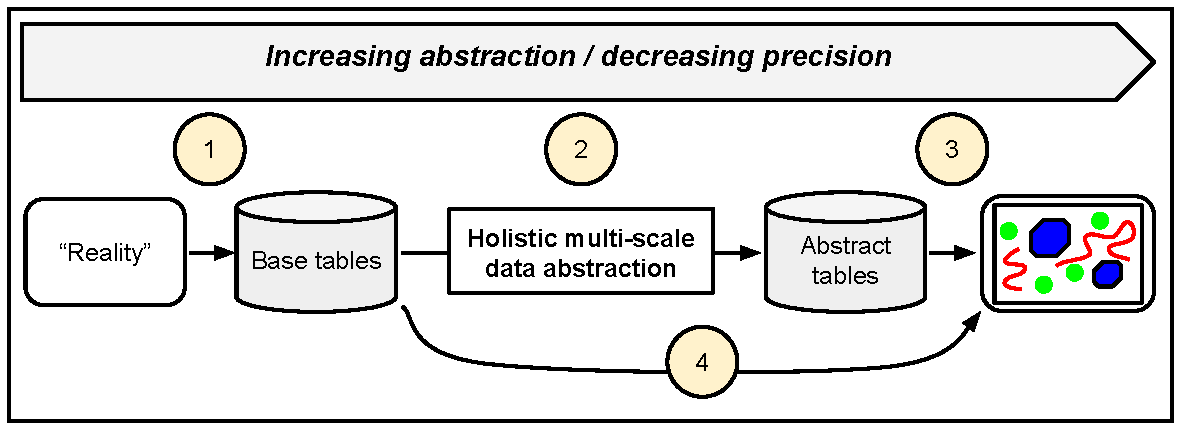
\includegraphics[scale=.6]{figs-thesis/holistic-abstraction-pipeline.pdf}
\caption{A multi-scale data visualization can abstract ``reality'' into visual representation using different paths. The path $\lbrack1,4 \rbrack$ defers all data abstraction to the visual renderer, while the path $\lbrack 1,2,3 \rbrack$ computes a multi-scale data abstraction, which is then accessed by the visual renderer. This figure is modified after Grunreich~\cite{gruenreich1985cag}}
\label{fig:related:work:data:abstraction}
\end{center}
%\vspace*{-4ex}
\end{figure}

To realize further the potential of data visualization, this thesis proposes to bring data abstraction techniques to where the data is frequently managed, i.e. relational database systems (RDBMS). The extension of RDBMS with support for data visualization induces a new class of systems, i.e. data visualization management systems (DVMS)~\cite{wu2014case}. This thesis focuses on four problems that hinder the realization of DVMS.

\subsection{Holistic Multi-scale Selection}
Panning and zooming are powerful techniques that allows users to explore data at different focal points and levels of detail~\cite{stolte2003multiscale,woodruff2001datasplash}. However, computer screens have a finite number of visual configurations by which the data can be represented. To avoid conflicts at lower scales, the set of rows must be abstracted according to principles that ensure legibility~\cite{woodruff1998constant, topfer1966principles}.  for example by selected, aggregated and projected to increase legibility and . Failing that, symbols that visually represent the rows will become increasingly cluttered at lower scales, making it impossible for users to comprehend or interact with the data. Dispite this problem, RDBMS today do not natively support operators that can (easily) express the data abstractions needed for complex, multi-scale data visualizations~\cite{wu2014case}. A critical issue is that rows must be abstracted \emph{holistically}

For example, the selection operator only allows rows to be filtered according to a row-by-row predicate. Critically, records in a data visualization must be selected, i.e. according to global criteria such as legibility and relative importance~\cite{weibel:controls:of:generalization}. Moreover, data must sometimes be consistently selected for several levels of detail, which allows users to explore more data points by zooming in. Some important questions that must be answered are:

\begin{itemize}
\item What use cases must holistic selection cover? 
\item What are the sematics of holistic selection?
\item How should holistic selection be parameterized?
\end{itemize}


%\marcos{Not obvious that SQL is or is not the obvious? So build up the argument: Why declarative versus something else? Argue for declarative (leave minute detail to a system, not to the user. Constructive approach is too time consuming). SQL already exists in databases. Argue that ideal to extend SQL.}

\todo{Reuse arguments from related work section in The Case for Visualization Management Systems~\cite{wu2014case}: % http://www.vldb.org/pvldb/vol7/p903-wu.pdf
\begin{itemize}
\item Previous work in visualization systems have traded-off between expressiveness and performance.
\item D3, protovis, and matplotlib are highly expressive, however they require low-level programming that impedes the ability to quickly iterate and do not scale to large datasets.
\item Declarative grammar-based languages, such as the Grammar of Graphics, and ggplot2 are expressive domain-specific languages designed for rapid iteration, however they do not scale beyond their host environments of SPSS and R.
\item Recent systems address these scalability limitations int two ways
\item First, by either adopting specific data management techniques such as pre-computation (Real-time visual querying of big data),  indexing (Nanocubes for real-time exploration of spatiotemporal datasets), sampling (Blinkdb: queries with bounded errors and bounded response times on very large data), speculation (Distributed and Interactive Cube Exploration), and aggregation (Dynamic reduction of query result sets for interactive visualization, Bin-summarise-smooth: a framework for visualising large data).
\item Second, by developing two-tiered architectures where the visualization client composes and sends queries to a data management backend (Polaris: A system for query, analysis and visualization of multi-dimensional relational databases, Visreduce: Fast and responsive incremental information visualization of large datasets.)
\item The former approaches are optimized towards properties of specific applications or visualization types and may not be broadly applicable.
\item The former approaches are optimized towards properties of specific applications or visualization types and may not be broadly applicable.
\end{itemize}
Managing Data for Visual Analytics: Opportunities and Challenges~\cite{fekete2012dmvis}: % https://hal.archives-ouvertes.fr/file/index/docid/272779/filename/VAChapter_final.pdf
\begin{itemize}
\item Foo
\end{itemize}
}

\subsection{Declarative Specification} 
Designers of visualizations must be able to control the selection of data. While, data abstraction can be expressed in all programming languages, it is generally not easy or time-efficient to specify a holistic selection using imperative commands. A declarative approach, which leaves the minute details to the system, and lets the user focus on higher-level goals, is arguably better. The same type of argument has been made for SQL, which is one of the most successful programming languages for selecting relational data. However, SQL and its corresponding query engines do not support holistic selection. So, for data visualization purposes, SQL must be extended with new syntax for expressing holistic selection. An important questions is:

\begin{itemize}
\item How can SQL be extended to allow designers to express holistic selection?
\end{itemize}

\todo{Reuse arguments from: The Case for Visualization Management Systems~\cite{wu2014case}: % http://www.vldb.org/pvldb/vol7/p903-wu.pdf
\begin{itemize}
\item Foo
\end{itemize}
Managing Data for Visual Analytics: Opportunities and Challenges~\cite{fekete2012dmvis}: % https://hal.archives-ouvertes.fr/file/index/docid/272779/filename/VAChapter_final.pdf
\begin{itemize}
\item Foo
\end{itemize}
}

\subsection{Scalable Data Processing} 
A query executing engine for holistic selection queries must be scalable, because the data may be large. One approach is to translate holistic selection queries to low-level code (e.g. LLVM, C++, OpenMP, or MPI), which can potentially result in very efficient execution. However, low-level code is harder to optimize across platforms. A better approach is to target a higher-level language such as SQL, which reuses optimization techniques that are built-in to SQL query engines~\cite{boncz2005pathfinder, boncz2006monetdb, grust2009ferry}. Additionally, data that underlies a visualization is frequently stored and managed in RDBMS to begin with~\cite{wu2014case}. Therefore, it makes sense to compute holistic selection on top of or inside an RDBMS, e.g. using a translation to pure SQL. Assuming that holistic selection is implemented on top of an RDBMS, some key questions are: 

\begin{itemize}
\item How can holistic selection queries be translated into scalable and efficient queries in pure SQL? 
\item How can the built-in optimizations of relational database engines be leveraged?
\end{itemize}

\subsection{Predictive Data Materialization}

\note{Mention something about the cost of CDN}

Digital maps are a type of visualization of geographical maps. Raw spatial data is transformed into a visual abstraction, the actual map. The transformation data objects to images is relatively CPU and I/O intensive. In a scalable service, we want to materialize and cache the visual abstraction ahead of time as much as possible. In order not to waste CPU and I/O resources, we want to prioritize the materialization of the map by the propabilty that parts of the map are accessed. Most web services today experience highs and lows in the number of concurrent users. If we can predict the content that will be requested during a high load window, we can exploit low-load windows perform pre-materialization. The questions that arise are:
\begin{itemize}
\item How can the prediction process be guided, e.g. by logging data?
\item How can we design a prediction model that works well for geospatial workloads?
\end{itemize}

\section{Contributions of this Thesis}
\label{sec:introduction:contributions}

Instead of presenting a complete system for creating and serving data visualizations, this thesis concentrates on specific aspects of building such a system. In Chapter~\ref{chapter:case:study} we will show how the contributions can be integrated with existing systems: a relational database (PostgreSQL with PostGIS extension) and commercial key-value stores (Redis and WMTS).

The contributions of this thesis cover two topics: global selection for data-driven visualizations (see Sections~\ref{sec:introduction:contributions:cvl}~and~\ref{sec:introduction:contributions:glossy}), and adaptive pre-emptive caching of geographical data (see Section~\ref{sec:introduction:contributions:tileheat}).

%Short something about how the problems stated in Section~\ref{sec:introduction:problem:statement} are addressed.
 
\subsection{Global Selection for Geographical Maps with Zoom Consistency}
\label{sec:introduction:contributions:cvl}

Something resembling the abstract

\subsection{Global Selection for Data Visualizations}
\label{sec:introduction:contributions:glossy}

Something resembling the abstract. 

\subsection{Prediction of Geospatial Key-Value Workloads}
\label{sec:introduction:contributions:tileheat}

Something resembling the abstract

\subsection{Publications}

Some of the chapters in this thesis have been previously published in or submitted to international conferences. The publications and submissions are listed below: 

\begin{itemize}
\item \textbf{Chapter~\ref{chapter:cvl} -- Declarative Cartography~\cite{declarative:cartography}}: Pimin Konstantin Kefaloukos, Marcos Vaz Salles, and Martin Zachariasen. Declarative Cartography: In-Database Map Generalization of Geospatial Datasets. In ICDE, 2014. 
\item \textbf{Chapter~\ref{chapter:glossy} -- Glossy~\cite{glossy}}: Pimin Konstantin Kefaloukos, and Marcos Vaz Salles. Glossy: Global Selection for Data Visualizations. In submission. 
\item \textbf{Chapter~\ref{chapter:tileheat} -- Tileheat~\cite{tileheat}}: Pimin Konstantin Kefaloukos, Marcos Vaz Salles, and Martin Zachariasen. Declarative Cartography: In-Database Map Generalization of Geospatial Datasets. In SIGSPATIAL, 2012. 
\end{itemize}

\subsection{Data and Software}

Mention where Git repos are and what they contain.

\section{Structure}
\label{sec:introduction:structure}

The remainder of this thesis is organized as follows. Chapter~\ref{chapter:state:of:the:art} covers the state of the art data abstraction and scalable key-value stores. Chapter~\ref{chapter:case:study} presents a case study of the Danish Geodata Agency, which as part of the public sector in Denmark publishes high-quality currated geospatial data, e.g. for visualization purposes. This chapter also contains a light-weight manual for anyone wishing to implement the contributions of this thesis. Chapters~\ref{chapter:cvl}, ~\ref{chapter:glossy}, and ~\ref{chapter:tileheat} cover the theoretical and experimental details of the main contributions this thesis. Chapter~\ref{chapter:conclusion} presents the conclusions of this thesis and discusses directions for future work.


%  ############
%  #  CHAPTER  
%  ############ 

\chapter{Related Work}
\label{chapter:related:work}

\marcos{Related work chapter: here are the broad areas (paint the big picture). Maybe even a real picture, a figure that shows the different areas. A conceptual model of how to navigate the litterature, a map of sorts. Here are some representative works, here is how you should think about them. There will be some references, details in the related works. focus on data abstraction (map generalization, also cover some other stuff), less focus on data serving (database, key-value stores, caching, CDN, etc.).}

\pitfall{\emph{I Am So Unique:} Do not ignore previous work when writing up your paper. You have to convince the reader that you have done something new, and the only way to do that is to explain how it is different than what has already been done. All research takes place in some kind of intellectual context, and your job as author is to situate what you have done within a framework of that context. A good previous work section is a mini-taxonomy of its own, where you decide on meaningful categorization given your specific topic. Proposing new names for old techniques or ideas may sneak your work past some reviewers, but will infuriate those who know of that previous work. This tactic will also make you lose credibility with knowledgeable readers. If you cannot find anything related to what you have done, it?s more likely that you?re looking in the wrong subfield than that your work is a breakthrough of such magnitude that there is no context. Remember to discuss not only work that has been done on similar problems to your own, but also work that uses similar solutions to yours that occurs in different problem domains. This advice is even more critical if you were lax about doing a literature review before you started your project. If you find work similar to your own, you have a fighting chance of carefully differentiating yours in the writeup, but if a reviewer is the one to
bring it to your attention, the paper is most likely dead.}

\pitfall{\emph{Enumeration Without Justification:} Simply citing the previous work is necessary but not sufficient. A description that 'X did Y', even if it includes detail, is not enough. You must explain why this previous work does not itself solve your problem, and what specific limitations of that previous work your approach does address. Every paper you cite in the previous work section is a fundamental challenge to the very existence of your project. Your job is to convince a skeptical reader that the world needs your new thing because it is somehow better than a particular old thing. Moreover, it's not even enough to just make the case that yours is different: yours must be better. The claims you make must, of course, be backed up by your validation in a subsequent results section.

A good way to approach the previous work section is that you want to tell to a story to the reader. Figure out the messages you want to get across to the reader, in what order, and then use the references to help you tell this story. It is possible to group the previous work into categories, and to usefully discuss the limitations of the entire category.}

To address the short-comings of GIS for the web, this dissertation makes the case for a new system category, Map Visualization Management Systems (MVMS). An MVMS should address three crucial questions:

\begin{enumerate}
\item How can non-experts intuitively express the creation of multi-scale map visualizations?
\item How can map systems scalably process millions of geographical records?
\item How can map systems scalably serve map visualizations to millions of online users, who expect 24~x~7~availability and acceptable latency?
\end{enumerate}

Answering each of these questions will require us to investigate areas beyond pure map visualization. For example, work in \emph{map generalization} addresses the problem of geographical data abstraction for multiple scales~\cite{weibel1999generalising}; work in \emph{data management} addresses the issue of managing data for visualizations; work in \emph{programming languages} addresses the issue of expressing the data transformations~\cite{sql}; work in \emph{graphics} addresses the issue of representating data visually~\cite{wickham2009ggplot2, wilkinson2006grammar}; work in \emph{data management} addresses the issue of processing millions of records~\cite{wow-so-many-to-choose-from}; work in \emph{distributed systems} addresses the issue of serving data to millions of users~\cite{wow-so-many-to-choose-from}. All of these topics play a key role in map visualization. This chapter scans the intersection between map visualization and the related work and compares the results against the requirements of a Map Visualization Management System (see Chapter~\ref{cha:introduction}).


% FORMAT:
% section{FIELD}
% RELEVANCE TO MAP VISUALIZATION
% subsection{CONTRIBUTION} plus-minus
% subsection{CONTRIBUTION} plus-minus

\section{Geographical Information Systems}

Constraint-based map generalization (Cartography and Geographic Information Science)~\cite{harrie1999constraint}.


\section{Databases}

Reverse Data Management (VLDB)~\cite{meliou2011reverse}

Scalar (IEEE Big Data)~\cite{battle2013scalar}.

Google Fusion Tables (SIGMOD)~\cite{gonzalez2010fusiontables}, scalable data processing, scalable data serving, intuitive visual abstraction interface, however non-configurable data abstraction interface.

CartoDB~\cite{cartodb2014cartodb}.

HadoopGIS (VLDB)~\cite{aji2013hadoopgis}.

Ermac (VLDB)~\cite{wu2014case}

Analytic Data Engine for Visualization in Tableau (SIGMOD)~\cite{wesley2011tableau}.

Distributed Declarative Constraint Optimization (VLDB)~\cite{liu2012cologne}

Efficient Spatial Sampling (SIGMOD)~\cite{sarma2012fusiontables}.

Select-Distinct queries~\cite{nutanong2012multiresolution}.

\section{Programming Languages}

As they relate to data transformation for data visualization.

\subsection{Graphics Languages}

Examples: The Grammar of Graphics, ggplot2

Why not good enough? Not holistic

\subsection{Declarative Languages}

Examples: SQL, datalog

Why are they not good enough? Hard to write holistic programs.

\subsection{Linear Programming}

Give examples: Das Sarma, Landcover.

Why is it not good enough? Hard to write, and require us to know the data, making programs hard to reuse. Plus side is that they capture constraints and objectives.


\section{Databases}

As they relate to data processing for data visualization. Specifically, in-database processing of data transformation. 

Examples: xQuery, Ferry, Scalar, Ermac

Why not good enough? Good idea, but lack compilations for holistic programs

\subsection{Conclusion}

Reverse Data Management is the right abstraction.

\section{Distributed Systems}

As they relate to data serving for data visualization.

\subsection{Data Partitioning}

Key-value stores, tile pyramids, vector tiles, buckets, 

\subsection{Data Replication}

content delivery networks

\subsection{Content Delivery Networks}


\section{Holistic Data Abstraction}

Obviously, this is a core field

\subsection{Map Generalization}

Operators

Constraints

Selection

Displacement

Aggregegation





\section{Visual Conflicts}

Constraint-based visualization~\cite{harrie1999constraint}. Constant Information Density~\cite{woodruff1998constant} and Toepfer~\cite{topfer1966principles}. Binary object relations, e.g. 9-intersection~\cite{egenhofer1991categorizing} and RCC~\cite{randell1992spatial}. Object set mapping~\cite{sarma2012fusiontables, kefaloukos2014cvl}.

Bertin~\cite{jacques1967semiologie}, Nickerson~\cite{nickerson1994visual}, Tufte~\cite{tufte1983visual}.

Detecting conflicts by indexing~\cite{nutanong2012multiresolution, kefaloukos2014cvl}, 

Star and ladder~\cite{foerster2010challenges}, zoom consistency~\cite{sarma2012fusiontables}. Multi-scale Select-Distinct~\cite{nutanong2012multiresolution}.



% http://youtu.be/nLjVKOLyvx4
% Since maps are constructed in finite spaces, real-estate is at a premium. As such, not everything is represented, and even those things that are represented are not necessarily represented precisely. You can see a couple of examples here. Roads, rivers, cities, towns and islands are the most common victims of something like this. - Matt Dube, see http://www.spatial.maine.edu/~matthew.dube/


%  ############
%  #  CHAPTER  
%  ############ 

\chapter{Case study: The Digital Map Supply}
\label{chapter:case:study}

\section{Why Public Geographical Data is Important}

\begin{enumerate}
\item Take Anders' write-up (if I can find it). Either attribute or paraphrase it . Probably paraphrase and do not forget to thank him in acknowledgements.
\item Cite offentlige data is spil, etc.
\end{enumerate}

\section{The Digital Map Supply Today}

%\begin{itemize}
%\item Diagram of Users and Providers
%\end{itemize}

\subsection{Requirements}
\begin{itemize}
\item SLA
\end{itemize}

\subsection{Architecture and metrics}
\begin{enumerate}
\item Describe the key metrics
\item Describe the architecture (tiers, number of data centers, services running)
\end{enumerate}

1:  Budget, Requests per day, Peak Load, Unique accounts, Spatial skew, Temporal skew, Performance sensitivity, Availability over time (find Kenneths tal)

\begin{figure}[tb]
  \begin{center}
    \begin{tabular}{cc}
      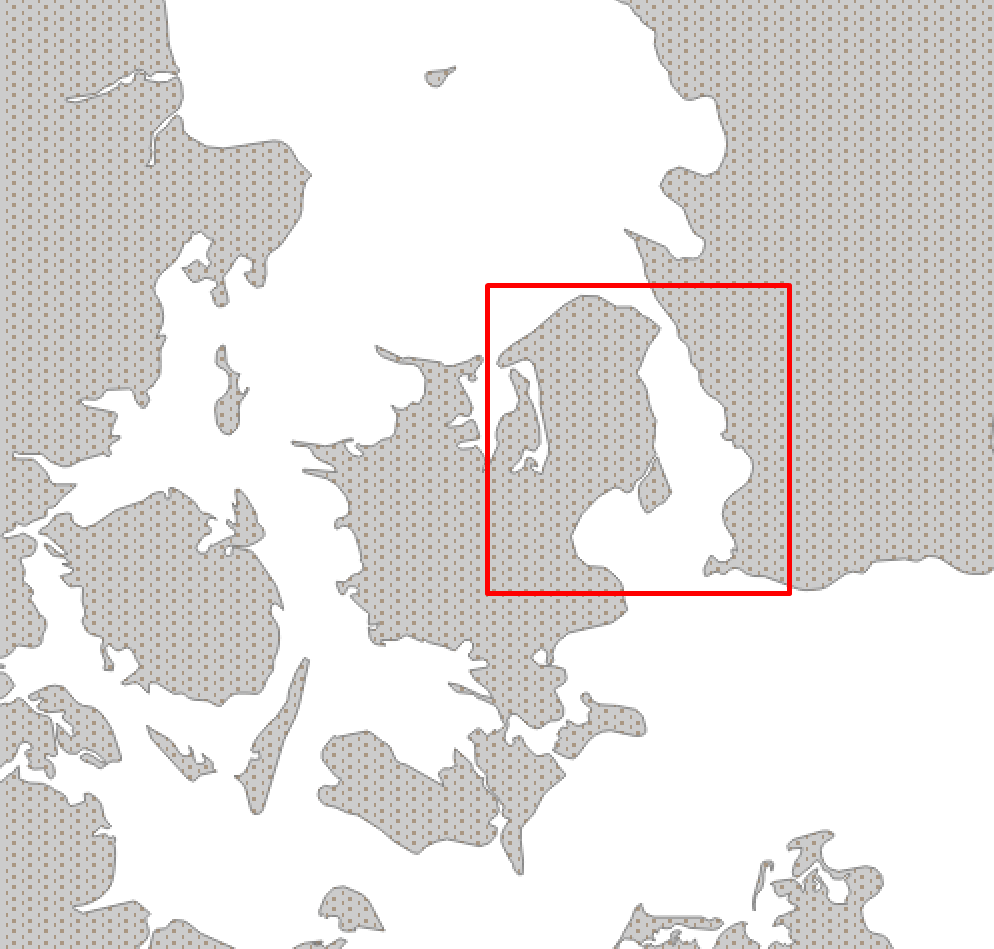
\includegraphics[width=0.4\linewidth]{./figs-thesis/heat_extent.png} & 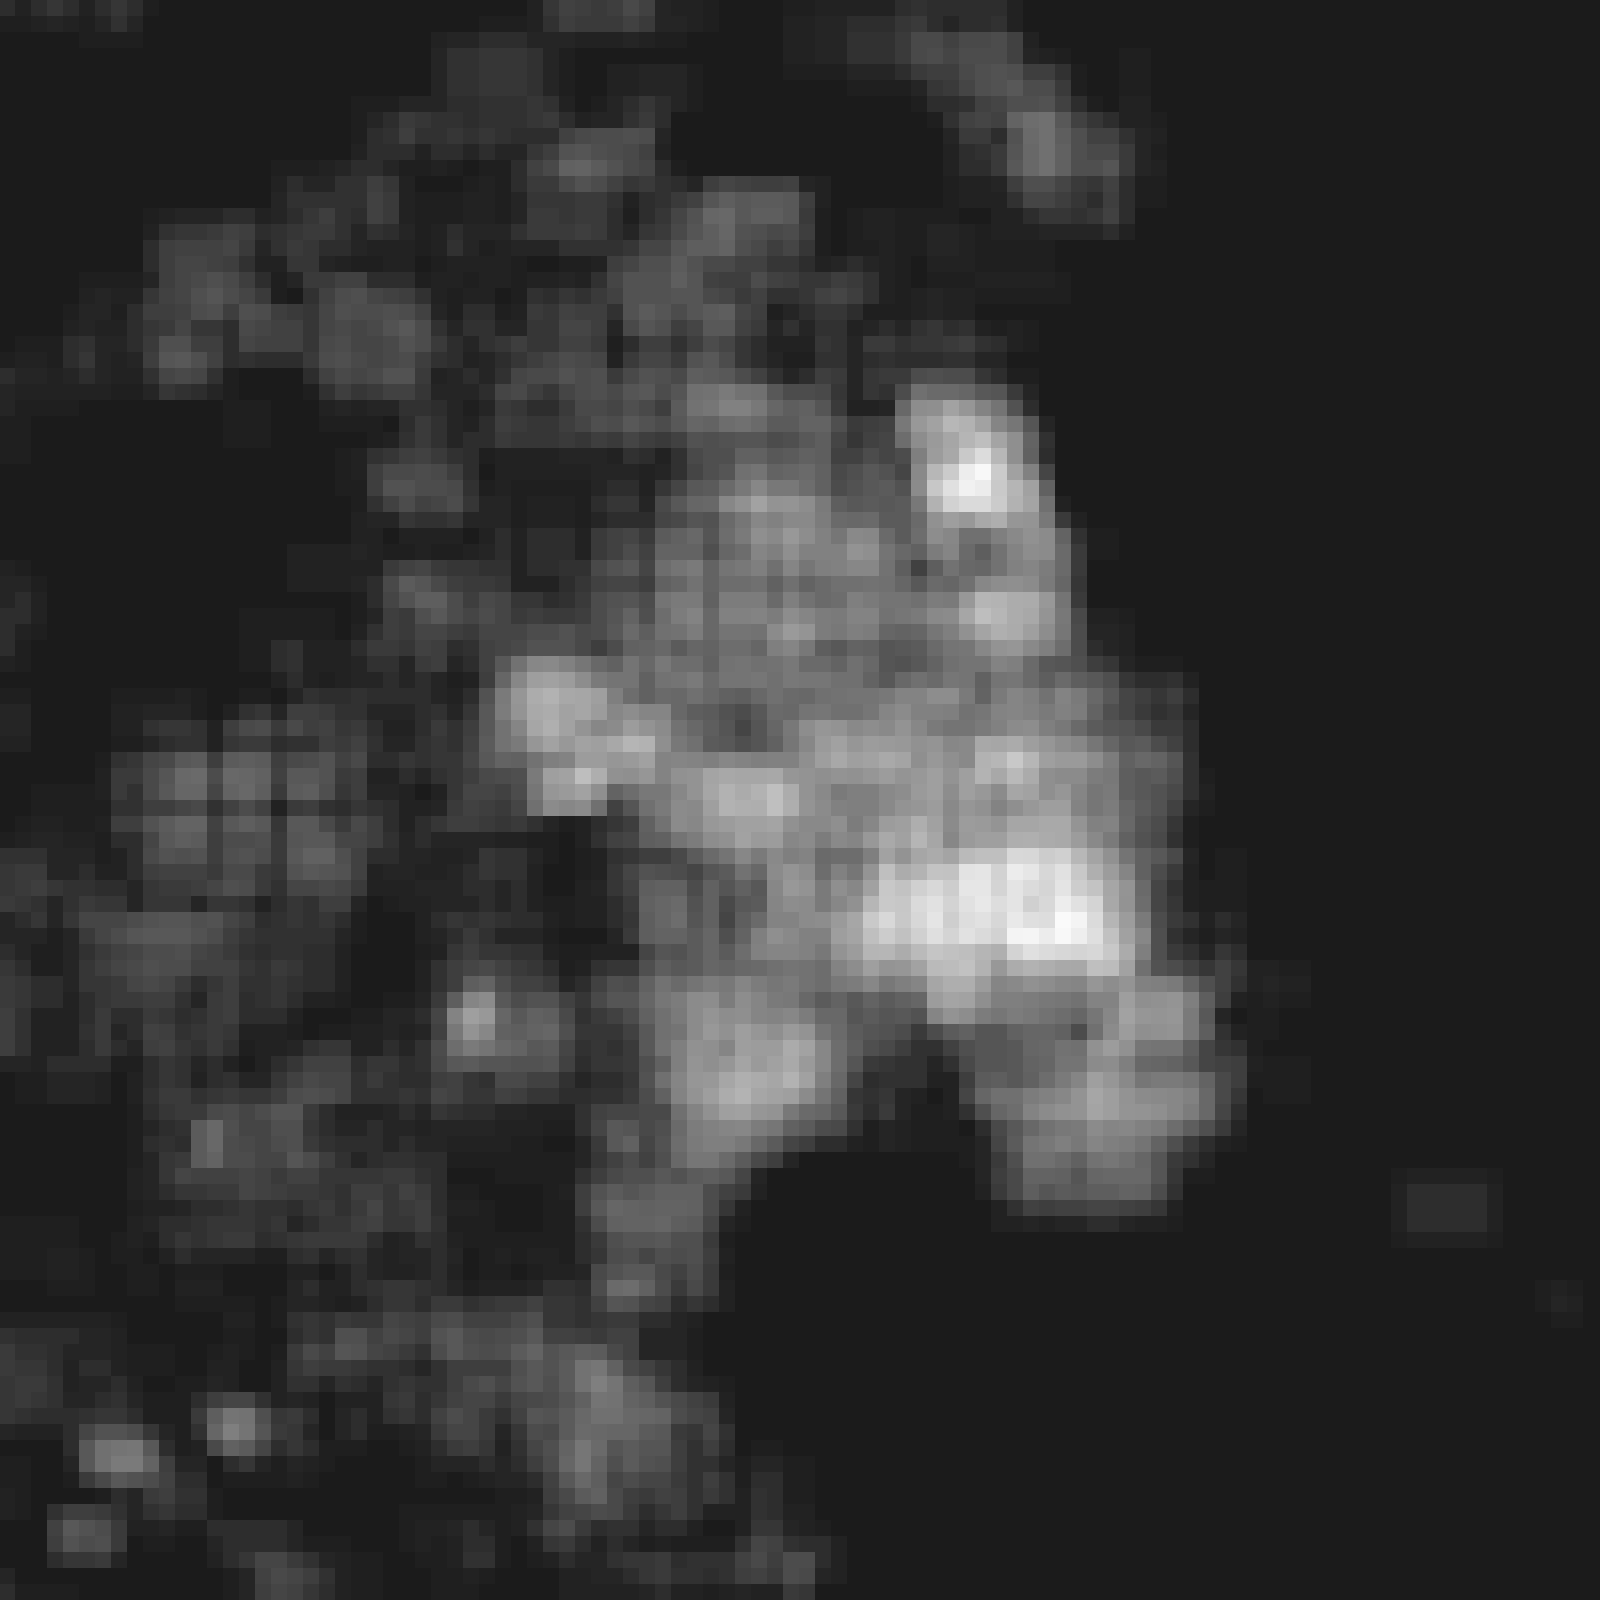
\includegraphics[width=0.383\linewidth]{./figs-thesis/tileheat_heatmap_sjaelland.png} \\
    \end{tabular}
    \caption{Foo.}
    \label{case:study:heat:map}
  \end{center}
\end{figure}

\subsection{Challenges and Opportunities}
\begin{itemize}
\item Availability, especially for multi-source applications
\item Performance sensitivity
\end{itemize}	
% 99% is not high availability 
% 200 ms is not low latency
% Images are not an interactive experience


\begin{figure}[htbp]
\begin{center}
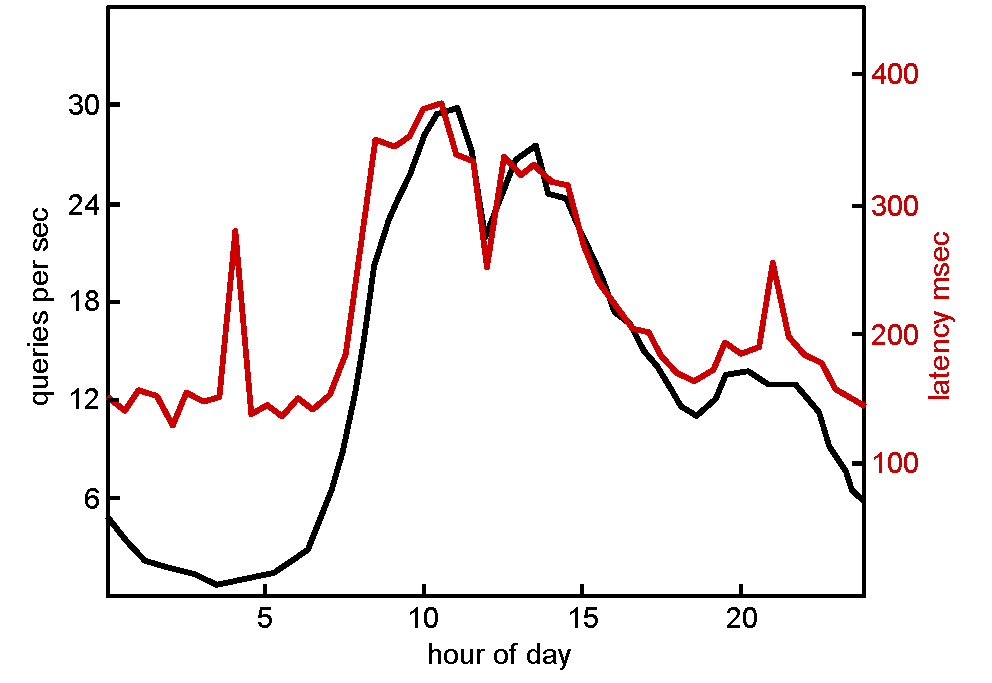
\includegraphics[scale=.8]{figs-thesis/load-latency-correlation.pdf}
\caption{\emph{Temporal query skew:} Default}
\label{default}
\end{center}
%\vspace*{-4ex}
\end{figure}

\begin{figure}[htbp]
\begin{center}
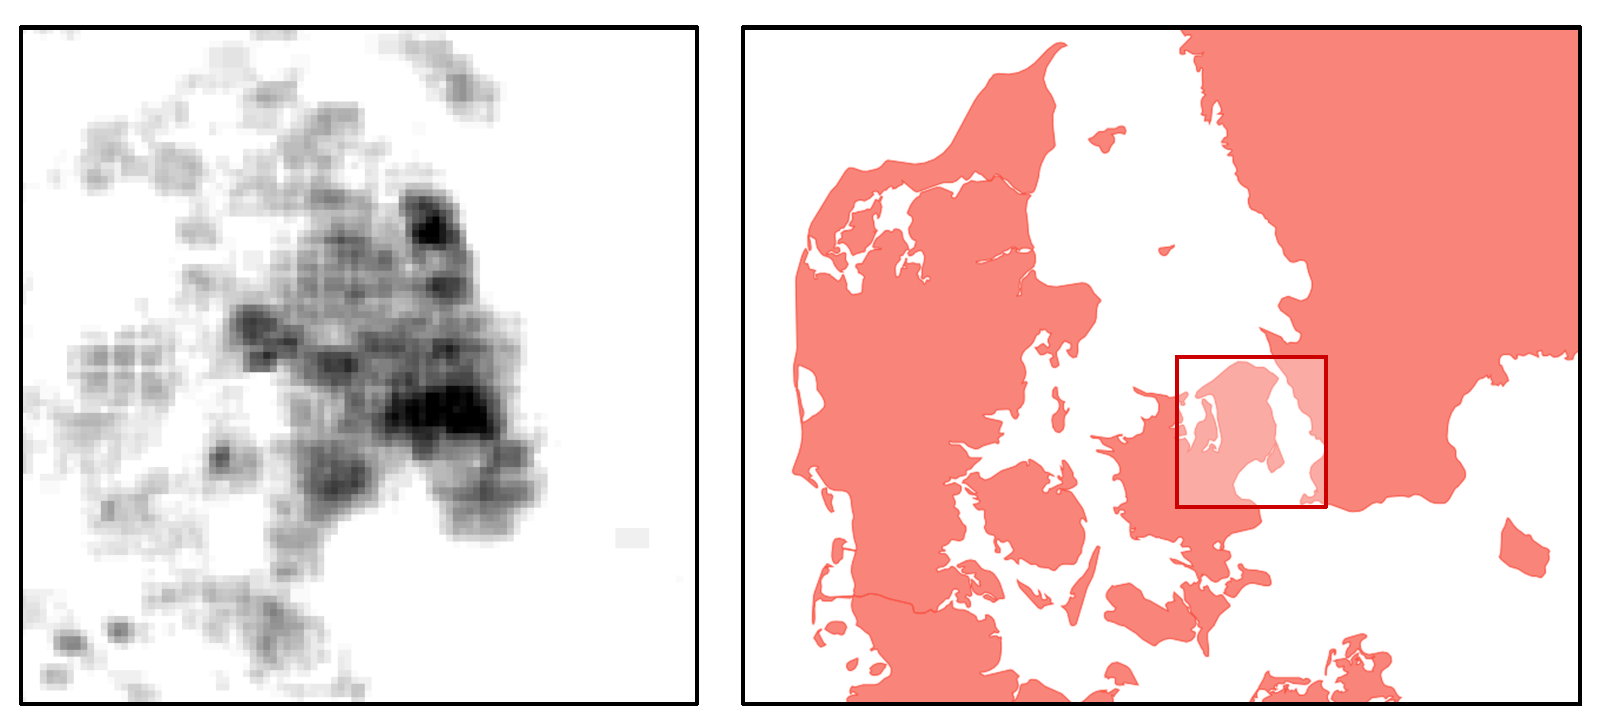
\includegraphics[scale=.5]{figs-thesis/heatmap-side-by-side.pdf}
\caption{\emph{Spatial query skew:} Default}
\label{default}
\end{center}
%\vspace*{-4ex}
\end{figure}

\section{Using the Contributions of this Thesis}

\subsection{Glossy}

\subsection{Tileheat}

\section{Summary}


\chapter{Declarative Cartography: In-Database Map Generalization of Geospatial Datasets}
\label{chapter:cvl}
\lstset{
  language=cvl
}

\section{Introduction}
\label{sec:cvl:introduction}
The goal of map generalization is to produce a map at a given scale that achieves the right balance between rendering performance and information quality for end users. For example, in a tourist attraction rating system, one needs to efficiently visualize important attractions, and constrain object proximity to allow space for user interaction. In a journalistic piece that maps traffic incidents, however, maintaining the underlying distribution of data is the most important aspect, but at the same time object density must be constrained to ensure high-performance data transfer and rendering.

Fully automatic generalization of digital maps~\cite{sarma2012fusiontables,nutanong2012multiresolution} is relevant in many areas such as social networks, factivism and data journalism~\cite{cohen2011journalism,bono,sankaranarayanan2009twitterstand}, where there is a constant need for visualizing new and often massive geospatial datasets. Automatic generalization includes both data reduction and graphical rendering~\cite{weibel1999generalising,gruenreich1985cag}. Increasingly, graphical rendering is deferred to map clients. This trend leaves the challenging problem of data reduction, i.e., selecting the right information to be displayed across zoom levels of the map, to the map service provider~\cite{gaffuri12vectortiles}. 

Both the performance and quality of a generalized map become important as the map gains a large audience. A map generalization solution handling data reduction in this context should be able to deal with big spatial datasets, consisting of both point and polygon records, should be usable by novice programmers, and should be able to finish processing quickly, e.g., in time for a tight news agency deadline. Ideally, such a system will allow users to control the important aspects of generalization solutions using logical and concise measures and reuse existing technology as much as possible, e.g., relational database technology.

Unfortunately, current approaches for data reduction in map generalization fall short in one or many of the above dimensions. Recent work has mostly considered only explicit rules or pre-set constraints for map generalization, resulting in solutions that are either too tedious~\cite{sld,mapnik}, or too restrictive for users~\cite{sarma2012fusiontables,nutanong2012multiresolution}. In addition, previous solutions have been poorly integrated with existing technology, resulting in scalability bottlenecks such as being restricted to the main memory capacity of a single node~\cite{sarma2012fusiontables}. 
 

Spatial data is often stored in a database with powerful spatial extensions installed, so a natural idea is to exploit the processing capabilities of the database to perform map generalization. In this work, we present a novel \emph{database-integrated} approach that is a complete solution to the data reduction problem in map generalization. All operations are performed entirely within the database process, and the result is a preprocessing of spatial records for fast execution of subsequent scale-parameterized queries~\cite{hilbert1891ueber}. Essentially, a number is assigned to each spatial record corresponding to the lowest zoom-level at which the record should be visible in a zoomable map, allowing for efficient indexing.

Using a \emph{declarative language}, we allow the user to concisely express spatial constraints and object importance, which are used to compute a multi-scale database from an input table of spatial data. This gives users a large amount of control over the map generalization process, while still being extremely concise, expressing a generalization with as little as four lines of code. 

We term our approach \emph{declarative cartography}\, since it combines a declarative language for data reduction with a compilation procedure that results in efficient database programs to transform data for cartographic visualization.

In this paper, we make the following four contributions:
\begin{enumerate}
\item We present a declarative language, Cartographic Visualization Language (CVL, pronounced ``civil''), for generalizing spatial datasets. CVL is designed to be simple and concise to use for novice programmers. The CVL language was designed in collaboration with the Danish Geodata Agency and Grontmij in Denmark.\footnote{\url{http://www.gst.dk/English/}}\footnote{\url{http://grontmij.dk/}}

\item We convert the data reduction problem in map generalization to an instance of the well-known \emph{set multicover problem}~\cite{rajagopalan1998primal}, which makes constraints fully pluggable and allows reuse of well-known algorithms~\cite{rajagopalan1998primal,vazirani2001approximation}.

\item We show how to fully evaluate CVL inside the database; this enables us to reuse basic database technology for data management and scalability. While CVL is designed to compile to a variety of engines~\cite{Stonebraker:2010:PDBMSvsMapReduce}, we present here an implementation using a relational database engine with spatial extensions. The code for the project is available as open source through the project website.\footnote{\url{http://github.com/dmslab/declarativecartography}}

\item We present experimental results for a variety of real datasets. The results show that the proposed approach has good performance and produces high-quality map generalizations.
\end{enumerate}

In Section~\ref{sec:cvl:background}, we define the data reduction problem in map generalization as a selection problem. In Section~\ref{sec:cvl:language}, we introduce the CVL language. In Section~\ref{sec:optimizationmodel}, we formalize the selection problem as a combinatorial optimization problem based on a mapping to the set multicover problem, and we revisit algorithms for this problem in Section~\ref{sec:cvl:algorithms}. In Section~\ref{sec:implementation}, we discuss the compilation procedure that enables us to run CVL on a relational database backend. Experimental results are presented in Section~\ref{sec:experimental}, and finally related work is summarized in Section~\ref{sec:cvl:related:work}.

\section{Selection of Geospatial Data}
\label{sec:cvl:background}

In the \emph{selection problem,} we wish to select the subset of a geospatial dataset to be visualized on a map at a given scale. Below we define the basic components of the problem, and informally define the associated optimization problem.

\subsection{Geospatial records and weights}
\label{sec:cvl:records}

The dataset is assumed to consist of a set of \emph{geospatial records} drawn from a database table. The schema of a geospatial record consists of a \emph{geometry} field (e.g. a point, line or polygon), a \emph{unique ID} field and any number of additional textual and numeric fields, such as ``city name'' and ``population''.

Each record is assigned a \emph{user defined weight} using CVL (see Section~\ref{sec:cvl:language}). The weight models the importance of a record, with high weight corresponding to great importance. Any subset of records --- or all records for that matter --- may have the same weight. Therefore, the weights induce a partial order of the records.

\subsection{Zoom levels and map constraints}
\label{sec:cvl:constraints}
For zoomable maps, different subsets of the data should be selected for display at different scales or \emph{zoom levels}. Let the zoom-levels run from 1 (lowest scale) to $\mathcal{Z}$ (largest scale). On a given zoom level, the map is rendered at a certain pixel resolution. Thus, for a given zoom level, we know the distance in pixels between geospatial locations. This gives rise to two particularly important map constraints~\cite{harrie2007modelling} when selecting data for a given zoom level.

Firstly, the \emph{principle of constant information density} implies that the number of records that can be displayed within an area of a certain pixel size should be bounded~\cite{topfer1966principles}. Assume that we divide the complete map into cells (or tiles) of, say, 256 x 256 pixels. The \emph{visibility} constraint states that each cell can contain at most $K$ selected records, where $K$ is a user-defined parameter~\cite{sarma2012fusiontables}.

Secondly, records cannot be too close to each other in the map --- otherwise the user will not be able to clearly distinguish between them. The \emph{proximity} constraint states that every pair of visible records must be separated by at least $d$ pixels, where $d$ is a user defined parameter.

In addition to these constraints that must hold separately for each zoom level, there are constraints that must hold across zoom levels. A particularly important constraint is the \emph{zoom-consistency} constraint, which states that when a record is filtered out at a given scale, it should also be filtered out at all \emph{lower} scales~\cite{sarma2012fusiontables}. When a user zooms out on a map, records can only disappear --- not reappear.

Apart from the zoom-consistency constraint, CVL supports constraints based on \emph{simple measures} that are \emph{satisfiable by selection} (see Section~\ref{sec:cvl:language}). A simple measure is a function that maps a set of records to a scalar value. A constraint is violated if the measure exceeds a threshold. A constraint is satisfiable by selection if we can \emph{always} satisfy it by simply deleting an appropriate subset of the records. Both the visibility and proximity constraints respect these restrictions. However, we cannot model constraints that have complex measures or cannot be satisfied by using selection alone, such as \emph{topology} and \emph{spatial distribution} constraints. We leave these classes of constraints to future work.

\subsection{Conflicts}
\label{sec:cvl:conflicts}

Constraints such as visibility or proximity can be modeled using the notion of \emph{conflicts}. A conflict is a set of records that cannot all be selected without violating the constraint.

For the visibility constraint, there is a conflict generated for every cell that contains more than $K$ records. For the proximity constraint, there is a conflict generated for each pair of records that is less than $d$ pixels apart (see Figure~\ref{fig:cvl:proximity:conflict}). A record can be in several conflicts, which is the case for point $p$ in the example shown in the figure. A solution to the selection problem is \emph{feasible} if there are no conflicts.

\begin{figure}[htbp]
\begin{center}
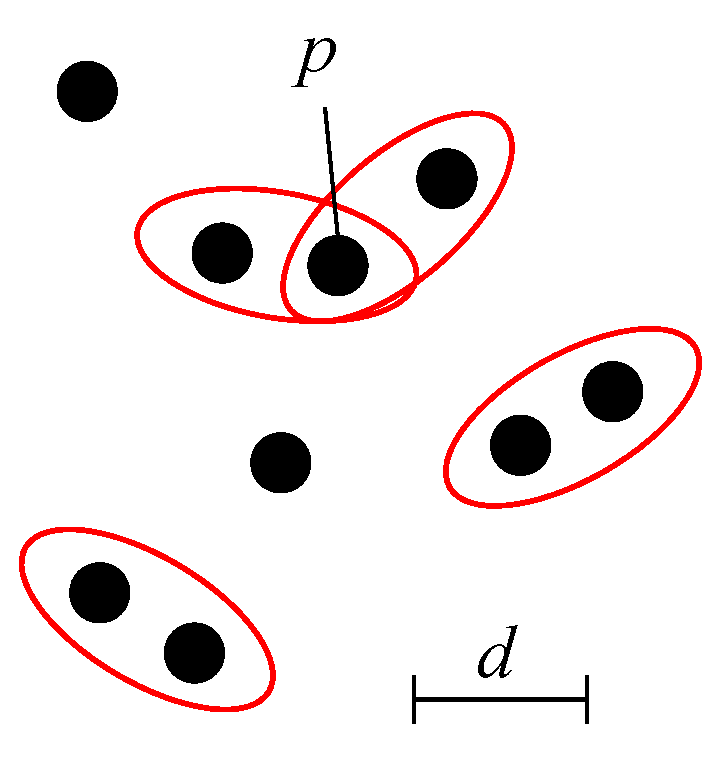
\includegraphics[scale=.3]{figs-cvl/cvl_proximity_conflicts.pdf}
\caption{Conflicts generated by the proximity constraint for distance $d$. Notice that point $p$ is a member of more than one conflict.}
\label{fig:cvl:proximity:conflict}
\end{center}
\vspace*{-4ex}
\end{figure}

Consider a conflict involving $k_1$ records, where at most $k_2$ of these records can be selected (where $k_1 > k_2$). Then it is equivalent to state that at least $\lambda = k_1 - k_2$ of these records must be \emph{deleted}. In the mathematical formulation of the problem in Section~\ref{sec:optimizationmodel}, we will use this alternative way to formulate conflicts.

\subsection{Selection as an optimization problem}
\label{sec:cvl:filtering}
The notion of conflicts is used to define the feasibility of solutions to the selection problem. This should be accompanied by a way to discriminate between solutions. Assigning an importance measure to each record, namely the record weights, intuitively allows us to measure the ``loss of importance'' due to records that are deleted.

In the optimization version of the problem, we seek the feasible solution that minimizes the aggregate weight of records that are deleted. In Section~\ref{sec:optimizationmodel}, we present a mathematical formulation of the selection optimization problem.

For a zoomable map with $\mathcal{Z}$ zoom levels, we are interested in finding $\mathcal{Z}$ solutions to the selection problem, one for each zoom level $i \in \{ 1, \ldots, \mathcal{Z} \}$. We call this problem the \emph{multi-scale selection problem}. To control the way in which we compute these solutions, we use an algorithmic framework known as the \emph{ladder} approach~\cite{foerster2010challenges}. This is a recursive approach, where the output of selection at large scale is used as input to selection at a smaller scale. This means that the zoom-consistency constraint (Section~\ref{sec:cvl:constraints}) is automatically satisfied.

The ladder approach is not appropriate for all use cases. For example, when regional labels are modeled as geospatial records, e.g., the label ``Europe'', we may wish to show a record only on intermediate zoom levels, violating zoom consistency. Handling these use cases would require an alternative formulation, e.g., following the \emph{star} approach~\cite{foerster2010challenges}. This is an interesting avenue for future work.  


\section{CVL Language}
\label{sec:cvl:language}
The Cartographic Visualization Language (CVL) is a declarative language that can be used to specify an instance of the multi-scale selection problem (Section~\ref{sec:cvl:filtering}). CVL is a rule-based language with a similar goal as other rule-based languages for selection over spatial datasets, i.e., to control the density of information at each zoom-level~\cite{sld,mapnik}. The CVL approach is, however, markedly different. In the related languages, the user must explicitly control the selection of records at each zoom level, while also specifying how records are to be visualized. First of all, CVL focuses only on selection, not presentation. Furthermore, CVL controls selection in a novel constraint-based way. Instead of having the user explicitly control the selection of records at each zoom level, CVL lets the user choose map constraints that are instead enforced at all zoom levels. By making the constraints explicit and the control implicit, a very concise formulation is obtained (see Figure~\ref{fig:cvl:example:airports} for an example).

CVL is one of the first languages and frameworks to implement the vision of reverse data management~\cite{meliou2011reverse}. In reverse data management, the core idea is that a user states a set of constraints and an objective. These are given together with an input database to an optimization algorithm which computes an output database that is feasible and optimal with regard to the constraints and objective (if a feasible solution exists). This is exactly how CVL works. Furthermore, a feasible solution is guaranteed to exist, as deleting all records is always a feasible solution.

The CVL language has two statements, the \emph{generalize} statement (see Section~\ref{sec:cvl:generalize:statement}) and the \emph{create-constraint} statement (see Section~\ref{sec:cvl:create:constraint:statement}). The create constraint statement is used to formulate new map constraints and the generalize statement is used to specify a solution to the multi-scale selection problem subject to those constraints.

The CVL language builds on top of SQL and reuses SQL as a language for formulating constraints and record weighting schemes.

\begin{figure}[!t]
\begin{center}
\begin{lstlisting}
GENERALIZE 
   {input} TO {output}
WITH ID {expression}
WITH GEOMETRY {expression}
AT {integer} ZOOM LEVELS
WEIGH BY
  {float expression}
SUBJECT TO 
   {constraint} {float parameters} [AND
   {constraint} {float parameters} [AND
   ...]]
\end{lstlisting}
\vspace*{-1ex}
\caption{Syntax of generalize statement.}
\label{fig:cvl:generalize:syntax}
\end{center}
\vspace*{-4ex}
\end{figure}

\subsection{Generalize statement}
\label{sec:cvl:generalize:statement}

\begin{figure*}[tb]
  \begin{minipage}{0.329\linewidth}
    \centerline{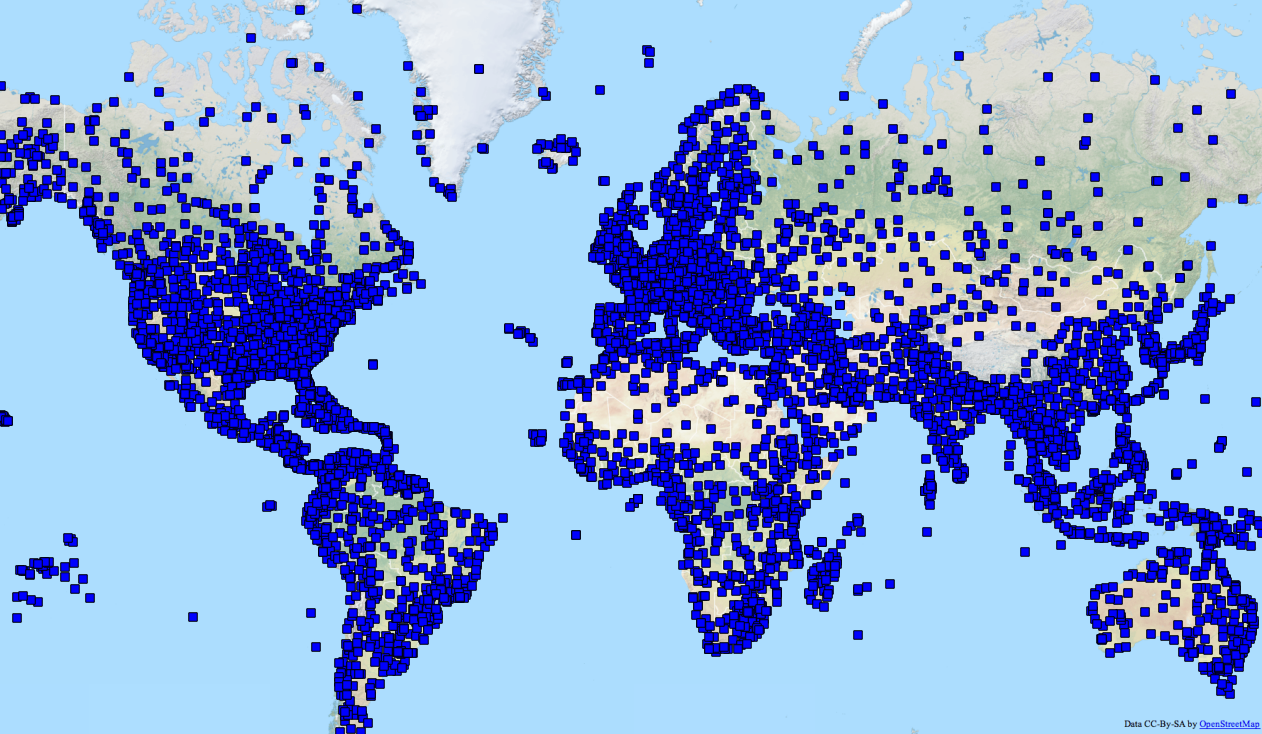
\includegraphics[width=0.95\linewidth]{./figs-cvl/airports.png}}
    \centerline{(a) Full Openflights Airport dataset}
  \end{minipage} \hfill
  \begin{minipage}{0.329\linewidth}
    \centerline{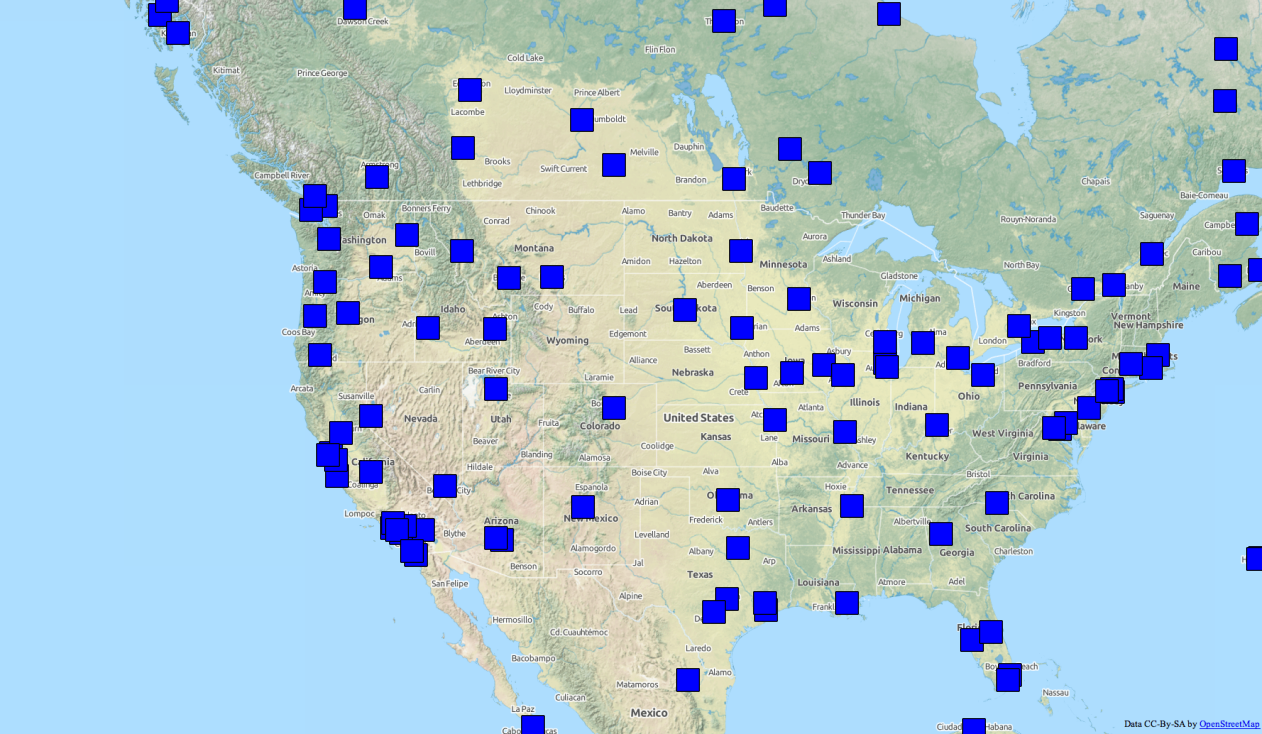
\includegraphics[width=0.95\linewidth]{./figs-cvl/airports_z4.png}}
    \centerline{(b) Airports on zoom-level 5}
  \end{minipage} \hfill
  \begin{minipage}{0.329\linewidth}
    \centerline{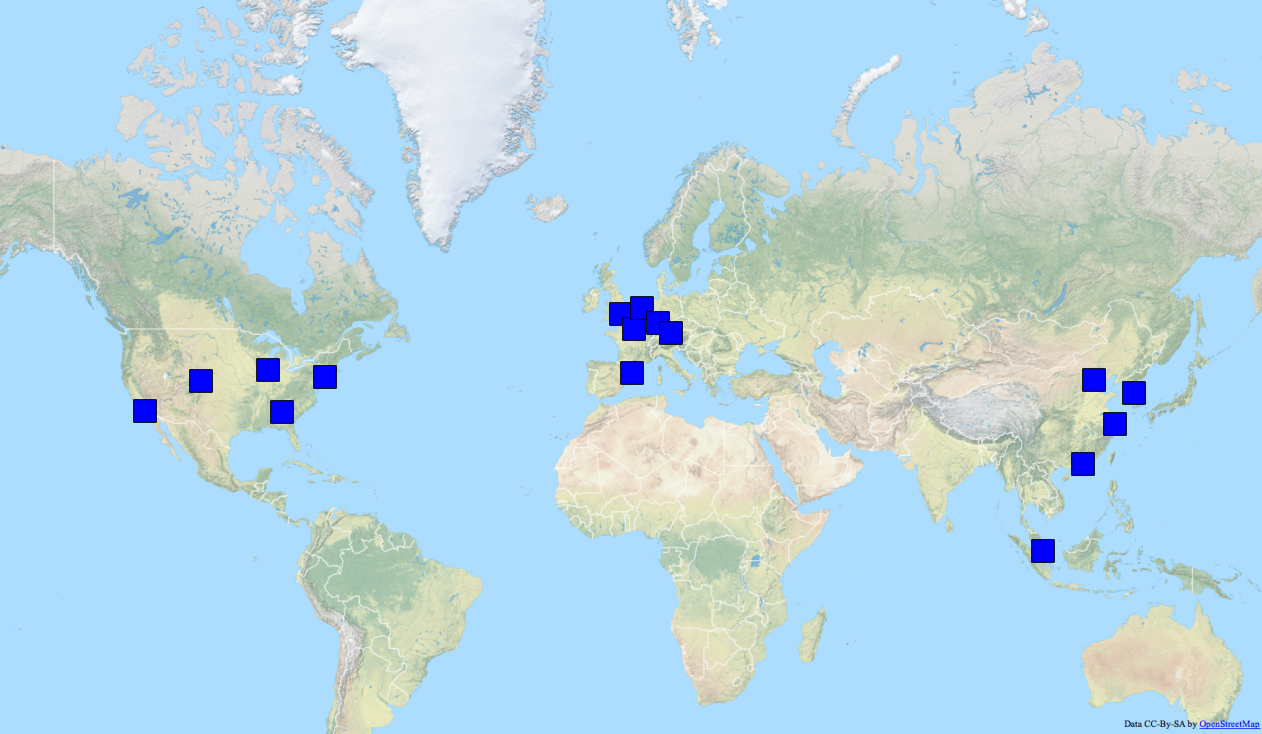
\includegraphics[width=0.95\linewidth]{./figs-cvl/airports_z0.png}}
    \centerline{(c) Airports on the top-most zoom-level.}
  \end{minipage}
  \vspace{-0ex}
  \caption{Airport map (7K points) before (a) and after (b, c) running CVL. The output corresponds to the CVL statement in Figure~\ref{fig:cvl:example:airports}.}
  \label{fig:cvl:visualization:airport}
  \vspace{-2ex}
\end{figure*}

The generalize statement is the main statement in CVL. This statement creates a new multi-scale dataset from an input table of geospatial records, subject to user defined constraints. The syntax is shown in Figure~\ref{fig:cvl:generalize:syntax}. The statement has several clauses, beginning with the specification of input and output tables. Instead of giving the name of an input table, the user can optionally write a select statement in SQL of the form \texttt{(SELECT ...) t}. The next clause is the \emph{with-id} clause, which is used to uniquely identify records. If records have an id column, this clause could simply provide the name of that column. The \emph{with-geometry} clause is used to indicate the geometry property of records, e.g., the name of an available geometry column. The next clause is the \emph{zoom-levels} clause where the user writes a positive integer, which is the highest zoom level at which the selection process will begin. The \emph{weigh-by} clause is used to give an arbitrary floating point expression that is evaluated for each row in the input and used as weight for that record. The \emph{subject-to} clause lists the map constraints along with any parameters (as a comma-separated list). The \texttt{AND} keyword is used to separate constraints in the case more than one is used.

%For clarity the syntax is shown without two clauses, the \emph{with-id} clause and the \emph{with-geometry} clause, which are used simply to specify the names of the ID and geometry columns in the input table.


An example of generalizing a dataset using the generalize statement is shown in Figures~\ref{fig:cvl:visualization:airport} and~\ref{fig:cvl:example:airports}. In this example a dataset containing point records representing the location of airports world-wide is generalized (Figure~\ref{fig:cvl:visualization:airport}(a)). The records are weighted by using the name of a column containing the number of routes departing from each airport (shown in Figure~\ref{fig:cvl:example:airports}; CVL automatically handles the cast from integer to floating point). The intuition is that airports with more departures are more important. The single constraint that is enforced is the visibility constraint, with a parameter of $K=16$. Recall that the visibility constraint says that each tile can contain at most $K$ records.


\begin{figure}[ht]
%\vspace*{-2ex}
\begin{center}
\begin{lstlisting}
GENERALIZE 
   airports TO airports2
WITH ID airport_id
WITH GEOMETRY wkb_geometry
AT 18 ZOOM LEVELS
WEIGH BY
  num_departures
SUBJECT TO 
   visibility 16 
\end{lstlisting}
\vspace*{-1ex}
\caption{Generalization of an airports dataset. The airports are weighted by number of departures. See Figure~\ref{fig:cvl:visualization:airport} for a vizualization of the result.}
\label{fig:cvl:example:airports}
\end{center}
\vspace*{-2ex}
\end{figure}



The resulting map is shown in Figure~\ref{fig:cvl:visualization:airport}(b) and~(c) and has at most $16$ airports on each tile. For the single tile on the top zoom-level, the world's sixteen busiest airports are shown. The CVL framework automatically gives priority to the airports with the highest weight. How this is done is explained in sections~\ref{sec:optimizationmodel} and~\ref{sec:cvl:algorithms}.

\subsection{Create constraint statement}
\label{sec:cvl:create:constraint:statement}

% change text
Map constraints are defined using the create-constraint statement.  The basic syntax of the statement is shown in Figure~\ref{fig:create:constraint:syntax}. The body of the statement is a SQL select statement that computes tuples that represent conflicts that are found at a given zoom level in the map. A tuple $\langle cid, rid\rangle$ denotes that record $rid$ is a member of conflict $cid$. See Section~\ref{sec:cvl:conflicts} for the exact semantics of conflicts.

\begin{figure}[ht]
\begin{center}
\begin{lstlisting}
CREATE CONSTRAINT C1
AS NOT EXISTS
  {SQL select statement}
  
RESOLVE cid IF DELETE (
  {integer expression}
)
\end{lstlisting}
%\vspace*{-1.5ex}
\caption{Syntax of create constraint statement}
\label{fig:create:constraint:syntax}
\end{center}
\vspace*{-1ex}
\end{figure}

\begin{figure}[htbp]
\begin{center}
\begin{lstlisting}
CREATE CONSTRAINT Proximity
AS NOT EXISTS (
  SELECT 
    l.{rid} || r.{rid} AS cid,
    Unnest(array[l.{rid}, r.{rid}]) AS rid
  FROM
    {level_view} l
  JOIN
    {level_view} r
  ON
    l.{rid} < r.{rid}
  AND
    l.{geom} && ST_Expand(r.{geom}, 
      CVL_Resolution({z}, 256) * 
        {parameter_1})
  AND
    ST_Distance(l.{geom}, r.{geom}) <
      CVL_Resolution({z}, 256) * {parameter_1}
)

RESOLVE cid IF DELETE (
  1
)
\end{lstlisting}
%\vspace*{-2ex}
\caption{Definition of the proximity constraint.}
\label{fig:proximity:definition}
\end{center}
\vspace*{-1ex}
\end{figure}

The \emph{resolve-if-delete} clause is used to compute the integer number of records that must be deleted in order to resolve the conflict with a given $cid$. 

Using this syntax, the definition of the proximity constraint is given in Figure~\ref{fig:proximity:definition}. The body of the constraint is a distance self join using a distance function \texttt{ST\_Distance} provided by a spatial extension to SQL. This join finds all pairs of records that are too close, e.g.\ less than $10$ pixels apart. For each conflict, the select statement outputs two tuples and exactly once for each conflict. The resolve-if-delete clause is simply the constant $1$, because that is how many records must be deleted to resolve a proximity conflict.

In Figure~\ref{fig:proximity:definition}, some names are enclosed in curly braces, such as \texttt{\{rid\}}. These are variables which are bound at runtime by the CVL framework and are intended for making the definition of constraints simpler. The variables \texttt{\{rid\}} and \texttt{\{geom\}} are bound to the column names containing the ID and geometry of the records. The \texttt{\{level\_view\}} is bound to a view that contains all records that are visible at the current level, i.e., the records that have not been filtered out at a higher zoom-level. The function \texttt{CVL\_Resolution(\{z\}, 256)} is one of the utility functions defined by the CVL runtime, also with the purpose of making the definition of constraints simpler. This function returns the resolution (meter/pixel) at zoom-level \texttt{\{z\}}, where \texttt{\{z\}} is a variable bound to the currently evaluated zoom-level. The variable \texttt{\{parameter\_1\}} is the constraint parameter, e.g. $10$ pixels.

\begin{figure}[htbp]
\begin{center}
\begin{lstlisting}
CREATE CONSTRAINT Visibility
AS NOT EXISTS (
    SELECT
        busted_tiles.cid,
        busted_tiles.rid
    FROM
        busted_tiles
)

RESOLVE cid IF DELETE (
  SELECT count(*) - {parameter_1}
  FROM   busted_tiles bt
  WHERE  bt.cid = cid
)

WITH SETUP (
    CREATE TEMPORARY TABLE busted_tiles AS (
        SELECT
            t.cid,
            Unnest(array_agg(t.cvl_id)) AS rid
        FROM
        (
        SELECT
            CVL_PointHash(CVL_WebMercatorCells({geometry}, {z})) AS cid,
            {rid}
        FROM
            {level_view}
        ) t
        GROUP BY t.cid
        HAVING count(*) > {parameter_1}
    );
    CREATE INDEX busted_tiles_id_idx ON busted_tiles (cid);
)

WITH TEARDOWN (
  DROP TABLE busted_tiles;
)
\end{lstlisting}
%\vspace*{-1.5ex}
\caption{Definition of the visibility constraint.}
\label{fig:visibility:definition}
\end{center}
%\vspace*{-3ex}
\end{figure}



Figure~\ref{fig:visibility:definition} shows how the visibility constraint may be defined using CVL. The CVL definition uses an extension of the basic create-constraint syntax, namely the \emph{setup} and \emph{tear down} clauses. 
%which will be covered again in Section~\ref{sec:implementation:extensions}. 
The purpose of these clauses is to enable arbitrary SQL statements to be run before and after the constraint body is evaluated at each zoom-level. During the setup phase we create an auxiliary table called \texttt{busted\_tiles} which contains tuples $\langle tile\_id, rid \rangle$ identifying tiles that are intersected by more than $K$ records, and the ID of those records. The body of the constraint simply iterates over the auxiliary table, using the \texttt{tile\_id} column as the conflict ID.




The user does not need to know how the conflicts are handled, because all conflicts are automatically resolved by the CVL framework using one of the algorithms presented in Section~\ref{sec:cvl:algorithms}.

\section{Selection optimization problem}
\label{sec:optimizationmodel}

In this section, we formally define the selection problem as an optimization problem. Let $R$ be the set of records in the dataset. Each record $r \in R$ has an associated weight $w_r > 0$ which models the importance of the record. 

Evaluating a CVL query generates a number of conflicts, i.e., all sets of records that violate a constraint. Let $C$ be the set of conflicts. A conflict $c \in C$ is a set of records $R_c \subseteq R$, where at least $\lambda_c \geq 1$ records must be deleted. The selection problem can now be modeled as a 0-1 integer program. Let $x_r$ be a 0-1 decision variable for each record $r \in R$ that is 1 if record $r$ is \emph{deleted}, and 0 otherwise. Then at a single-scale, the problem can be stated as follows:

\begin{align}
  \label{eq:objective}
  \min ~\sum_{r \in R} &w_r x_r \\
  \label{eq:general-constraints}
  \sum_{r \in R_c} x_r &\geq \lambda_c, ~~~~~~ c \in C \\
  x_r & \in \{0, 1\}, ~~ r \in R
\end{align}

The goal (\ref{eq:objective}) is to minimize the total weight of the records that are deleted. The inequalities (\ref{eq:general-constraints}) model the conflicts in the selection optimization problem. This is the \emph{set multicover problem} --- a generalization of the well-known set cover problem where each element needs to be covered multiple times instead of just once~\cite{rajagopalan1998primal}. In our formulation, conflicts correspond to \textit{elements} in the set multicover problem, while records correspond to \textit{sets}. Each conflict $c \in C$ must be ``covered'' $\lambda_c \geq 1$ times by choosing a subset of records that are deleted (i.e., for which $x_r=1$). Because the selection of records is modeled using a 0-1 decision variable, each record can be chosen at most once.

The general selection optimization problem is clearly equivalent to the set multicover problem. Since the set multicover problem is NP-hard, so is the general selection optimization problem. The selection optimization problem is even NP-hard for very restricted cases. Consider the vertex cover problem: Given a graph $G=(V,E)$, find a minimum size subset of the vertices $S$ such that every edge in $E$ has an endpoint in $S$. The vertex cover problem is equivalent to the restricted case of the selection optimization problem where all records have unit weight, and all constraints contain exactly two records. (The records are the vertices and the conflicts are the edges in the vertex cover problem.)

The vertex cover problem is NP-hard, even for very restricted cases. For example, if $G$ is a planar graph and every vertex has degree at most 3, the problem remains NP-hard~\cite{alimonti2000some, garey1977rectilinear}. This corresponds to a selection optimization problem where the conflicts contain two records each, and each record is involved in at most 3 conflicts. It is hard to imagine that any interesting application is more restrictive. 

In the next section, we discuss algorithmic approaches for solving the selection optimization problem. We include a further discussion on the objective value (\ref{eq:objective}) in the experimental evaluation of our approach.


\section{Algorithms for selection problem}
\label{sec:cvl:algorithms}

As mentioned in Section~\ref{sec:cvl:filtering}, we solve the multi-scale selection problem using the ladder approach. For each of the $\mathcal{Z}$ zoom levels, we generate and solve a separate instance of the selection optimization problem (Section~\ref{sec:optimizationmodel}). The solution gives us the records that should be deleted from zoom-level $i$. The remaining records are (conceptually) copied to zoom level $i-1$, unless we have reached the last zoom level ($i=1$). This approach is illustrated schematically in Figure~\ref{fig:algorithmic-framework}.

%\marcos{The algorithmic framework is not for multi-scale filtering, but for iterated single-scale filtering? Seems to me that these two are not the same thing.}
%\martin{Well, we do indeed solve (approximately) the multi-scale problem by iterated single-scale filtering, so I would say that this is okay. However, we don't have any good lower bound for the multi-scale problem, only for each of the single-scale problems.}

\begin{figure}[htbp]
\begin{center}
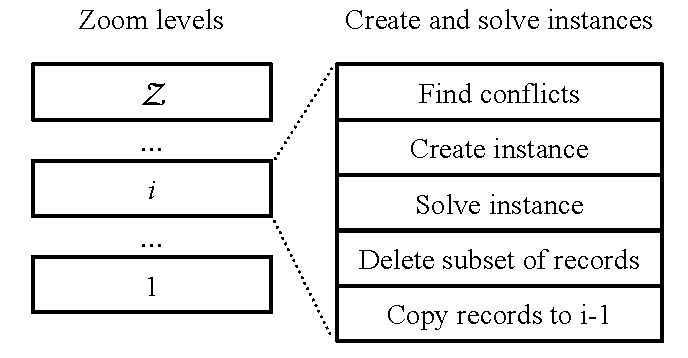
\includegraphics[scale=.6]{figs-cvl/cvl_stages.pdf}
\caption{Algorithmic framework: At each zoom level $i \in \{ 1, \ldots, \mathcal{Z} \}$ we solve a selection optimization problem. In the ladder approach, the problem is solved for the ``highest'' zoom level first.}
\label{fig:algorithmic-framework}
\end{center}
\end{figure}

Below we describe two different heuristic algorithms for solving the selection optimization problem. Let $n=|C|$ be the number of conflicts (or elements in the set multicover problem), and let $m=|R|$ be the number of records (or sets in the set multicover problem). Recall that $R_c \subseteq R$ is the set of records in conflict $c \in C$. The largest number of records in any conflict is $f = \max_{c \in C} |R_c|$, and is called the \emph{maximum frequency}.

\subsection{Static greedy algorithm (SGA)}
\label{sec:algorithms:sga}

In this algorithm, we consider each conflict $c \in C$ in turn, and simply choose the $\lambda_c$ records with minimum weight from the records $R_c$ --- independently of what has been chosen earlier. If the sets $R_c$ are disjoint, the algorithm is clearly optimal. However, in general no approximation guarantee can be provided. The algorithm runs in $O(n f \log f)$ time, as we just need to sort the records by weight for each conflict set; alternatively we can sort all records by weight in $O(m \log m)$ time and pick the minimum weight records from the conflicts in linear time in the total number of records in all conflict sets.

\subsection{LP-based greedy algorithm (LPGA)}
\label{sec:algorithms:lpga}

In this algorithm, we first solve a linear programming (LP) relaxation of the set multicover problem. This LP-problem is obtained by relaxing the constraint $x_r \in \{0, 1\}$ to $0 \leq x_r \leq 1$. Then we choose all records $r \in R$ for which the LP-solution variable $x_r$ is at least $1 / f$. Intuitively, we round up to 1 all fractional values that are large enough; the remaining fractional variables are rounded down to 0.

This algorithm provides a feasible solution to the selection optimization problem, and the approximation guarantee is $f$~\cite{vazirani2001approximation}; thus, if $f$ is small, the algorithm provides a good approximation guarantee. As the LP-problem can be solved in polynomial time, the complete algorithm is polynomial.


\section{Implementation}
\label{sec:implementation}

In this section, we describe how our implementation makes use of in-database execution to provide scalability and engine reuse for CVL (Section~\ref{sec:implementation:indatabase}). In addition, we discuss a number of extensions to CVL that we found to be useful for practical applications (Section~\ref{sec:implementation:extensions}). 

\subsection{In-Database Execution}
\label{sec:implementation:indatabase}

\minisec{Overview}
Since CVL is declarative, and CVL constraints are already expressed in SQL, it is natural to attempt to reuse as much existing DBMS technology as possible to execute CVL. Figure~\ref{fig:indatabase} shows how CVL is compiled for execution in a relational DBMS, which acts as the language runtime. The output of the CVL compiler is a database script for the target host, containing both SQL and stored procedures, and following the algorithmic framework of Figure~\ref{fig:algorithmic-framework}. The script is pushed down to the database engine, and operates against the appropriate input data stored in the system. This strategy offers us two main advantages:

\begin{enumerate}

\item Since all code is pushed down and both input and output reside in the database, we do not need to transfer any data outside of the database engine. This co-location of code and data is a significant advantage for large datasets.

\item By expressing as much as possible of the generated code in SQL, we can reuse decades of optimizations built into database engines, especially for geospatial data~\cite{Guttman1984:RTree,Hellerstein1995:GiST}. This opens up many opportunities, such as automatic optimization, parallelism, and selection of specialized algorithms and indexes.  

\end{enumerate} 

While the general strategy of compiling declarative languages to SQL has been pursued in other contexts, e.g., for XQuery~\cite{pathfinder} and LINQ~\cite{ferry}, our context poses a particular challenge of integrating the language with algorithmic solvers inside the database. 

\begin{figure}[htbp]
\begin{center}
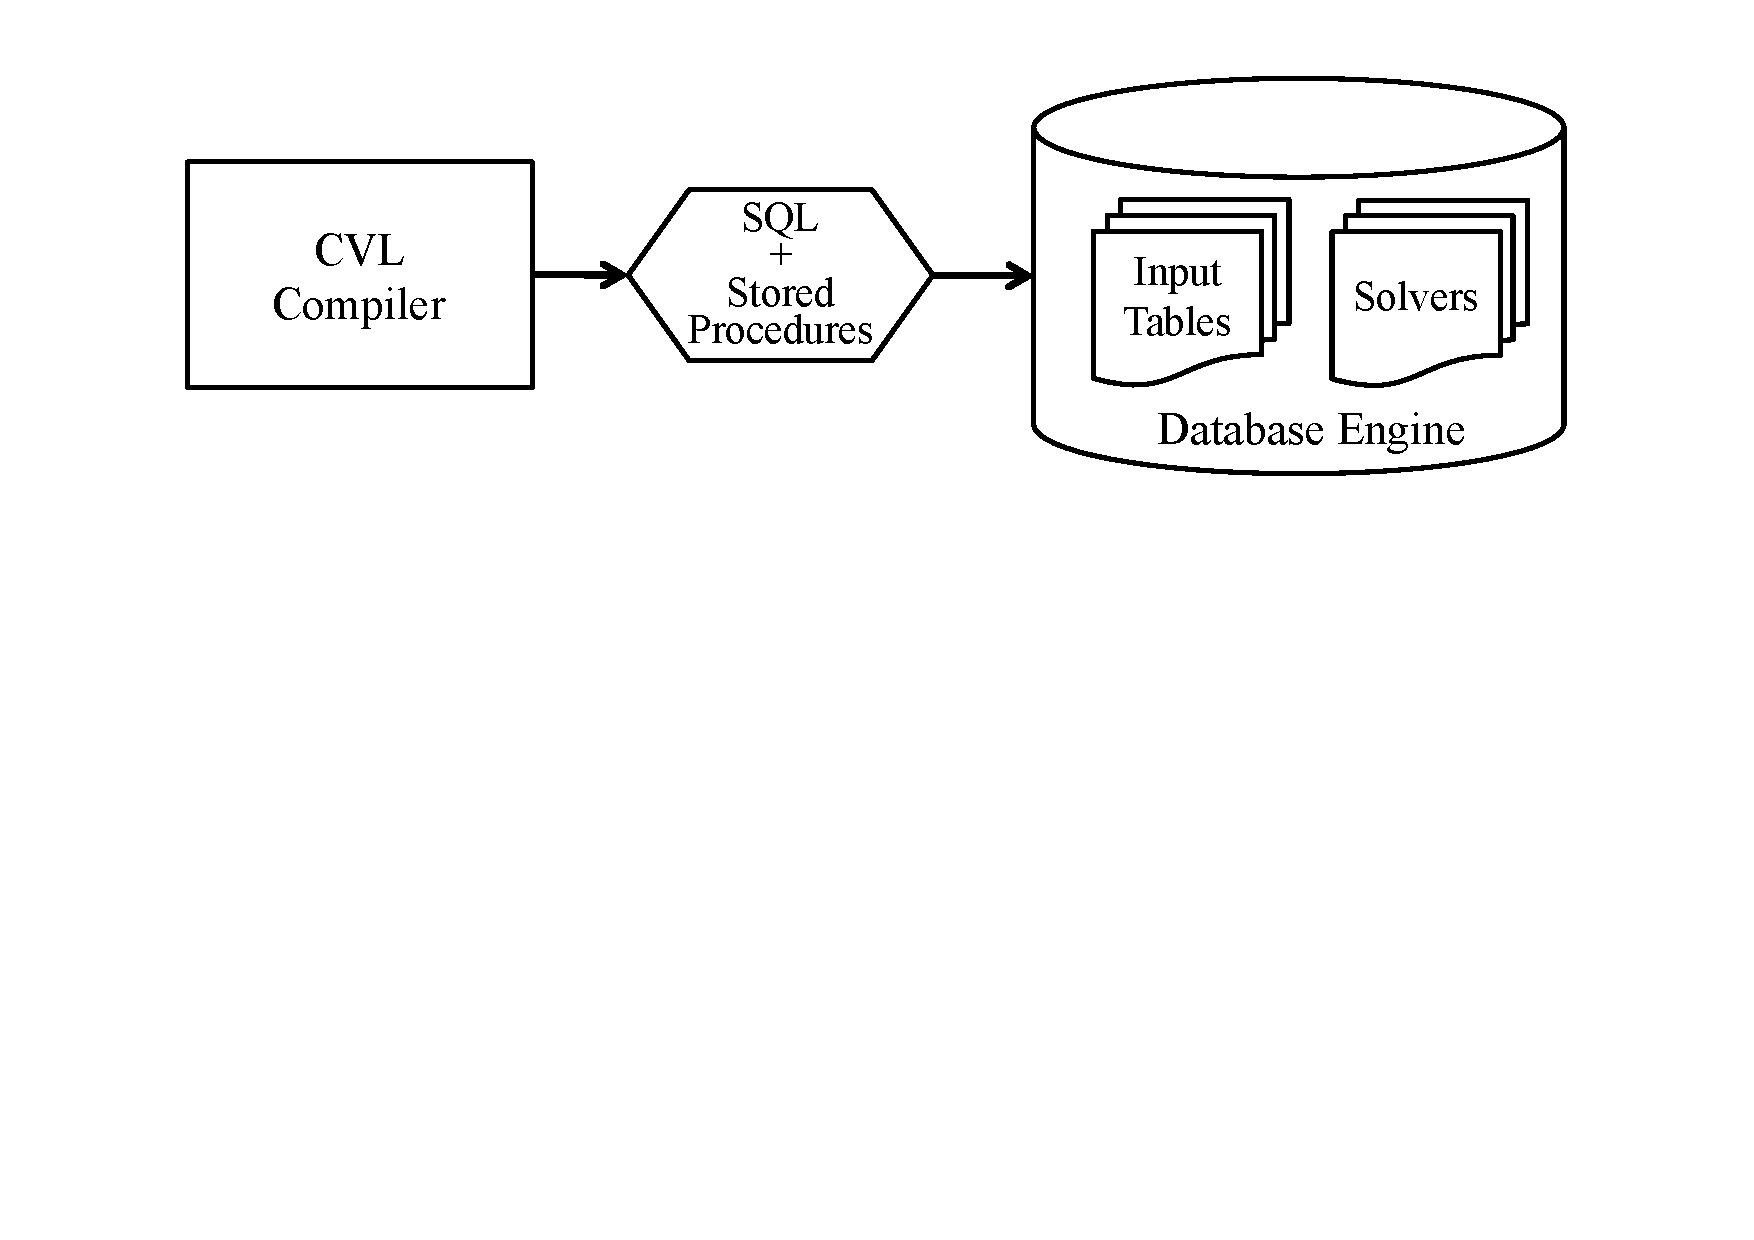
\includegraphics[scale=.35,viewport=400 375 450 550]{figs-cvl/indatabase-execution.pdf}
\caption{CVL and in-database execution.}
\label{fig:indatabase}
\end{center}
\vspace*{-1ex}
\end{figure}

\minisec{Solvers}
In Section~\ref{sec:cvl:algorithms}, we presented two different algorithmic approaches for solving CVL generalizations: static greedy (SGA) and LP-based greedy (LPGA). We now show how to express each of these approaches in SQL along with stored procedures. 

SGA is the simplest algorithm, and operates independently on the conflicts generated by each constraint. Suppose the conflicts $C$ generated by the active constraints are stored in a \emph{conflicts} table. Then SGA is tantamount to the query:

\begin{lstlisting}
SELECT rid
FROM (
  SELECT ROW_NUMBER() 
         OVER (PARTITION BY cid
               ORDER BY cvl_rank) AS r,
         rid, cvl_rank, lambda_c
  FROM conflicts) h
WHERE h.r <= h.lambda_c
\end{lstlisting}

For each conflict $c$, we order records by rank, and ensure that we pick at least $\lambda_c$ records. The declarative formulation allows us to reuse optimized sorting code in the database engine for execution.

LPGA solves a linear programming relaxation of the set multicover problem. We express LPGA by a stored procedure. The procedure accesses the conflicts for the constraints via SQL, constructs an appropriate LP, and then calls into an LP solver library. Since the solver library does not use built-in database optimizations, this execution strategy for LPGA only leverages the first advantage of data and code co-location listed above.

Finally, note that the code for finding conflicts is already expressed in SQL by the user for each constraint. As a consequence, this user code can make use of all built-in database optimizations available in the target engine.

\minisec{CVL runtime functions}
In the definition of the visibility constraint in Section~\ref{sec:cvl:create:constraint:statement}, we reference two stored procedures in the CVL runtime library, \texttt{CVL\_PointHash} and \texttt{CVL\_WebMercatorCells}. These functions are implemented in SQL and make use of the spatial extension of the database.

The procedure \texttt{CVL\_PointHash} uses a call to \texttt{ST\_GeoHash} to implement an injective mapping from points to strings. The GeoHash algorithm corresponds to a Z-order curve, and we exploit this for uniquely naming tiles when evaluating the visibility constraint, i.e. finding tiles with more than $K$ records.

The \texttt{CVL\_WebMercatorCells} function maps a geometry at a given zoom level to centroids of all intersected tiles (on that zoom level). We experimented with several ways to do this for general geometries (points, line segments, polygons) and found that rasterizing the geometry (using the function \texttt{ST\_AsRaster} in the spatial extension of the database) and iterating over the indices was the fastest for general geometries. For point records it is significantly faster to use the standard transformation function \texttt{ST\_SnapToGrid}.

%An improvement to \texttt{CVL\_WebMercatorCells} that we did not have time to implement is to compute tiles as quad-keys on the highest level only. Tile identifiers for lower levels are easily computed by taking prefixes of the quad-keys. This approach only benefits the running time when using constraints that are tile-based.

\subsection{Extensions}
\label{sec:implementation:extensions}

When designing CVL, we realized a number of interesting use cases for the language that we had not initially considered. This realization, along with our implementation experience of CVL use cases, led us to a set of extensions over the core language targeted at improving convenience of use. We present these extensions below.

\minisec{Partitioning and merging of datasets} 
A single input table may contain geospatial objects of different classes, e.g., roads and points of interest. When this is the case, users often wish to generalize some of these classes of objects independently, but obtain a single result map. While this can be done by merging the results of multiple GENERALIZE statements, we found it useful to add syntactic sugar to support this case. We extend the GENERALIZE statement with PARTITION BY and MERGE PARTITIONS clauses. PARTITION BY allows us to effectively segregate the input into multiple independent sets. MERGE PARTITIONS combines a few of these sets back together before providing them as input to generalization. For example, assume a \emph{geo\_objects} table contains highways, roads, restaurants, and hotels, tagged by a \emph{type} attribute. We could then generalize \emph{geo\_objects} as follows:

\begin{lstlisting}
GENERALIZE  geo_objects
TO network_and_poi_map
...
PARTITION BY type
MERGE PARTITIONS 'restaurant', 'hotel' 
              AS 'poi'
... 
\end{lstlisting}

In the example, we overlay independent generalizations of highways, roads, and points of interest into a single map. However, restaurants and hotels are generalized as a single input set.  

\minisec{Forced and all-or-nothing visualization}
Intuitively, constraints let users specify what is \emph{not} allowed in a given map, by forbidding the existence of conflicts. However, users also find it helpful to control certain behaviors that \emph{must} occur in their map. We extended the GENERALIZE statement with support for two types of behaviors: (1)~the ability to mandate a minimum zoom level for a particular partition of the input, and (2)~the ability to force that either all or none of the objects of a given partition be displayed. For example, a user may wish to specify that highways must only appear at zoom level 10 or lower in their map. In addition, for topological consistency, either the whole highway skeleton is displayed or no highways should show up. To achieve this goal, we extend the GENERALIZE statement by a FORCE clause with MIN LEVEL and ALLORNOTHING specifiers. Continuing the example above:

\begin{lstlisting}
...
FORCE MIN LEVEL 10 FOR 'highway' AND
ALLORNOTHING FOR 'roads'
... 
\end{lstlisting}

In the evaluation of CVL, the minimum level specifier controls what data is given as input for a zoom level. The all-or-nothing specifier, on the other hand, controls filtering of the output of the level generalization process. If the specifier is present, all records of a partition are deleted if any record from the partition input is not present in the output. By filtering output, we ensure that the result also respects all other constraints specified by the user. 

\section{Experimental Results}
\label{sec:experimental}

%\martin{Compare experimental results with theory e.g. expected approximation guarantee, number of constraints, number of records per constraint etc.}

In this section, we present experimental results with our implementation of CVL. Our experiments have the following goals:

\begin{itemize}

\item Evaluate the performance and solution quality of CVL generalizations with a variety of real-world datasets, including point data as well as complex shapes such as polygon and line data. 

\item Analyze the performance and solution quality of CVL generalizations produced under the proximity and visibility constraints presented in Section~\ref{sec:cvl:language} by both the SGA as well as the LPGA solvers of Section~\ref{sec:cvl:algorithms}.

\item Observe how the performance of CVL with different constraints and solvers scales with the number of objects in the geospatial dataset.

\end{itemize}

We start by presenting our experimental setup (Section~\ref{sec:exp:setup}), and then show results for both point data (Section~\ref{sec:exp:points}) and complex shapes (Section~\ref{sec:exp:complex:shapes}). Each result section discusses performance, quality, and scalability.


\subsection{Experimental Setup}
\label{sec:exp:setup}

\minisec{Datasets}
We have tested CVL using four real-world datasets, the largest of which containing 9 million points, and one synthetic dataset containing 30 million points. We list all datasets in Table~\ref{tab:cvl:datasets}. 

We have used three point datasets. The airports dataset is from Openflights and contains 7411 airports.\footnote{\url{http://openflights.org/data.html}} The tourism dataset contains 500 thousand points representing tourist attractions worldwide from the OpenStreetMap database.\footnote{\url{http://www.openstreetmap.org/}} The fractal dataset (synthetic) was created by iteratively copying and displacing points from the tourism dataset within a 10km radius until 30 million records were reached. We use this dataset for scalability experiments.

We have used two line datasets. The US rivers/streams dataset contains roughly 4 thousand rivers and roughly 27 thousand streams in the United States from the OpenStreetMap database. Records with identical name attributes have been merged into one. In the original dataset, most rivers are represented by multiple records, which is unfortunate in a selection situation (we wish to either select the waterway completely or not at all). 

We have used a single polygon dataset, the area information dataset from The Danish Natural Environment Portal, published by the Danish government.\footnote{\url{http://internet.miljoeportal.dk/}} This dataset contains 30 thousand high-fidelity administrative protection zone polygons, ranging from small polygons the size of buildings to large polygons the size of entire regions. The largest polygon has more than 36 thousand vertices.

%\minisec{Varying dataset size}
We have tested the scalability of CVL using both point and line datasets. A east-west unrolling approach is employed for gradually increasing the size of a dataset. First, we order records by x-coordinate, and then select increasingly larger prefixes of this order to derive larger datasets. The advantage of this approach over random sampling is that the spatial density of records is better preserved.

\begin{table}[htdp]
%\vspace{-2ex}
\caption{Datasets used in experiments}
%\vspace{-2ex}
\label{tab:cvl:datasets}
\begin{center}
\begin{tabular}{|c|c|c|c|c|}
\hline
\textbf{Origin} & \textbf{Dataset} & \textbf{Type} & \textbf{Records} & \textbf{Points} \\
\hline
Real & Airports & Points & $7K$ & $7K$ \\
Real & Tourism & Points & $500K$ & $500K$ \\
Synthetic & Fractal & Points & $30M$ & $30M$ \\
Real & US rivers & Line segments & $4K$ & $2M$ \\
Real & US rivers/streams & Line segments & $30K$ & $6M$ \\
Real & Proctection zones & Polygons & $30K$ & $9M$ \\
\hline
\end{tabular}
\end{center}
\label{default}
%\vspace{-2ex}
\end{table}%


\minisec{Hardware, software, and methods}
The machine used for testing was an Amazon EC2 instance with 17GB RAM, 2 x Intel(R) Xeon(R) CPU E5-2665 0 @ 2.40GHz and 20MB cache, running Amazon Linux 3.4.48-45.46.amzn1.x86\_64.\footnote{An image of the instance we used for testing is available through Amazon EC2 as an AMI. More information is available on the website for the project.}

The database used for testing was PostgreSQL 9.2.4 with PostGIS  2.0 built against the libraries GDAL 1.9.2 and GEOS 3.3.8. For the LP solver, we integrated the database with the convex optimization library CVXOPT version 1.1.6.\footnote{\url{http://cvxopt.org/}} We installed Python language bindings in the database against Python 2.6.8.

We ran each test three times on this installation, taking averages. We observed that measurements were very stable, with negligible difference in compute time between runs.

PostgreSQL always uses a single core to compute a transaction. Because the generalization process in CVL runs as a single long transaction, each job in CVL runs on a single core. A future direction would be to investigate parallel execution of CVL queries using a different language runtime such as a parallel database or a MapReduce environment.

\minisec{Average optimality ratio}
In our approach, we solve the multi-scale selection problem as a series of selection optimization problems. To get an indication of the solution quality, we compute for every selection optimization problem a lower bound using an LP-relaxation of the integer program. The numbers we present in Table~\ref{tab:points:overview} and Table~\ref{tab:complex:overview} include the average ratio between our solution value and the corresponding lower bound.


\begin{figure*}[tb]
  \begin{minipage}{0.329\linewidth}
    \centerline{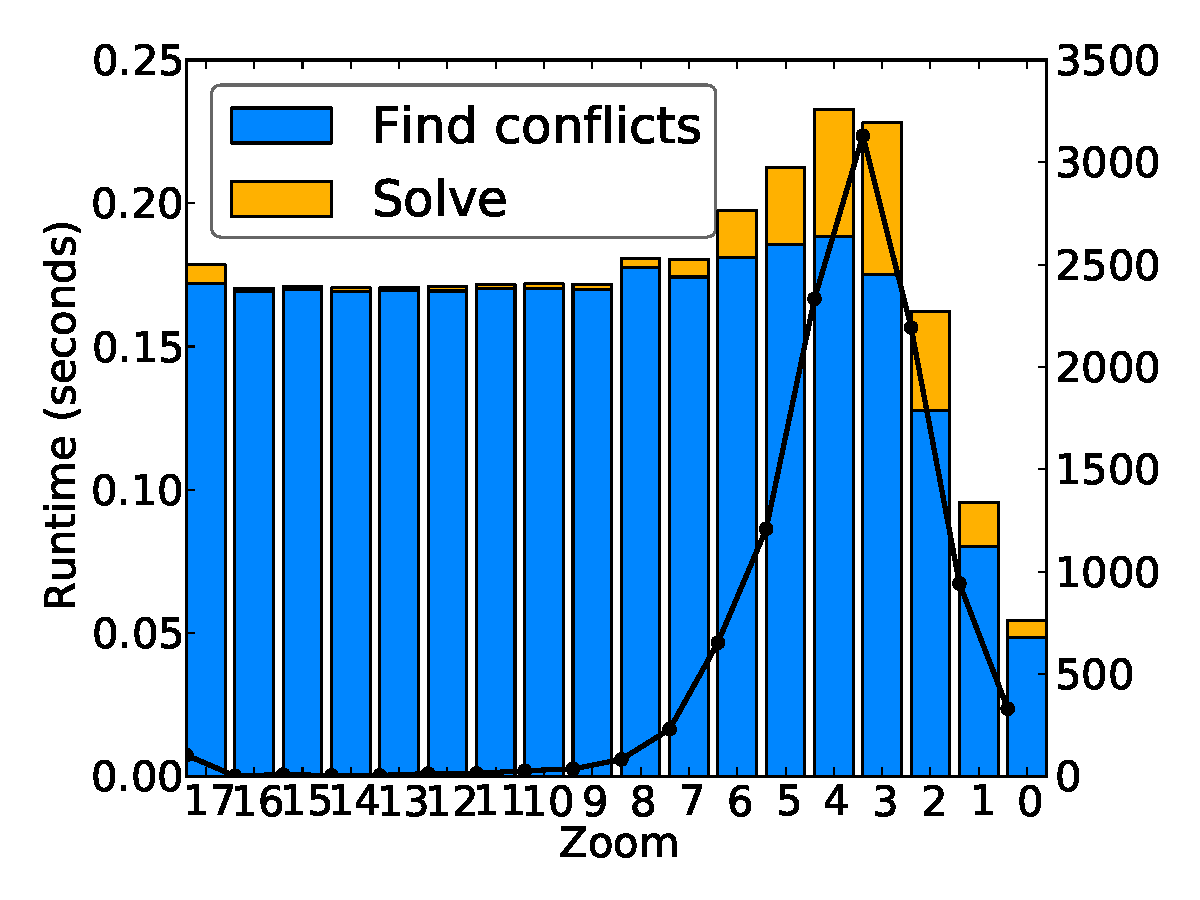
\includegraphics[width=0.9\linewidth]{./figs-cvl/prelim_pnt_7k_airports_heuristic_B.pdf}}
    \centerline{(a) SGA + Proximity}
  \end{minipage} \hfill
  \begin{minipage}{0.329\linewidth}
    \centerline{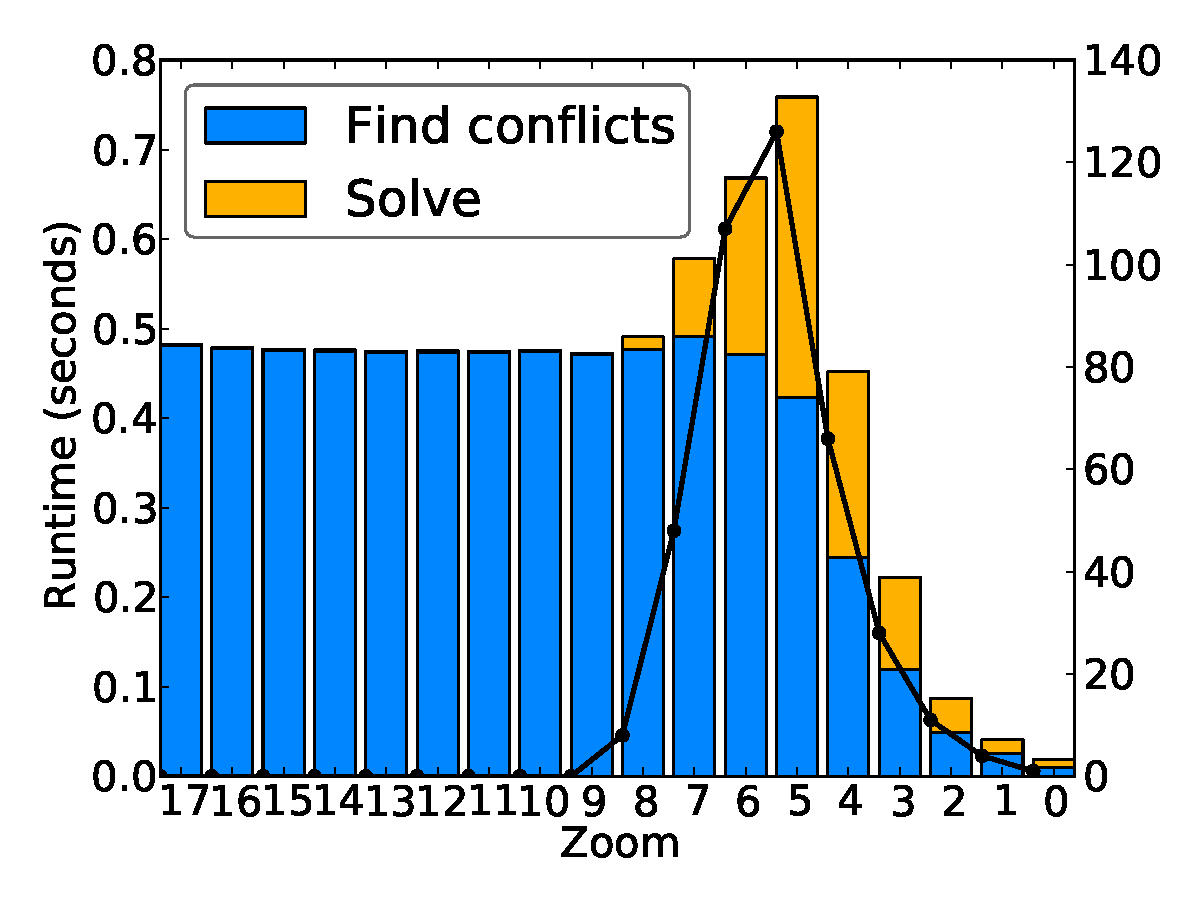
\includegraphics[width=0.9\linewidth]{./figs-cvl/prelim_pnt_7k_airports_lp_A.pdf}}
    \centerline{(b) LPGA + Visibility}
  \end{minipage} \hfill
  \begin{minipage}{0.329\linewidth}
    \centerline{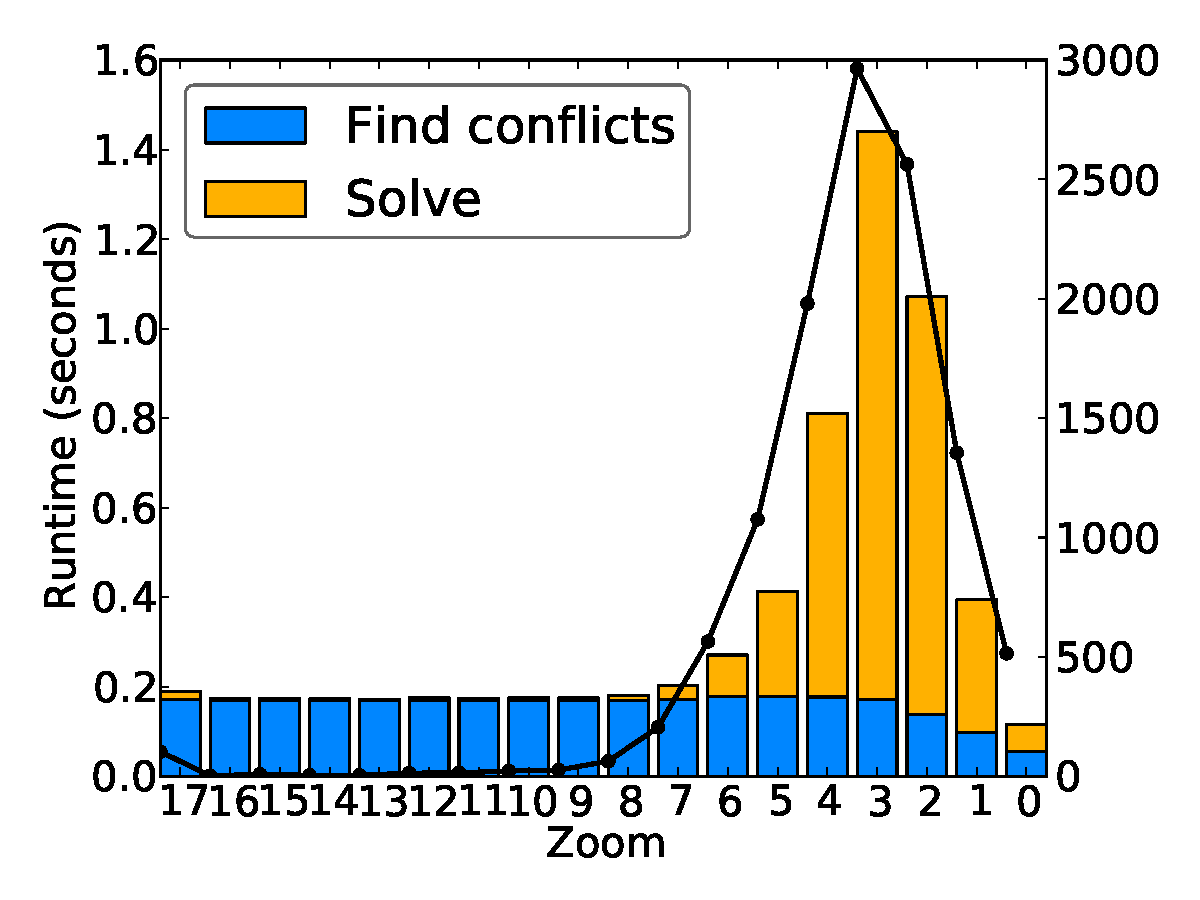
\includegraphics[width=0.9\linewidth]{./figs-cvl/prelim_pnt_7k_airports_lp_B.pdf}}
    \centerline{(c) LPGA + Proximity}
  \end{minipage}
%  \vspace{-1ex}
  \caption{Performance breakdown by zoom level, Airport dataset (7K points). The black line indicates number of conflicts} \label{fig:performance:airport}
%  \vspace{-2ex}
\end{figure*}

\subsection{Point Data}
\label{sec:exp:points}

In this section, we present experimental results with point datasets, namely the Openflight airports and the tourism datasets. We first discuss performance and quality for CVL and then proceed to analyze CVL's scalability behavior. Even though we experimented with all combinations of solvers (SGA / LPGA) and constraints (visibility / proximity / combined), we show only representative results for brevity. Results for the combined visibility and proximity constraints exhibited the same performance trends as of the most expensive of the two constraints. All other results followed similar trends as the ones explored below.



\begin{figure*}[tb]
  \begin{minipage}{0.329\linewidth}
    \centerline{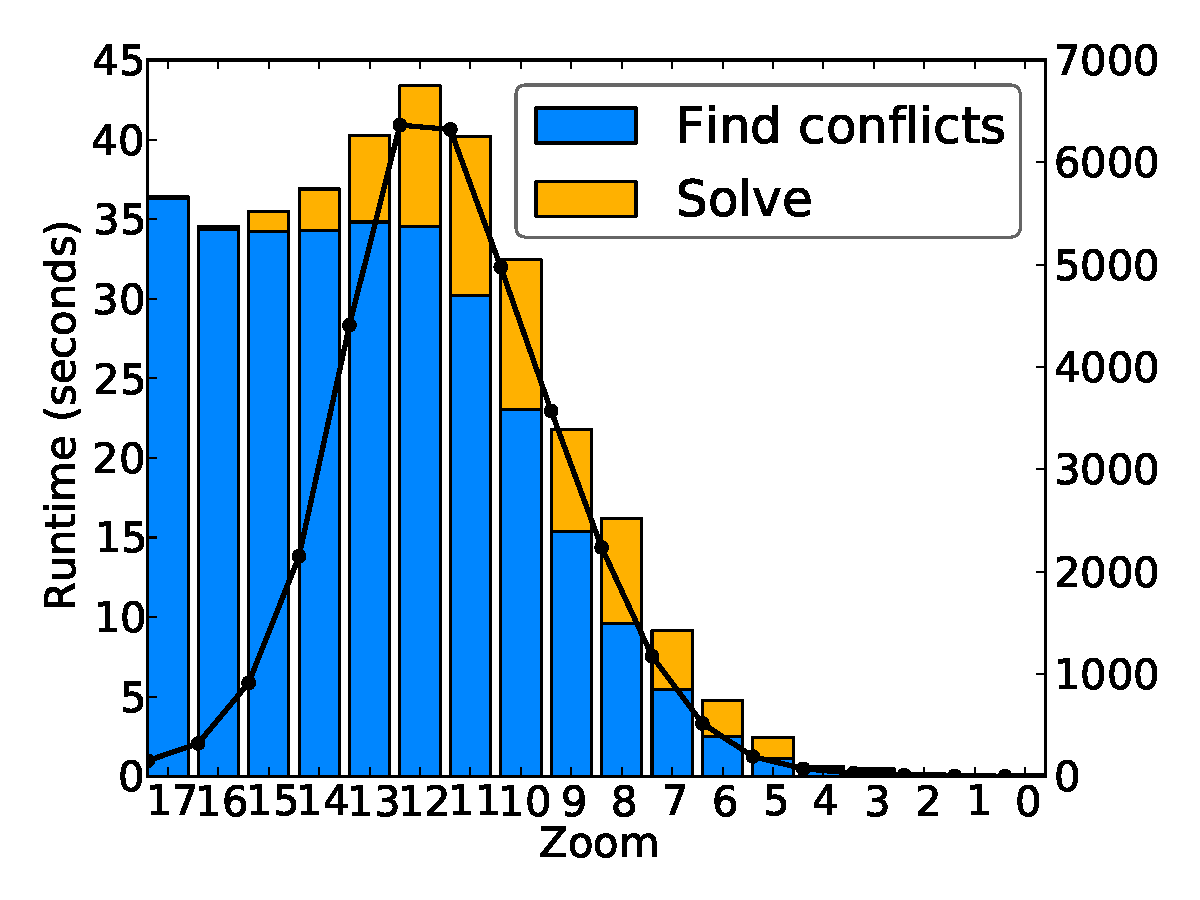
\includegraphics[width=0.9\linewidth]{./figs-cvl/prelim_pnt_500k_tourism_heuristic_A.pdf}}
    \centerline{(a) SGA + Visibility}
  \end{minipage} \hfill
  \begin{minipage}{0.329\linewidth}
    \centerline{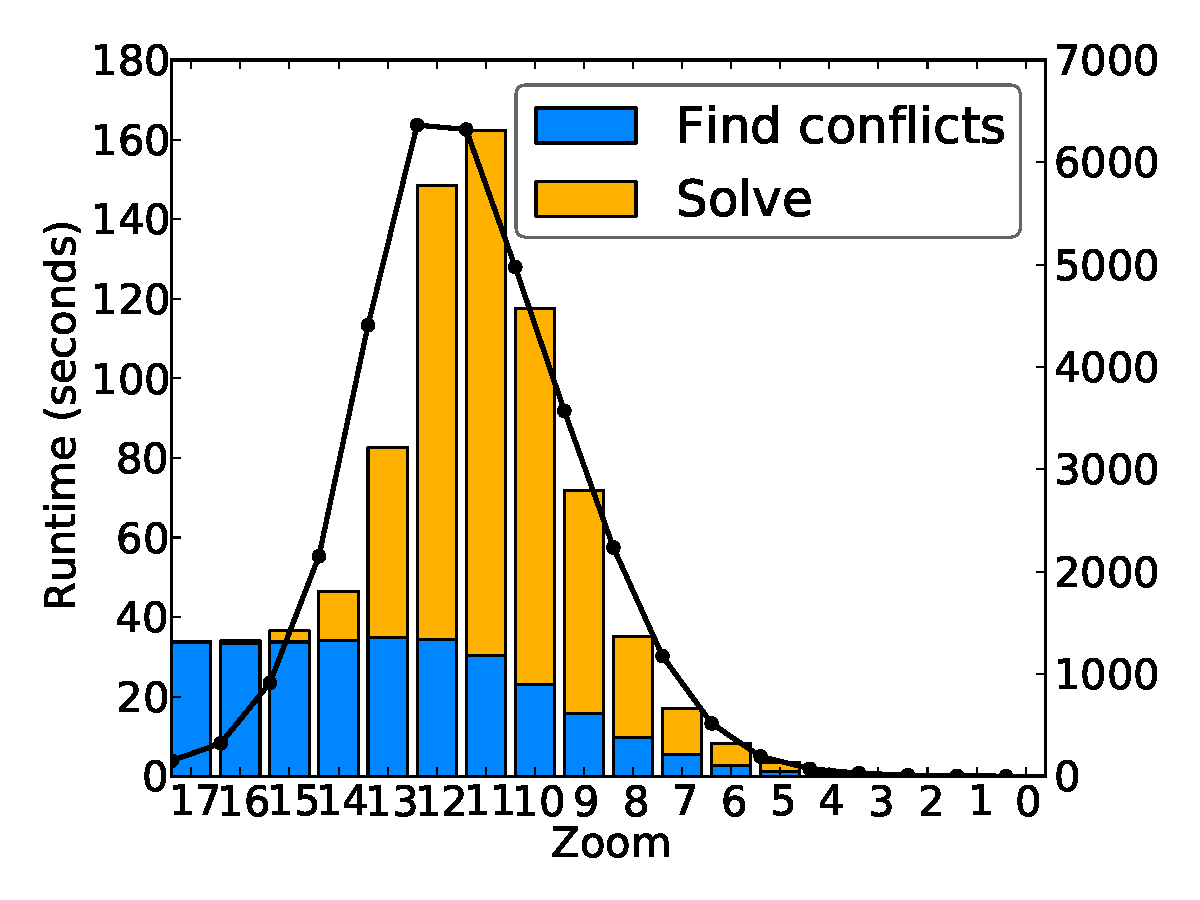
\includegraphics[width=0.9\linewidth]{./figs-cvl/prelim_pnt_500k_tourism_lp_A.pdf}}
    \centerline{(b) LPGA + Visibility}
  \end{minipage} \hfill
  \begin{minipage}{0.329\linewidth}
    \centerline{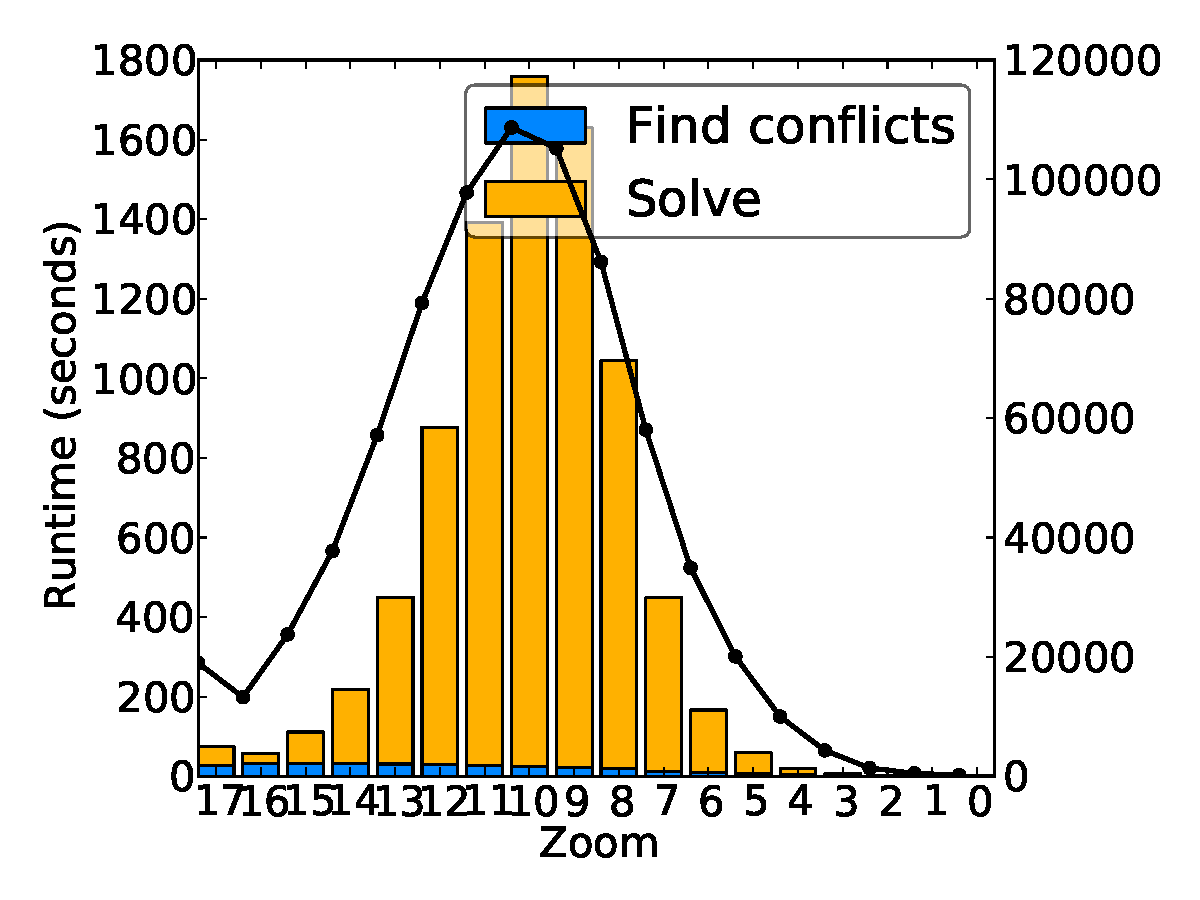
\includegraphics[width=0.9\linewidth]{./figs-cvl/prelim_pnt_500k_tourism_lp_B.pdf}}
    \centerline{(c) LPGA + Proximity}
  \end{minipage}
%  \vspace{-1ex}
  \caption{Performance breakdown by zoom level, Tourism dataset (500K points). The black line indicates number of conflicts} \label{fig:performance:tourism}
\vspace{-1ex}
\end{figure*}

\minisec{Overall performance and quality}
An overview of running times and solution qualities for the point datasets are shown in Table~\ref{tab:points:overview}. In Section~\ref{sec:algorithms:sga}, we remarked that SGA is optimal for disjoint conflict sets. This is confirmed by the entries for visibility + SGA in the table. For the point datasets we used for testing, the LPGA algorithm is also optimal or within $3\%$ of the optimum when combined with the visibility constraint, likely caused by the conflict sets being disjoint. Recall that the approximation guarantee of LPGA is $f$ (see Section~\ref{sec:algorithms:lpga}).

In terms of quality, the difference between SGA and LPGA is not stark for either constraint. The difference depends more on the constraint than on the solver, with visibility generally yielding the best solutions. However, the running time of SGA can be substantially shorter than that of LPGA. We analyze this effect in the following.

\begin{table}[htdp]
%\vspace{1ex}
\caption{Results for CVL on point datasets grouped by constraint}
%\vspace{-2ex}
\begin{center}
\begin{tabular}{|c|c|c|c|c|}
\hline
\textbf{Dataset} & \textbf{Constraint} & \textbf{Solver} & \textbf{Time} & \textbf{Avg. opt. ratio}\\ 
\hline
Airports (7K) & Visibility & SGA & 7s & 1.0 \\
Airports (7K) & Visibility & LPGA & 7s & 1.03 \\
Tourism (500K) & Visibility & SGA & 6m 9s & 1.0 \\
Tourism (500K) & Visibility & LPGA & 13m 35s & 1.0 \\
\hline
Airports (7K)  & Proximity  & SGA & 3s & 1.18 \\
Airports (7K)  & Proximity & LPGA & 7s s & 1.22 \\
Tourism (500K) & Proximity & SGA & 7m 17s & 1.21 \\
Tourism (500K) & Proximity & LPGA & 2h 18m & 1.24 \\
\hline
\end{tabular}
\end{center}
\label{tab:points:overview}
%\vspace{-2ex}
\end{table}%

\begin{figure*}[tb]
  \begin{minipage}{0.49\linewidth}
    \centerline{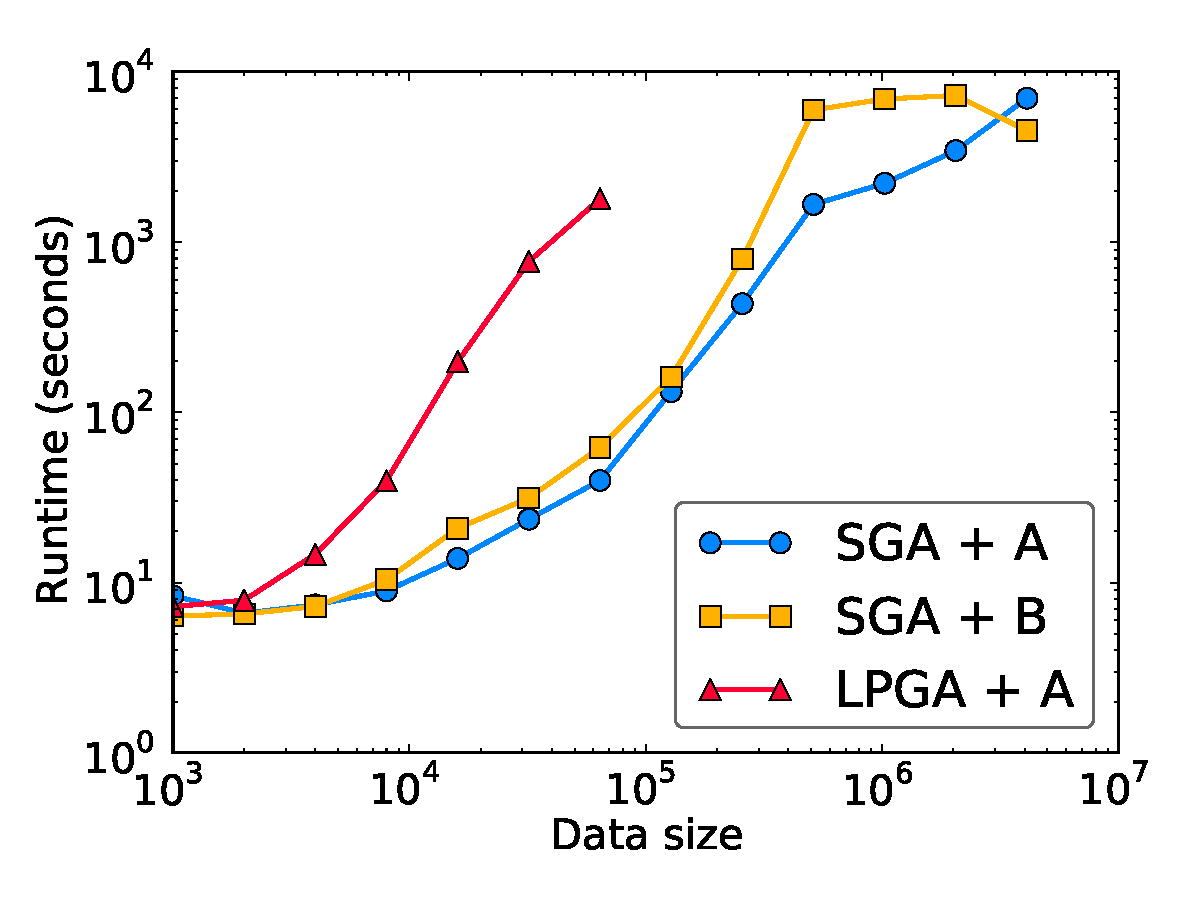
\includegraphics[width=0.75\linewidth]{./figs-cvl/scal_pnt_30m_synthetic.pdf}}
    \centerline{(a) Scalability for point data}
  \end{minipage} \hfill
  \begin{minipage}{0.49\linewidth}
    \centerline{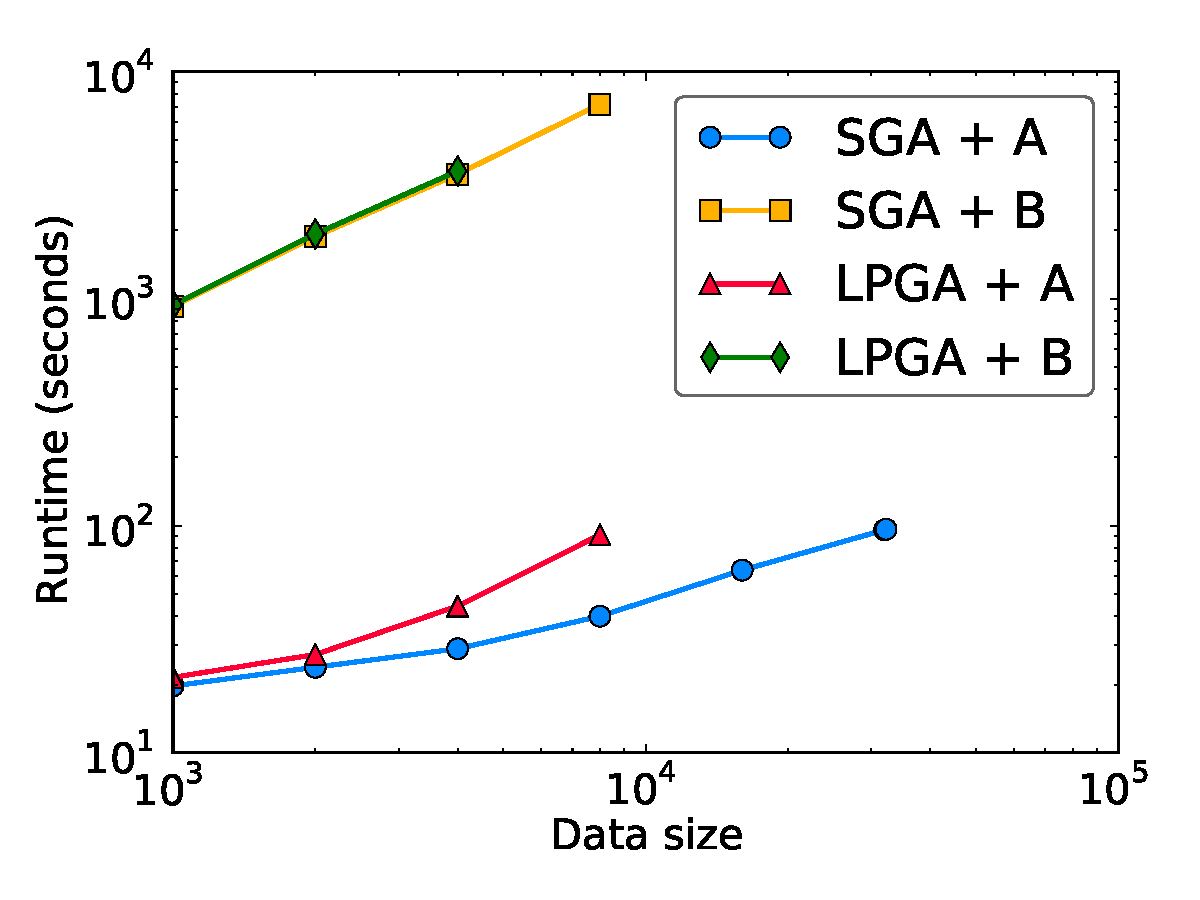
\includegraphics[width=0.75\linewidth]{./figs-cvl/scal_lin_30k_uswaterway.pdf}}
    \centerline{(b) Scalability for complex shape data}
  \end{minipage} \hfill
%  \vspace{-0ex}
  \caption{Scalability of CVL for point datasets and complex shape datasets. Constraints are marked as \emph{Visibility}: A, \emph{Proximity}: B} \label{fig:cvl:scalability}
%\vspace{-1ex}
\end{figure*}

\minisec{Performance breakdown}
Figure~\ref{fig:performance:airport} shows the performance breakdown per zoom level of executing CVL with the Openflight airports dataset. Note the different y-scales in the graphs. We have overlayed the number of conflicts per zoom-levels as a black line. In Parts~(a)-(c), we observe that the time needed to find conflicts is roughly stable until eight zoom levels, then slightly increases, and finally drops sharply for lower zoom levels. The constraints used generate few conflicts at higher zoom levels, given the relatively low density of the airport distribution in space. Nevertheless, even though almost no conflicts are generated, the dataset is still processed, resulting in roughly equal time for finding conflicts and negligible time for solving conflicts per zoom level. 
 
As zoom levels decrease, more conflicts naturally arise, leading initially to increased conflict finding time, as well as conflict solving time. However, as conflicts are solved, records are deleted from the dataset taken as input for the next zoom level. This procedure causes conflict finding time (and eventually total time) to drop significantly for low zoom levels. For SGA under the proximity constraint (Part (a)), total time at zoom level zero is over two times shorter than the initial runtime at zoom level 17; for LPGA under the visibility constraint (Part (b)), the difference in total time reaches over an order of magnitude.  

Conflict solving time does not increase equally for different solvers. SGA exhibits conflict solving time that is consistently smaller than LPGA. Peak total time for SGA under the proximity constraint (Part (a)) is roughly four times shorter than for LPGA (Part (c)). In addition, LPGA is extremely sensitive to the number of conflicts reported by user-defined constraints. From Parts (b) and (c), we can see that LPGA exhibits peak conflict solving time over three times larger for the proximity constraint than for the visibility constraint, since the latter generates far fewer conflicts than the former.

Figure~\ref{fig:performance:tourism} exhibits results with the larger tourism attraction dataset. Since the dataset is denser in space than the airport dataset, conflicts are found and solved at higher zoom levels, resulting in an earlier drop in total time per zoom level. For Parts (a)-(c), total time is uninteresting for zoom levels lower than five. The same cannot be said, however, about peak total time in general, and about conflict solving time in particular.

Parts (a) and (b) compare performance of SGA and LPGA under the visibility constraint. Even though visibility generates a smaller number of conflicts than proximity, peak total time for LPGA is still roughly a factor of four larger than for SGA (see zoom level 11). Note that the difference is completely due to the efficiency of the solver, since the time to find conflicts is essentially the same for both methods. Total time for LPGA rises prohibitively when we employ the proximity constraint, reaching a baffling peak of near half an hour at zoom level 10 (Part (c)). While not shown, total times per zoom level for SGA under the proximity constraint are roughly comparable to the times reported in Part (a) for the visibility constraint using this dataset. SGA's peak total time is slightly above 40 seconds, roughly a factor of 40 smaller than LPGA's.         

In summary, and as discussed in Section~\ref{sec:algorithms:sga}, SGA performs significantly better than LPGA, but it does not do so at the cost of quality, at least for point datasets.

%While SGA performs significantly better than LPGA, it does not do so at the cost of quality, at least for point datasets. As discussed in Section~\ref{sec:algorithms:sga}, SGA is optimal for the visibility constraint, since conflict sets are disjoint. For the proximity constraint, we observe that the solutions have comparable quality for the two algorithms, while the running time of LPGA is much larger than SGA, and more so for the larger dataset.

\minisec{Scalability}
We tested the scalability of CVL by varying the size of the synthetic dataset of 30 million points, starting with one thousand records, and tested by iteratively doubling up until we reached roughly four million records. We scaled the dataset with the sweep-line approach introduced in Section~\ref{sec:exp:setup}. We plot the running time of each solver/constraint combination for different dataset sizes in Figure~\ref{fig:cvl:scalability}.

In general, SGA scales far better than LPGA with the number of objects, confirming the observations from the performance breakdown above. After reaching four million points the running time became prohibitively large (more than 3 hours) even for SGA. Up to this point, the algorithm scales roughly linearly. The running time of the solvers depends on the number of conflicts, as well as on the structure of the conflicts. It is easy to see that after the first zoom-level, the number of conflicts is bounded by a constant that is proportional either to the number of records (for the proximity constraint) or the number of cells (for the visibility constraint). For the proximity constraint, the number of conflicts is bounded due to circle packing. For the visibility constraint, each cell can contain at most $64$ records for $K=16$, after the first zoom-level is processed. This is because each cell contains only records from four cells on the previous (higher) zoom-level, each of which contains only 16~records.

%There is a curious fall in running time for SGA with the proximity constraint. We did not gather sufficient data during the scalability experiment to explain this phenomenon.


\subsection{Complex Shape Data}
\label{sec:exp:complex:shapes}

\minisec{Overall performance and quality}
In Table~\ref{tab:complex:overview} we summarize running times and average optimality ratios for complex shape data. We immediately observe that LPGA is now consistently better than SGA with regard to solution quality. This is in contrast to what we saw for points. We believe the cause to be that the conflict sets are no longer disjoint, and SGA suffers from this.

\begin{table}[htdp]
\caption{Results for CVL on complex datasets grouped by constraint}
%\vspace{-1ex}
\begin{center}
\begin{tabular}{|c|c|c|c|c|}
\hline
\textbf{Dataset} & \textbf{Constraint} & \textbf{Solver} & \textbf{Time} & \textbf{Avg. opt. ratio}\\ 
\hline
Rivers (4K) & Visibility & SGA & 1h 32m & 1.36 \\
Rivers (4K) & Visibility & LPGA & 1h 33m & 1.0 \\
Zones (30K) & Visibility & SGA & 13m 38s & 1.20 \\
Zones (30K) & Visibility & LPGA & 32m 15s & 1.14 \\
\hline
Rivers (4K)  & Proximity  & SGA& 1h 11m s & 1.46 \\
Rivers (4K)  & Proximity & LPGA & 1h 31m & 1.11 \\
Zones (30K) & Proximity & SGA & 4h 28m & 1.72 \\
Zones (30K) & Proximity & LPGA & --- & --- \\
\hline
\end{tabular}
\end{center}
\label{tab:complex:overview}
%\vspace{-2ex}
\end{table}%

\begin{figure*}[tb]
  \begin{minipage}{0.329\linewidth}
    \centerline{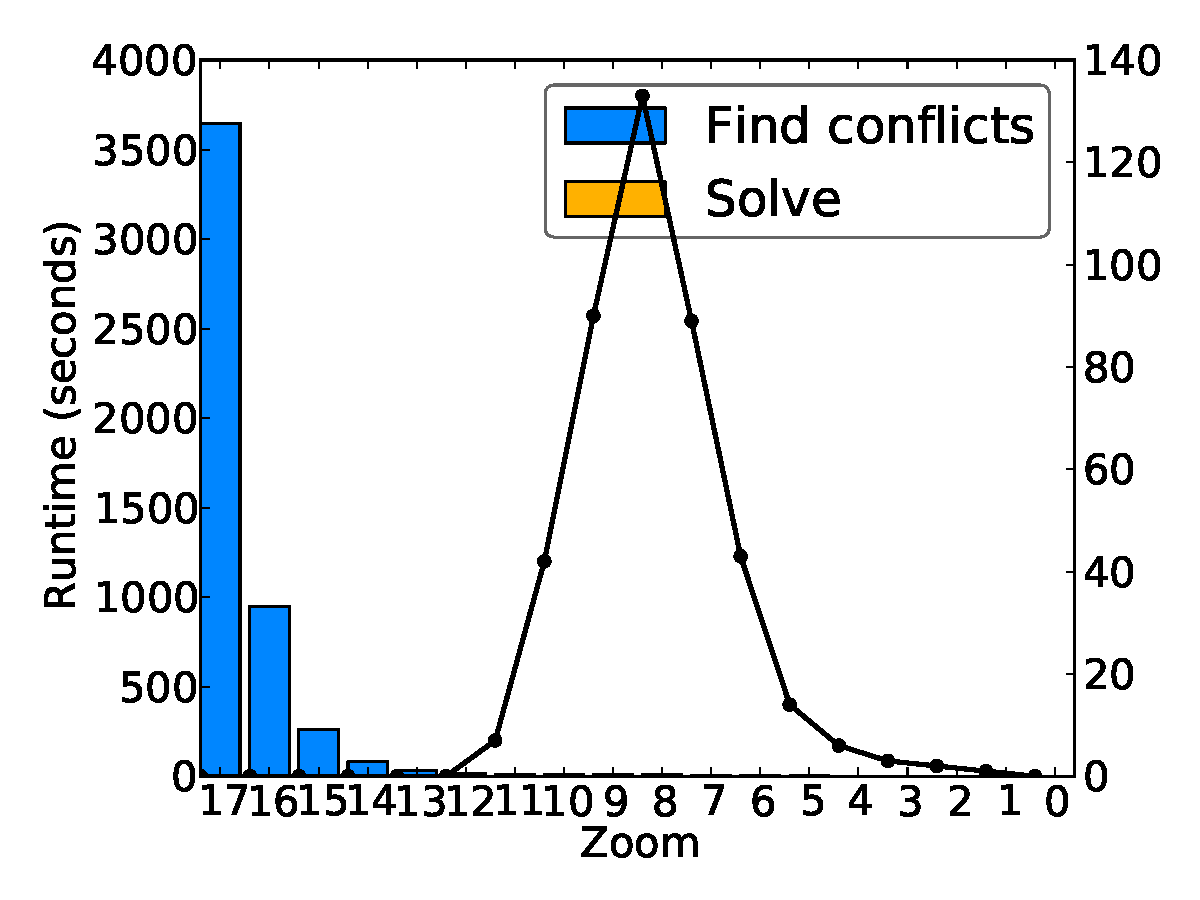
\includegraphics[width=0.9\linewidth]{./figs-cvl/prelim_lin_30k_uswaterway_lp_A.pdf}}
    \centerline{(a) LPGA + Visibility}
  \end{minipage} \hfill
  \begin{minipage}{0.329\linewidth}
    \centerline{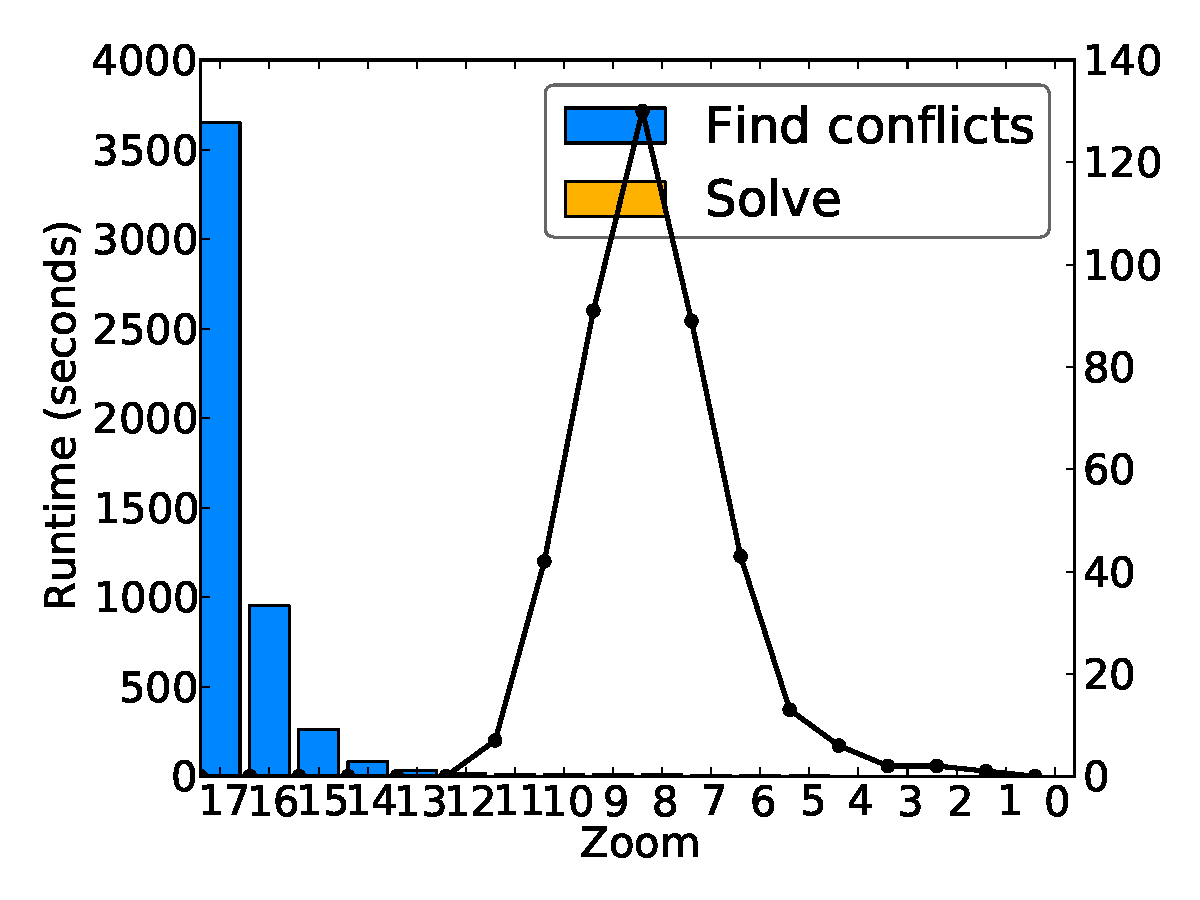
\includegraphics[width=0.9\linewidth]{./figs-cvl/prelim_lin_30k_uswaterway_heuristic_A.pdf}}
    \centerline{(b) SGA + Visibility}
  \end{minipage} \hfill
  \begin{minipage}{0.329\linewidth}
    \centerline{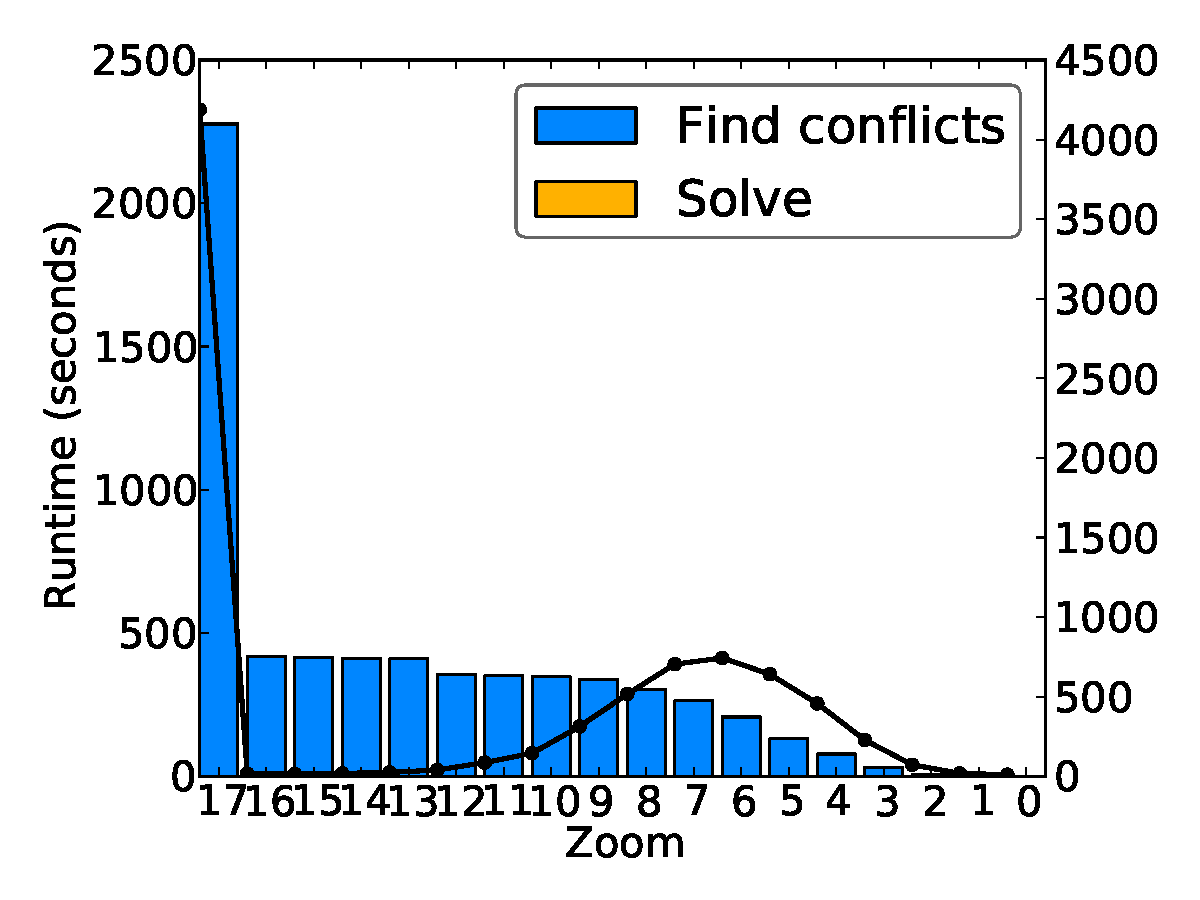
\includegraphics[width=0.9\linewidth]{./figs-cvl/prelim_lin_30k_uswaterway_lp_B.pdf}}
    \centerline{(c) LPGA + Proximity}
  \end{minipage}
%  \vspace{-1ex}
  \caption{Performance breakdown by zoom level, Rivers dataset (4K records). The black line indicates number of conflicts} \label{fig:performance:complex}
%\vspace{-2ex}
\end{figure*}


\minisec{Performance breakdown}
In Figure~\ref{fig:performance:complex}, we show three performance breakdowns for the Rivers dataset. We make two observations. First, the running time is now completely dominated by finding conflicts. This is because the complexity of finding conflicts depends on the fidelity of the geometries that are compared. 
%For the proximity constraint, the complexity is proportional to the product of point counts for the two geometries compared in the distance test. For the visibility constraint, the complexity depends on the number of tiles occupied by each geometry, which depends on either the length or the area of the geometry. The solving time does not directly depend on the geometric properties, only on the number and structure of conflicts.
Parts (a)-(c) illustrate the effect in more detail, with Part (a) in particular showing the breakdown of a solution with an average optimality ratio of $1.0$. We see that for complex shape datasets, the running time is mostly dominated by the time spent finding conflicts. Since finding conflicts operates over the geometric properties of the data, it requires time proportional at least to the number of points that make up each complex shape. When solving conflicts, the running time is independent of geometric complexity. Interestingly, the time necessary to find conflicts is so high that it shadows the negative effect that a larger number of conflicts has on the conflict resolution time of LPGA (compare with Section~\ref{sec:exp:points}).

%This causes the running time to be dominated by finding conflicts for complex shape datasets. The LPGA solver is the exception when many conflicts are reported. A similar effect was seen for points, indicating that the LPGA solver does not scale well with the number of conflicts. %, which is confirmed in our scalability experiments.

\minisec{Scalability}
In Figure~\ref{fig:cvl:scalability}(b), we show scalability results for complex shape data. Here scalability depends more on the choice of constraint than on the choice of solver. The proximity constraint scales much worse than the visibility constraint with the number of objects. This is because the running time of the distance test used in the proximity constraint is proportional to the product of point counts in the two geometric shapes used in each comparison. In contrast, evaluating the visibility constraint depends on the number of tiles that each shape intersects, which depends more on the length or area of each shape. 

While constraints matter more to scalability for complex shapes than for point data, the SGA solver scales better than LPGA with number of objects, which was also the case for the point datasets examined in Section~\ref{sec:exp:points}.

\section{Related work}
\label{sec:cvl:related:work}

Cartographic generalization is a classic topic of investigation in the GIS community, and several models have been developed for generalization operations~\cite{harrie2007modelling}. While the problem has been considered by some as AI complete~\cite{frank1994multiscaletree}, recent work has focused on automatic map generalization based on optimization models or queries for filtering~\cite{sarma2012fusiontables,nutanong2012multiresolution}. This reduction in scope reflects the need of providing a wide variety of web-accessible maps summarizing ever increasing amounts of geospatial datasets. Our work provides support for the same trend.  

The optimization approach of Das Sarma et al.~\cite{sarma2012fusiontables} is the most related to our work. In contrast to our approach, however, Das Sarma et al. do not provide a flexible declarative interface for user-defined constraints, nor does their approach leverage SQL. 
%As a consequence, their approach is restricted to memory-resident datasets and pre-specified, not user-defined, constraints. 
In addition, it is hard to integrate their approach with existing geospatial data serving infrastructures, which are mostly based on standard spatial database technology.

User-defined constraints and declarative specifications have been shown to yield elegant solutions to a variety of problems in data management, including record deduplication~\cite{ArasuRS09:Dedupalog}, database testing~\cite{BinnigKL07:ReverseQP,Binnig:2007:SymbolicQP}, as well as cloud and networking resource optimization~\cite{Liu:2012:Cologne}. Our work brings these ideas to the context of map generalization and geospatial data, and as mentioned previously, is among the first frameworks to implement the vision of reverse data management~\cite{meliou2011reverse}. 

In-database processing has also been explored successfully in diverse contexts in the literature. Translation of high-level languages, such as XQuery or LINQ, to SQL lead to highly scalable and efficient implementations~\cite{pathfinder,ferry}. A number of recent approaches have targeted expressing complex statistical analytics in SQL~\cite{Hellerstein:2012:Madlib,Ordonez2007:StatisticsUDFs}. In contrast, we show how in-database processing can be used in the implementation of a declarative language for map generalization which includes solvers and constraints, leveraging the trend to incorporate whole programming language interpreters and support for spatial data structures in database engines~\cite{Blakeley2008:DotNET}.  

Our approach dovetails with a number of techniques from the literature, which hold potential to further extend or complement it. First, we observe that the running time of the LP-based greedy algorithm (LPGA) is generally high. We implemented this algorithm because it provides a theoretical bound on the solution quality. We plan to explore other algorithms for set multicover, such as the greedy algorithm described by Rajagopalan and Vazirani~\cite{rajagopalan1998primal}, to improve running time compared to the LP-based greedy algorithm, while achieving good quality. An interesting challenge is how to express such algorithms entirely in SQL.

Second, this work considers only selection of objects. An important extension is to allow other data reduction operations, such as geometric transformation and aggregation of objects. While we believe that CVL could be adapted to these additional requirements, this would imply modeling alternative semantics and procedures for satisfying constraints in our framework.

Third, we would like to experiment with geospatially-aware parallel processing infrastructures, such as Hadoop-GIS~\cite{Aji:2013:HadoopGIS}, for even further scalability in computing map generalizations. Finally, once a map generalization is complete, the resulting map must be served to end-users. This problem is orthogonal to our work, and classic linearization techniques can be applied~\cite{hilbert1891ueber}. All of these are interesting avenues for future work.


In this paper, we present a novel declarative approach to the data reduction problem in map generalization. 
%The proposed approach is complete in the sense that it integrates seamlessly with existing database and cartographic generalization technology. 
The proposed approach integrates seamlessly with existing database technology, and allows users to specify, using the proposed CVL language, and across all scales, what goals and constraints the generated map should fulfill --- leaving the detailed selection decisions to the system. The system leverages an algorithmic mapping which enables at the same time user-defined constraints and reuse of methods from the optimization literature. Our experiments show that the approach performs well for off-line processing and produces maps of high quality.



\chapter{Glossy: Global Selections for Data Visualizations}
\label{chapter:glossy}
\lstset{
  language=sql
}


\section{Introduction}
\label{sec:glossy:introduction}

We are faced with unprecedented data volumes in organizations across a wide variety of sectors~\cite{MCB+11:McKinsey}. In this context, data visualization of large and complex data is attracting renewed attention in data management and visual analytics~\cite{FeketeS12:DMVisChallenges,hanrahan:enthusiast,wu:case}. Computational journalism~\cite{CohenHT:2011:CompJournalism}, data science~\cite{KandelPHH12:InterviewStudy}, and citizen activism~\cite{ViegasM:2009:ManyEyes} are just a few examples of the new types of applications that require visualizations to help humans make sense of large datasets. To support these applications, it is crucial to abstract data in a way that reduces its volume, given that the amount of pixels in a display is often insufficient to convey detailed information about a large dataset.

Two of the most intuitive data reduction operations are to aggregate or select data. Data aggregation provides insights into the characteristics of datasets as a whole; however, this overview comes at the price of potentially losing valuable detail. Data selection, on the other hand, allows users to examine particular examples to get a more nuanced understanding of the data; however, this detail comes at the price of potentially being overwhelming. Recent studies indicate that data scientists find it difficult to express information needs for visualizations in existing query and programming languages, creating a substantial gap to be closed in current technology~\cite{KandelPHH12:InterviewStudy}.
 
\begin{figure*}[!t]
     \begin{minipage}{0.62\linewidth}
        \centerline{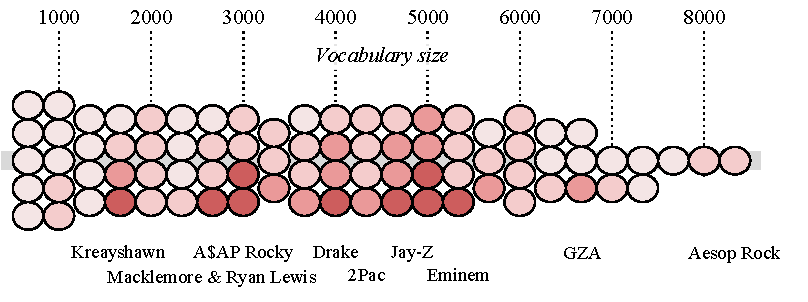
\includegraphics[width=0.99\linewidth]{figs-glossy/rappers_viz.pdf}}
        \vspace{-1ex}
        \caption{A visualization of rappers according to their vocabulary requires selecting the most popular rappers for each word bracket out of a much larger set of artists. The visualization should display more rappers as we zoom into word brackets for more detail. Note that even though the visualization organizes rappers in a word line (1-D), it uses the popularity dimension of the artist to both aid selection and to shade the surviving bubbles.}\label{fig:example:rappers}
    \end{minipage} \hfill
       \begin{minipage}{0.36\linewidth}
        \centerline{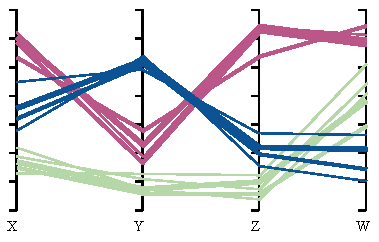
\includegraphics[width=0.99\linewidth]{figs-glossy/parallel_coordinates.pdf}}
        \vspace{-1ex}
        \caption{A visualization of k-means clusters with parallel coordinates requires us to limit to $n$ the number of lines that can cut through each dimension line segment for any vertical unit of space, at a scale-dependent resolution. Line widths are set by distances to cluster centers.} \label{fig:example:clusters}
    \end{minipage} \hfill
\end{figure*}
\begin{figure*}[!t]
     \begin{minipage}{0.62\linewidth}
        \centerline{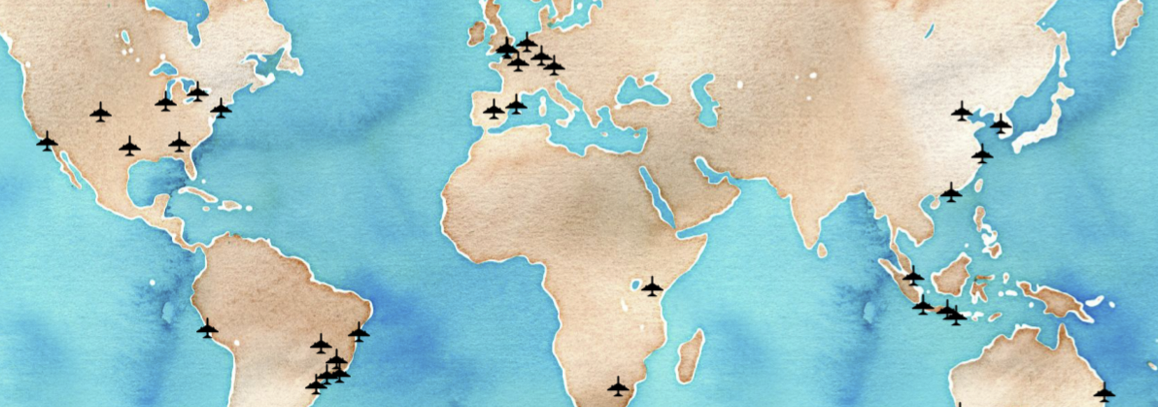
\includegraphics[width=0.99\linewidth]{figs-glossy/airports.png}}
        \vspace{-1ex}
        \caption{A visualization of airports in a geographical map requires the selection of the airports with the most traffic out of a larger set of airports. The visualization should display more airports as we zoom into geographical regions for more detail.}\label{fig:example:airports}
    \end{minipage} \hfill
       \begin{minipage}{0.36\linewidth}
        \centerline{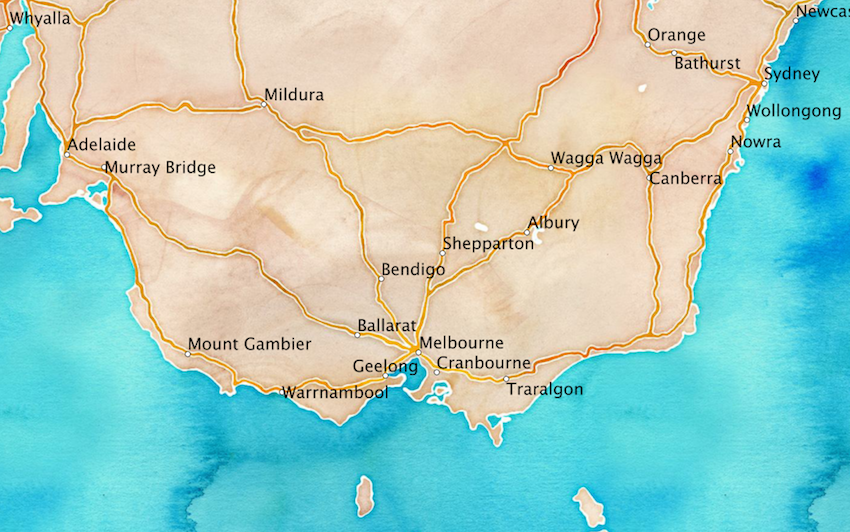
\includegraphics[width=0.96\linewidth]{figs-glossy/placenames_viz.png}}
        \vspace{-1ex}
        \caption{A visualization with placenames in a geographical map requires displaying or omitting labels according to scale.} \label{fig:example:placenames}
    \end{minipage} \hfill
\end{figure*}
 
Despite the wealth of existing work on data visualization, most systems have either focused on abstracting data by aggregation~\cite{blais:generating,LinsKS13:Nanocubes,StolteTH:2003:Multiscale,vartak:seedb}, or on devising techniques to squeeze a whole dataset into the available pixels~\cite{KeimK95:VisDB,KruskalW78:MDS}. The problem of creating visualizations that explicitly show representative items from a large underlying dataset has received far less attention. Nevertheless, the importance of this problem is significant. Figures~\ref{fig:example:rappers} to~\ref{fig:example:placenames} illustrate a few visualizations that crucially depend on data selection. These visualizations vary substantially in dimensionality, going from a single axis in the case of Figure~\ref{fig:example:rappers} to a parallel coordinates plot of multiple dimensions in Figure~\ref{fig:example:clusters} to two-dimensional geographical maps in Figures~\ref{fig:example:airports} and~\ref{fig:example:placenames}. Furthermore, these visualizations employ multiple scales to allow users to zoom into the data and see more records from the underlying dataset in an interactive fashion. Moreover, these visualizations are becoming ever more necessary for human understanding as we move towards an age of large datasets and data enthusiasts~\cite{hanrahan:enthusiast,markl:breaking}. Even though previous work has targeted particular examples of such visualizations, e.g., for spatiotemporal data~\cite{jugel:m4,KefaloukosSZ14:CVL,DasSarmaLGMH12:FusionTables}, a generic solution to multi-scale data selection has remained elusive. Such a solution should ideally be able to globally sample records, while respecting user-defined constraints and notions of record importance, and at the same time elegantly reuse database technology to operate on large datasets.   


In this paper, we introduce Glossy (GLObal Selection SYstem), a system that computes global selections over records stored in an RDBMS. In short, Glossy's novelty and utility rests on three pillars: (a) Glossy SQL, an extension of SQL that allows visualization developers to express global selection in a concise, yet familiar, query language, (b) an efficient translation of Glossy SQL into pure SQL, which allows Glossy to harness the power of mature query optimizers and indexed tables at runtime, (c) support for global selection over any type of tabular data, not just data within a certain domain (e.g., temporal or spatial data). With Glossy, multi-scale global selections of data for all the visualizations in Figures~\ref{fig:example:rappers}--\ref{fig:example:placenames} can be achieved concisely in a common declarative framework.  

\subsection{Our Contributions}

Having set the stage for our work above, we start by reviewing related approaches (Section~\ref{sec:glossy:related:work}). Then, the paper presents its main contributions:

\begin{enumerate}

\item Motivated by a wide range of use cases in data visualizations (Section~\ref{sec:use:cases}), we introduce Glossy SQL, an extension of SQL centered around the notion of global selections. We show how Glossy SQL can be used to declaratively express global selections for visualization use cases, as well as formally define single-scale and multi-scale global selections (Section~\ref{sec:global:selections}).  

\item Given a well-grounded understanding of the semantics of global selection, we proceed to present a translation of Glossy SQL into pure SQL. This translation allows for immediate use of Glossy SQL over existing RDBMS. In addition, it also allows Glossy to efficiently and scalably process global selection queries by reusing mature query processing technology (Section~\ref{sec:sql:translation}). 

\item In a set of experiments (Section~\ref{sec:experimental:evaluation}), we demonstrate that the Glossy SQL translation allows for: (a)~expressing a range of visualization use cases and efficiently executing them over an existing RDBMS, (b)~generating SQL code that is scalable on input sizes, and (c)~running a general global selection system that is generally superior in expressivity and performance to an existing data selection approach specialized to the domain of geographical maps. 

\end{enumerate} 

\section{Related Work}
\label{sec:glossy:related:work}

The problem of visualizing large datasets has been the subject of extensive research. While a comprehensive survey is beyond the scope of this paper, we categorize related approaches in the following and contrast them to Glossy. First, we discuss approaches to transforming data for and into visual representations. These data and visual abstraction approaches differ in whether they consider single-scale or multi-scale abstraction (Section~\ref{sec:related:abstraction}). Second, we turn our focus to recent visual analytics work, which has been covering the gamut from facilitating to speeding up data management tasks for visualizations (Section~\ref{sec:related:analytics}). Finally, we consider related work on data transformation for general multidimensional and specific spatiotemporal visualizations (Section~\ref{sec:related:multidimensional}). 

\subsection{Visual and Data Abstraction}
\label{sec:related:abstraction}

\minisec{Single-Scale Abstraction}
In information visualization, early approaches such as Fisheye~\cite{Sarkar:1994:Fisheye} or MagicLenses~\cite{BierSPBD93:MagicLenses} focused on specific information summarization schemes to help the user in navigating a large information space. Concurrent proposals such as XdmvTool~\cite{Ward:1994:XmdvTool} aimed at packaging common visualization components into libraries for developers. In the database community, extensible approaches have been pursued, e.g., Tioga-2~\cite{AikenCSW96:Tioga2}, RBE~\cite{KrishnamurthyZ95:RBE}, or DEVise~\cite{Livny:1997:DEVise}. In these extensible approaches, the developer would define both the data processing pipeline or query and a mapping to visual components. An important aspect was algebraic or declarative formalization of the allowable operations. In a similar vein, Polaris~\cite{StolteTH2008:Polaris} and its commercial successor Tableau~\cite{hanrahan:enthusiast} followed this type of approach, but went full circle in completing the mapping from visual components back to queries. In line with a recent vision for Data Visualization Management Systems~\cite{wu:case}, the latter approaches as well as Glossy build on declarative languages and database technology to scale processing of visualization functionality. However, as opposed to the approaches above, Glossy supports potentially complex, multi-scale visualizations.  

\minisec{Multi-Scale Abstraction}
DataSplash was designed to offer to developers the capability to design multiple canvases and to connect them with semantic zooming primitives, such as computing aggregates or changing visual representation~\cite{WoodruffOACELSS01:DataSplash}. While the approach is flexible, it requires substantial design effort to create complex visualizations. Approaches such as Nanocubes~\cite{LinsKS13:Nanocubes} or the data cube approach of Stolte et al.~\cite{StolteTH:2003:Multiscale} address this shortcoming by automatically adapting visual representation over an underlying data cube representation. These approaches are, however, focused on aggregation as their main data reduction operation. ScalaR applies a wider range of data reduction operations, such as filtering, aggregation, or sampling, to array data according to visualization scale~\cite{BattleSC13:DynamicReduction}. The approaches of Healy~\cite{Healey96:MultidimensionalViz} and Artero et al.~\cite{ArteroOL04:ClustersViz} abstract data by clustering algorithms. In contrast to Glossy, all of these approaches lack the capability to select representatives of a dataset in a manner that eliminates global visual conflicts and maximizes importance functions declaratively specified by the visualization developer.     

\subsection{Visual Analytics}
\label{sec:related:analytics}

\minisec{Facilitating Analytics}
Visualization in itself may not be an end-goal, but rather a tool for other activities in a data management pipeline. In particular, it has been recently proposed that data visualization help support interactive data wrangling~\cite{KandelPHH11:Wrangler}, data exploration and data management workflows~\cite{BavoilCSVCSF05:VisTrails,FeketeS12:DMVisChallenges}, as well as interactive data integration and cleaning~\cite{MortonBGM14:VisClean}. Our work dovetails with these approaches, by providing means for abstracting a fully or partially integrated dataset for multi-scale visualization.    

Recent systems have explored statistical techniques to both recommend visualizations as well as improve their computation time by approximation. VizDeck allows users to visually explore correlations among variables in a relational dataset by ranking and displaying multiple plots in a card game metaphor~\cite{KeyHPA12:VizDeck}. SeeDB helps the data analyst in the search for interesting trends in a subset of the data, where interestingness is measured by correlations that appear in the subset but not in the complete database~\cite{vartak:seedb}. The IFOCUS family of algorithms is closely related and complements this line of work by providing efficient sampling techniques that respect visual properties, such as ordering~\cite{blais:generating}. Sampling techniques have also been recently revisited to allow for efficient exploration of large datasets, with a focus on queries with simple aggregation operations~\cite{Agarwal:2014:blink,NirkhiwaleDJ13:sampling,SidirourgosKB11:SciBORQ}.  In contrast to this line of work, Glossy focuses on the problem of efficiently selecting data for a complex, potentially multi-scale, visualization rather than selecting and efficiently producing simple visualizations out of complex underlying correlations in a dataset. 

\minisec{Speeding Up Analytics}
A host of previous work, notably ParaView~\cite{HendersonAL04:ParaView}, VisReduce~\cite{ImVM13:VisReduce}, DICE~\cite{KamatJTN14:CubeExploration}, and imMens~\cite{LiuJH13:imMens}, focus on high performance, leveraging parallelism and incremental computation to speed up the computation of visualizations. However, unlike in Glossy, there is no notion of declarative data abstraction in these systems. Another system proposing a deep integration of visualization and data processing is dbTouch, in which touch actions are directly translated to database kernel operations~\cite{IdreosL13:dbTouch}. However, it is not clear whether the expressibility of such a system will be competitive with SQL.\newline

\subsection{Visualization of Multidimensional Data}
\label{sec:related:multidimensional}

\minisec{Multivariate Visualization}
Information visualization has pioneered a number of techniques for visualizing data in multiple dimensions, including scatterplot matrices, parallel coordinates, worlds-within-worlds, among others~\cite{CardMacS99:InfoVizBook,WongB94:InfoVizSurvey}. Many of these visualization techniques can benefit from Glossy's user-controlled data reduction before visualization. A subset of techniques, such as VisDB~\cite{KeimK95:VisDB} and multidimensional scaling~\cite{KruskalW78:MDS}, display data items by mapping them to a lower dimensional space based on their distances to a focal point or to each other. However, the premise behind these visualization techniques is squeezing as much of the dataset into the available pixels, leading to both loss of detail on data items as well as scalability limits with very large datasets. In contrast, Glossy gives users the capability to control data reduction declaratively, allowing for a user-defined compromise between scale, available pixels, and number of items selected for display.   

\minisec{Spatiotemporal Visualization}
The map drawing approach of Google Fusion Tables~\cite{DasSarmaLGMH12:FusionTables}, as well as some approaches from the cartography literature~\cite{NeunBW09:GeneralizationWeb,WareJT03:GeneralizationMeta}, model scale-sensitive data reduction as an optimization problem. However, unlike our approach, these methods work with algorithms that are specialized only to geographical data and that fail to integrate with DBMS technology. Jugel et al.~study how to perform data reduction for time series in the special case in which the visualization is a line chart, integrated with the underlying database via SQL queries in a system called M4~\cite{jugel:m4}. M4's approach can be seen as a particular case of global selection, in which up to four representative points are kept at each time segment according to visualization scale. Closer to our approach, the declarative cartography method of Kefaloukos et al.~proposes a multi-scale selection scheme specialized to geographical maps~\cite{KefaloukosSZ14:CVL}. We borrow from Kefaloukos et al.~the notion of visual conflicts and the algorithmic modeling of conflict resolution as a set multi-cover formulation. In contrast, Glossy extends not only to geographical data, but also to other types of visualizations in which representatives must be selected in a manner sensitive to scale. Moreover, we present a comprehensive SQL translation incorporating our generalized global selection semantics that allows for efficient reuse of existing DBMS~technology. Finally, within the domain of maps, we compare experimentally with the approach of Kefaloukos et al.~and show that the Glossy is generally superior not only in expressivity but also performance.    

%%%%%%%%%%%%%%%%%%%%%%%%%%%%%

\section{Use Cases}
\label{sec:use:cases}
While many datasets are small enough to be visualized directly, Glossy focuses on use cases that have a need for selecting multidimensional data points for legible, complex and explorable visualizations. We classify the examples on whether the visualization output is primarily organized around one dimension (Section~\ref{sec:examples:one:dimensional}), two dimensions (Section~\ref{sec:examples:two:dimensional}), or multiple dimensions (Section~\ref{sec:examples:n:dimensional}).  

\subsection{One-Dimensional Visualizations}
\label{sec:examples:one:dimensional}

Timelines are a prime example of a visualization technique organized around a single dimension. Glossy can easily handle the problem of data reduction for ``thin'' timelines, e.g., displaying the price of a stock or another single-variable function, by directly encoding the analysis of a recent study~\cite{jugel:m4}. However, a far more interesting use case for Glossy's global selection approach is visualizing ``broad'' timelines, i.e., timelines showing relevant events at each time frame. The example below illustrates such a use case.

\begin{example}[Historical events]
\label{ex:historical:events}
Consider a multi-scale visualization that shows a timeline of human civilization. Historical events are gathered into differently sized time buckets, e.g., centuries, decades and years, depending on the scale. For each bucket, we select the most important historical events.~To convey an impression of the activity level of each period, we select fewer events for buckets will low historical activity. \mathendbox
\end{example}

Non-temporal datasets can also be transformed for one-dimensional visualization. First, we must choose which axis in the dataset to explore. Then, we proceed in a  manner similar to the use case of a historical timeline. An example of non-temporal data selection is illustrated below, namely selecting musicians according to the size of their active vocabulary.

\begin{example}[Vocabulary Sizes]\label{ex:rappers}
Two aspects that distinguish musicians (e.g., rappers) are their popularity and the size of their vocabulary, as recorded in their lyrics. We can visualize these differences among artists by positioning rappers on a word-count line. The line is divided into buckets of word-count intervals and for each bucket we select the $k$ most popular rappers. If we zoom on the line, the interval sizes should become smaller, which consequently means that we get more buckets. This in turn means that we can select more rappers. To communicate that not all buckets have an equal amount of rappers who fall into their interval, we select fewer than $k$ for buckets that have low rapper counts. Finally, we would like to ensure that our favorite artist appears at all zoom levels regardless of the artist's popularity.~\footnote{Inspired by the visualization at~http://rappers.mdaniels.com.s3-website-us-east-1.amazonaws.com/. Figure~\ref{fig:example:rappers} is the result of reproducing their methodology over raw data sources, and employing Glossy SQL for data selection.} \mathendbox
\end{example}

The example of visualizing rappers described above is illustrated further in Figure~\ref{fig:example:rappers}.

\subsection{Two-Dimensional Visualizations}
\label{sec:examples:two:dimensional}

Digital maps are widely used to visualize geographical data that has been projected into two dimensions. From cartography, we know that spatial data must be abstracted according to scale in order to make a useful map~\cite{NeunBW09:GeneralizationWeb,WareJT03:GeneralizationMeta}. Advanced techniques are needed to abstract the topographical data, such as street networks and buildings, that compose the base maps exposed by a host of web services such as Google Maps.\footnote{http://maps.google.com} However, the far more interesting use cases of layering user data on top of these base maps are a perfect fit for the global selection approach of Glossy. Two examples of such spatial data are points of interest and place names. 

\begin{example}[Points of interest (POI)]
\label{ex:poi}
Points of interest (e.g., hotels or tourist attractions) are often shown on zoomable maps as an overlay on top of a background map. On a good POI map, items must not disappear when zooming in, a property referred to as zoom consistency~\cite{DasSarmaLGMH12:FusionTables}. In addition, modern maps are gridded into tiles at each scale, and web services often transfer tiles individually. It is thus natural to adopt tiles as a bucketing mechanism for information on a map. 
For each tile, we select at most $k$ POI prioritized by the number of positive reviews given to each POI (notice that this rank is scale-independent). Additionally, as each POI needs to be represented by a symbol, we should make sure not to select POI too close in space to each other, as measured by their scale-dependent distance in pixels on the map. \mathendbox
\end{example}

While points of interest should satisfy zoom consistency, this is not generally true of any overlay data. For placename labels, it would be odd to show the labels ``Italy'' and ``Europe'' on a map zoomed to a Roman neighborhood, even though Rome is situated in both Italy and Europe. Conversely, it would be odd to display the label ``Monti'', a Roman neighborhood, on a map of Europe, even though ``Monti'' is a part of Europe. An example of selecting this type of overlay data is given below.

\begin{example}[Placenames]
\label{ex:placenames}
To select placenames for a zoomable map, we assume that the territory associated with a label is represented by a crude polygon. Furthermore, we assume that we know the importance of each placename. For each scale and each map tile, we want to select at most $k$ labels prioritized by importance. Additionally, for a given scale, we only consider labels with a territory area that is roughly equal to the area of tiles at the given scale. While these labels may overlap, common functionality exists in most mapping software to rotate, displace and hide labels as needed. Consequently, we simply set $k$ high enough to account for possible label loss. \mathendbox
\end{example}

Displaying airports worldwide is a similar use case to displaying POI, illustrated further in Figure~\ref{fig:example:airports}. The example of placenames is illustrated in Figure~\ref{fig:example:placenames}. 

\subsection{N-Dimensional Visualizations}
\label{sec:examples:n:dimensional}

Visualizing the output of clustering algorithms such as k-Means is an interesting example of multidimensional visualization. One approach to visualize the result is to employ a multivariate visualization scheme such as parallel coordinates~\cite{CardMacS99:InfoVizBook,WongB94:InfoVizSurvey}. In the following, we show how to produce a multi-scale parallel coordinates visualization using global selection.

\begin{example}[Cluster representatives]\label{ex:clusters}
Assume we wish to visualize the results of running k-Means against a given multidimensional dataset. Each record contains an attribute with its corresponding cluster label. In a zoomable parallel coordinates plot, where records are represented by polylines, we may wish to limit to $n$ the number of polylines that can cut through each dimension line segment for any vertical unit of space, at a scale-dependent resolution. This procedure is similar to the one we employed for placenames and tiles in a map. In contrast, we may wish to rank records in a more interesting way: by taking their distance to the cluster centroid as a ranking function. \mathendbox
\end{example}

As we can see from these many examples, several patterns of data selection are reoccurring in a variety of visualization use cases of different dimensionality. Glossy's notion of global selection is designed to capture these patterns into an elegant syntax and well-defined semantics.  

\section{Global Selections}
\label{sec:global:selections}

In this section, we present the Glossy SQL extension. We begin by providing an overview of the features and syntax of Glossy SQL (Section~\ref{sec:syntax}), followed by Glossy SQL examples that solve the use cases of the previous section (Section~\ref{sec:use:cases:solved}). The semantics of Glossy SQL are then discussed (Section~\ref{sec:semantics}). 

\subsection{Overview and Syntax}
\label{sec:syntax}

The main idea of Glossy SQL is to give visualization developers control over how records are sampled from a large dataset in a manner sensitive to scale, but at the same time offer a general, concise, and declarative interface. To intuitively understand this new capability, consider that we could reduce the size of a large set of records by random sampling. However, as we have seen in Section~\ref{sec:use:cases}, random sampling would be insufficient for a number of visualizations. In many visualizations, we need to respect constraints, e.g., on the proximity between records or on the allowable record density on unit areas of the display. In addition, we also typically wish to represent in the display the most important records, ranked by a weighting function. 
The final result is still a sample of the input, albeit not a random~one. 

We may think of the process described above as a weighted, constrained sampling process. In relational terms, this process operates in a manner similar to a selection operator, filtering out records from the input that do not qualify well-defined conditions. However, unlike in a relational selection, the conditions on the records are not evaluated for each record independently, but for the set of records as a whole. Therefore, we call the operation specified by Glossy SQL a \emph{global selection}.

\begin{figure}[!t]
\begin{center}
\begin{lstlisting}
glossy_sql_stmt ::=
 SELECT
   {expression_list}
 FROM 
   {input_table} [AS {alias}] 
                 [ID BY {column_list}] 
   [ 
    {ITERATE OVER | RECURSE OVER}
      {scale_column_list} IN
      {RANGE FROM {bottom_value} TO {top_value} |
       SEQUENCE {tuple_list} |
       {subquery}} [AS {alias}]
   ]
 [WHERE {condition}]
 [WEIGH BY
   {float_expression}]
 [SUBJECT TO
   {constraint_list}] 	

constraint_list ::=
 {constraint} [AND {constraint_list}]
 
constraint ::=
 {pair_constraint} | {locus_constraint}
 
pair_constraint ::=
 FOREACH PAIR {left_var_name}, {right_var_name}   
  [WHERE {var_condition}]
  DROP [ONE | BOTH]

locus_constraint ::=
  FOREACH LOCUS
  MAP BY {expression}
  [FILTER BY {condition}]
  LIMIT {integer_expression} 
    [SCALE {LINEAR | LOG}] 
\end{lstlisting}
\vspace*{-2ex}
\caption{Syntax of Glossy SQL extension.}
\label{fig:glossy:sql:syntax}
\end{center}
\vspace*{-4ex}
\end{figure}

Figure~\ref{fig:glossy:sql:syntax} presents the syntax of Glossy SQL. The main features exposed through this syntax are discussed below. 

 \minisec{Representation of multiple scales} 
In contrast to standard SQL, Glossy SQL statements may specify an ordered table in an \textbf{\texttt{ITERATE OVER}} or a \textbf{\texttt{RECURSE OVER}} clause. This ordered table corresponds intuitively to information on the multiple scales in the visualization. For example, this table may correspond to a sequence of zoom levels, with attributes such as the pixel resolution. In an iterative query, the input given to each scale is the whole input table along with the information in the tuple for that scale in the ordered table. In a recursive query, by contrast, the global selection result at a given scale $s$ is the input to global selection at scale $s+1$.  

\minisec{Record weight and identity}
An important input to global selection is the weighting function used on the records of the input, given by the user in the \textbf{\texttt{WEIGH BY}} clause. For convenience, we also allow the user to specify a list of columns that acts as a key to the input records in the \textbf{\texttt{ID BY}} clause. While this information can be obtained from the catalog of many RDBMS, the option of specifying it allows for more flexibility in integrating data wrapped as relational and also for reduced effort in porting the translation of Glossy SQL to multiple database systems. 

\minisec{Control over visual conflicts}
Another important input to global selection is the specification of constraints that limit which records from the input can appear together in the final output. Informally, we say that a set of records are in a visual conflict if a constraint binds them together. There are two types of constraints in Glossy SQL: \emph{pair} and \emph{locus} constraints. A pair constraint binds together pairs of records in conflicts, where each conflict determines that either one or both of the records must be dropped from the output. A proximity constraint is an example of a pair constraint. In Figure~\ref{fig:constraints:schematic}(a), we visualize schematically the conflict structure created by a pair constraint.~Pair constraints allow for complex dependency structures among records as specified by a binary conflict relation.  

\begin{figure}[t]
\centering
\scalebox{0.60}{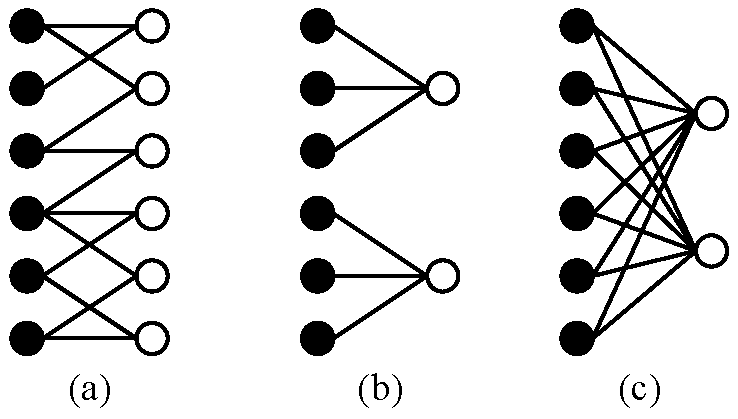
\includegraphics{figs-glossy/constraints.pdf}}
\vspace{-2ex}
\caption{Schematic representation of how records (solid circles) are organized into conflicts (empty circles) by different types of constraints: (a) A pair constraint, (b) A simple locus constraint, and (c) A complex locus constraint.} 
\label{fig:constraints:schematic}
\vspace{-2ex}
\end{figure}

A locus constraint binds together sets of records, where each set is informally the result of mapping the input records to a common identifier termed a locus. The set of loci can be thought of as a user-specified discretization of a space. For example, a density constraint is a locus constraint in which each locus corresponds to a unit area at a given scale. While a simple locus constraint uses a function that maps each record to exactly one locus, a complex locus constraint maps each record to a set of loci, i.e., the mapping function is a table function. The conflict structure of simple and complex locus constraints is illustrated in Figures~\ref{fig:constraints:schematic}(b) and~\ref{fig:constraints:schematic}(c).

By capturing in Glossy SQL multiple scales, record weighting, and constraint types that allow for natural specification of visual conflicts, we can concisely express the varied visualization use cases discussed in Section~\ref{sec:use:cases}.

\subsection{Examples: Solving the Use Cases}
\label{sec:use:cases:solved}

In this section, we show how to express the core use cases of Section~\ref{sec:use:cases} in Glossy SQL. While some use cases may seem different at first sight, a fair amount of commonality is exposed when they are expressed in Glossy SQL. For this reason, we omit detailed solutions when two use cases have substantially similar structure. 
We assume throughout this paper that input data is stored in a relational database system with appropriate indexing in place.  

\minisec{Rap artists selected by vocabulary size}
% About use case
We observe that Use Cases~\ref{ex:historical:events} and~\ref{ex:rappers} have essentially the same structure, and thus focus on presenting the Glossy SQL solution of Use Case~\ref{ex:rappers}.
To select rap artists for a zoomable line visualization based on vocabulary size, we employ a recursive Glossy SQL query, shown in Figure~\ref{fig:glossy:sql:rappers}. 

% Data details
The input table $rappers(\underline{id}, name, wordcount, pageviews)$ records information about each rap artist. While the meaning of the $id$ and $name$ columns is straightforward, the $wordcount$ column contains the number of distinct words used by an artist, obtained from an online lyrics database.\footnote{http://rap.genius.com} The $pageviews$ column contains the number of page views that the artist has received on the site; for this query, we use page views as a proxy for popularity.

% Query details
In the query, we use the \textbf{\texttt{RECURSE OVER}} construct to create a multi-scale global selection of rappers over five zoom levels. The construct implies that the output of a zoom level is used as input to the zoom level immediately lower. This ensures that data points will not disappear when zooming in, thus preserving zoom consistency. Each of the five scales are explicitly specified in the \textbf{\texttt{IN SEQUENCE}} clause. Each scale tuple has an integer $zoom$ column that can be used to select artists by scale later on, and an integer $bucketsize$ column that will control how rappers are grouped together into buckets.

While the outer \textbf{\texttt{WHERE}} clause specifies that we only select rappers with at least two songs, we further restrict the output by a locus constraint. In this constraint, we use the \textbf{\texttt{MAP BY}} clause to group rappers into buckets according to word count; rappers are mapped to buckets by arithmetic on the word count and bucketsize. For each bucket, we select at most 20 rappers and use \textbf{\texttt{SCALE LINEAR}} to maintain a linear density difference between dense and sparse buckets. As a final subtlety, we use a \textbf{\texttt{FILTER BY}} clause to ensure that our favorite band ``Digital Underground''  appears in the output, regardless of page views. Finally, we use the \textbf{\texttt{WEIGH BY}} clause to prioritize rappers based on their page views. 

% Query
\begin{figure}[!t]
\begin{center}
\begin{lstlisting}
SELECT id, name, wordcount, pageviews, zoom
FROM rappers ID id
   RECURSE OVER zoom, bucketsize 
   IN SEQUENCE 
   (5, 20), (4, 40), (3, 80), (2, 160), (1, 320)
WHERE songs > 1
WEIGH BY pageviews
SUBJECT TO
   FOREACH LOCUS
   MAP BY wordcount / bucketsize
   FILTER BY name <> 'Digital Underground'
   LIMIT 20 SCALE LINEAR
\end{lstlisting}
\vspace*{-2ex}
\caption{Selecting rappers on a line in Glossy SQL}
\label{fig:glossy:sql:rappers}
\end{center}
\vspace*{-5ex}
\end{figure}

\minisec{POI selected by star rating}
% About use case
To select points of interest (POI) for a zoomable map, our solution is another recursive Glossy SQL query, shown in Figure~\ref{fig:glossy:sql:poi}. However, in contrast to the previous example, a pair constraint is necessary to select POI with proper separation in 2-D. 
% Data details
In more detail, the input table $POI(\underline{id}, name, coord, stars)$ records the POI. The $coord$ column is a projected geographical coordinate, while the $stars$ column is a floating point value corresponding to the average star-rating given by reviewers.

% Query details
In the query, we use the \textbf{\texttt{RECURSE OVER}} syntax to create a multi-scale selection of POI over 19 zoom levels, which is a normal value for online maps. Again, the recursive selection guarantees that POI selected on lower zoom levels appear on all higher zoom levels. This time, we employ the \textbf{\texttt{IN RANGE}} clause to concisely specify the 19 integer values of the scales. Here, the $zoom$ column will be used both to enable selection of POI by scale later on, as well as to control the scale-dependent minimum proximity between POI that we will allow.

This time, we specify two constraints that restrict the selection, namely a locus constraint and a pair constraint. For the locus constraint, the \textbf{\texttt{MAP BY}} clause groups POI by map tile. This is achieved by the \texttt{TileCenter} function, which takes as input a point and a zoom level, and returns a label identifying the tile of the map in which the point is located at that zoom level. So in this example a locus corresponds to a tile. For each tile, we select at most 10 POI, and use \textbf{\texttt{SCALE LOG}} to maintain a logarithmic density difference between dense and sparse tiles. For the pair constraint, the \textbf{\texttt{WHERE}} clause specifies that two POI should not both be selected if they are in close proximity, measured in pixels in a scale-sensitive manner. Finally, we prioritize POI by their star-rating in the \textbf{\texttt{WEIGH BY}} clause. 

% Query
\begin{figure}[!t]
\begin{center}
\begin{lstlisting}
SELECT id, name, coord, stars, zoom
FROM poi ID id
   RECURSE OVER zoom 
   IN RANGE FROM 18 TO 0 
WEIGH BY stars
SUBJECT TO
   FOREACH LOCUS
   MAP BY TileCenter(coord, zoom)
   LIMIT 10 SCALE LOG
AND
   FOREACH PAIR x, y
   WHERE 
       DistancePixels(x.coord, y.coord, x.zoom) < 10
   DROP ONE
\end{lstlisting}
\vspace*{-2ex}
\caption{Selecting POI on a map in Glossy SQL}
\label{fig:glossy:sql:poi}
\end{center}
\vspace*{-5ex}
\end{figure}

\minisec{Placenames selected by relevance}
% About use case
To select placename labels for a zoomable map, we use an iterative Glossy SQL query, shown in Figure~\ref{fig:glossy:sql:placenames}. Since the query is iterative, the whole input is processed by the global selection at each zoom level, which allows labels to appear and disappear when zooming in. Additionally, we use a scale-dependent \textbf{\texttt{WHERE}} clause to remove labels that are irrelevant at a given scale.

% Data details
The input table $placenames(\underline{id}, label, polygon, importance)$ records the named places and their labels. The $label$ column records simply a text string, e.g., ``New York'' or ``Victoria''. The $polygon$ column is a geographical polygon that delineates the named place (e.g., continent, country or city). The $importance$ column records a user-defined weight for the label, e.g., a label for ``New York, NY'' is arguably more important than a label for ``White Plains, NY'', even though one is right next to the other.

% Query details
As stated above, we use the \textbf{\texttt{ITERATE OVER}} syntax in the query to allow placenames to be replaced by others when zooming in on the map. We combine this clause with the same \textbf{\texttt{IN RANGE}} clause that we use for the POI map. The query specifies a single locus constraint to ensure that we select at most $10$ labels per tile. Note that because the geometry of a named place is a polygon, this geometry may intersect many map tiles. So we use the \texttt{TileCenters} table function instead of the \texttt{TileCenter} function above so that we can map a given placename record to all the tiles that it intersects, again using tile labels as loci.  
Finallly, the \textbf{\texttt{WEIGH BY}} clause is used to rank labels according to their importance. 

% Query
\begin{figure}[!t]
\begin{center}
\begin{lstlisting}
SELECT id, label, polygon, importance, zoom
FROM placenames ID id
   ITERATE OVER zoom 
   IN RANGE FROM 18 TO 0
WHERE Area(polygon) / TileSize(zoom) 
      BETWEEN 0.1 AND 4
WEIGH BY importance
SUBJECT TO
   FOREACH LOCUS
   MAP BY TileCenters(polygon, zoom)
   LIMIT 10
\end{lstlisting}
\vspace*{-2ex}
\caption{Selecting placenames on a map in Glossy SQL}
\label{fig:glossy:sql:placenames}
\end{center}
\vspace*{-4ex}
\end{figure}

\begin{figure}[t]
\centering
\scalebox{0.40}{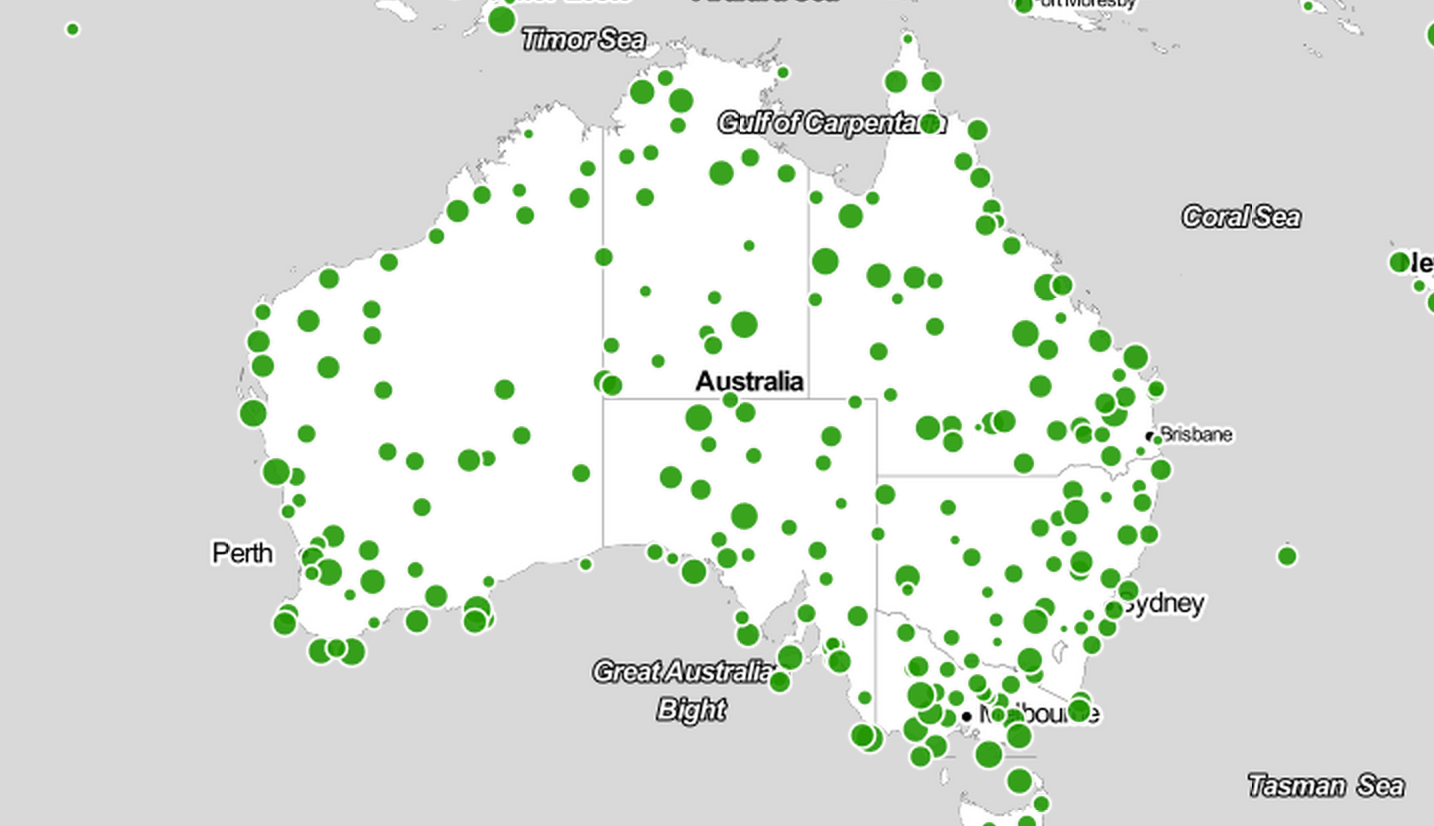
\includegraphics{figs-glossy/tourism_viz.png}}
\vspace{-1ex}
\caption{Combined visualization of POI and placenames.} 
\label{fig:tourism:viz}
\vspace{-2ex}
\end{figure}

\minisec{Additional Examples}
While the examples above illustrate the main features of Glossy SQL, they do not exhaust the whole gamut of possibilities. For example, consider that in most of the previous examples, one query was used to prepare all the necessary data for a given visualization. However, this does not need to be the case. Figure~\ref{fig:tourism:viz} shows a visualization that combines both POI and placenames in a single map. The visualization is constructed by taking the queries from the previous two examples and using the results of each as a layer in the visualization. 

Also, as discussed in Section~\ref{sec:use:cases}, not all visualizations are primarily structured around one or two dimensions. The use case of Example~\ref{ex:clusters} describes a multidimensional visualization using parallel coordinates. The data selection for that visualization can be accomplished in Glossy SQL by employing one locus constraint for each axis, limiting the number of lines crossing each unit area in a manner similar to what is done in Figure~\ref{fig:glossy:sql:rappers}. Weighing by distance to a cluster centroid can be expressed simply as a scalar subquery joining against a $centroids$ table. 

For brevity, we focus on the examples of Figures~\ref{fig:glossy:sql:rappers} to~\ref{fig:glossy:sql:placenames} when further evaluating our approach; however, they are representative of a much broader class of visualizations expressible in Glossy SQL.    

\subsection{Semantics}
\label{sec:semantics}
% Discussion:
% Semantics are to satisfy constraints, which includes the empty solution.
% Specifically, there may be several valid solutions to a Glossy query
% To make it more meaningful, we incorporate minimising loss of weight

% We are presenting Glossy as an extension of SQL. Important that 
% the semantics of e.g. SELECT, WHERE, FROM, etc remain the same as in SQL.

Armed with the intuitive understanding developed above, we formalize the semantics of Glossy SQL in this section. The semantics for a single scale is specified in terms of a global selection operator $\Sigma$ in Section~\ref{sec:semantics:global:selection}. Based on this specification, Section~\ref{sec:semantics:multiscale} defines the semantics of multi-scale global selection.

\subsubsection{Global Selection Operator}
\label{sec:semantics:global:selection}

We first focus on the semantics of single-scale Glossy SQL queries, i.e., queries that include neither an \textbf{\texttt{ITERATE OVER}} nor a \textbf{\texttt{RECURSE OVER}} clause. The main features of single-scale queries are then the specification of a set of constraints as well as of a weighting expression over the records of the input table. These specifications are holistically combined into a global selection of the records of the input table.

We abstract the weighting expression by a function $w: \mathbb{T} \; \rightarrow \; \mathbb{R}_{0}^+$, where $w$ maps a tuple from the domain of all possible tuples $\mathbb{T}$ to a nonnegative real value.\footnote{The domain of all possible tuples in a relation $\mathbb{T}$ can be defined in the usual way by the cartesian product of the domains of the corresponding relation schema's attributes~\cite{RG02:CowBook}.} To model how constraints influence global selection, we must introduce the notion of a conflict. 

\begin{definition}[Conflict]
A conflict is a 2-tuple $c = (k, R)$, where $k \; \in \; \mathbb{N}$ is the maximum number of records that are allowed to survive after the global selection from the conflict $c$, and $R$ is a set of records from the input table with $|R| > k$. \mathendbox
\end{definition}
 
A conflict thus captures a set of records out of which only $k$ may be presented in the visualization. As we have seen in Section~\ref{sec:use:cases:solved}, these conflicts are typically associated with visual restrictions such as information density. 
 
A constraint $K$, when applied to an input relation $I$, specifies a set of conflicts $C$. The precise set of conflicts $C$ is defined according to the whether the constraint is a pair or a locus constraint. 

\begin{definition}[Conflict set for pair constraint]
A pair constraint $K$ defines a set of conflicts $C = \{ (k_1, R_1), (k_2, R_2), \ldots, (k_n, R_n) \}$ over an input relation $I$, where:
\begin{enumerate}[label=(\alph*)]
\item all $k_i = 1$ if the constraint's \textbf{\texttt{DROP}} clause specifies \textbf{\texttt{ONE}}, or all $k_i = 0$ if the \textbf{\texttt{DROP}} clause specifies \textbf{\texttt{BOTH}};
\item the $R_i$ contain exactly a pair of records each, corresponding to the records from the input relation paired by the join $I \bowtie_{Cnd} I$, where $Cnd$ is the condition specified in the constraint's \textbf{\texttt{WHERE}} clause. \mathendbox
\end{enumerate}   
\label{def:conflict:set:pair}
\end{definition} 

\begin{definition}[Conflict set for locus constraint]
A locus constraint $K$ defines a set of conflicts $C = \{ (k_1, R_1), (k_2, R_2), \ldots, (k_n, R_n) \}$ over an input relation $I$, where:
\begin{enumerate}[label=(\alph*)]
\item each $(k_i, R_i)$ corresponds to the conflict in exactly one locus $l_i$;
\item the possible loci $l_i$ are given by a set of labels $\mathbb{L}$, and the mapping of records to loci is given by a non-injective, non-surjective mapping function $f: \mathbb{T} \rightarrow \mathcal P (\mathbb{L})$ specified in the constraint's \textbf{\texttt{MAP}} clause, where $\mathcal P (\mathbb{L})$ is the power set of $\mathbb{L}$;
\item each record must be mapped to at least one locus;
\item when a record is mapped to multiple loci, it appears in the $R_i$ of the conflicts corresponding to each of these loci, when no \textbf{\texttt{FILTER BY}} clause is given;
\item when a \textbf{\texttt{FILTER BY}} clause is given, it is further ensured that none of the records in $R_i$ violate the condition $Cnd$ specified in the constraint's \textbf{\texttt{FILTER BY}} clause;
\item the values of $k_i$ are given by evaluation of the integer expression in the constraint's \textbf{\texttt{LIMIT}} clause, when no \textbf{\texttt{SCALE}} clause is given;
\item when a \textbf{\texttt{SCALE}} clause is given, the values of $k_i$ are scaled either linearly or a logarithmically as a fraction of the maximum value of all $k_i$ as defined above without scaling. 
\mathendbox 
\end{enumerate}
\label{def:conflict:set:locus}
\end{definition} 
 
Assume a Glossy SQL query is composed of constraints $\langle K_1, K_2, \ldots, K_m\rangle$, with associated sets of conflicts $\langle C_1, C_2, \ldots, C_m\rangle$ over the input. We define the conflict set of the query to be $\mathbb{C} = C_1 \;\cup\; C_2 \;\cup\; \ldots \; C_m$. Given a conflict set $\mathbb{C}$ over an input relation $I$, and a weighting function $w$, we can define the global selection operator as:
 
 \begin{definition}[Global Selection Operator]
The~global selection operator $\Sigma_{\mathbb{C}}^{w}: \mathbb{I} \rightarrow \mathbb{I}$, where $\mathbb{I}$ is the power set of $\mathbb{T}$, maps an input relation instance $I \; \in \; \mathbb{I}$ to an output relation instance $O \subseteq I$ s.t.:
\begin{enumerate}[label=(\alph*)]
\item $O$~contains at most $k_{i}$ surviving records for each of the conflicts $c_{i} = (k_{i},R_{i}) \; \in \; \mathbb{C}$;
\item the sum of the record weights in $O$ is maximal wrt.~all such qualifying relation instances.  \mathendbox 
\end{enumerate}
 \end{definition} 

Our notions of a visual conflicts as well as of finding a maximal-weight solution that resolves all conflicts are similar to the ones introduced by Kefaloukos et al.~\cite{KefaloukosSZ14:CVL}. It is easy to see that their conclusion that finding such a solution is equivalent to the set multi-cover problem also applies to the global selection operator. Since this problem is NP-hard, we relax the semantics of global selection to allow for the use of heuristics or approximate algorithms to compute global selection solutions. In contrast to~\cite{KefaloukosSZ14:CVL}, however, our definitions above constitute a general framework that transcends the visualization of geographical maps.     

To complete the description of the semantics of single-scale Glossy SQL queries, we observe that the \textbf{\texttt{SELECT}} clause is equivalent to a projection over the input table. So a single-scale Glossy SQL query over input relation $I$, with weighting function $w$, constraints $\langle K_1, K_2, \ldots, K_m\rangle$ yielding an associated set of conflicts $\mathbb{C}$, a \textbf{\texttt{WHERE}} clause with condition $Cnd$, and projecting attributes $\langle a_1, a_2, \ldots, a_l \rangle$ corresponds to the expression $\pi_{\langle a_1, a_2, \ldots, a_l \rangle} (\Sigma_{\mathbb{C}}^{w}(\sigma_{Cnd}(I)))$ in the extended relational algebra with the global selection operator. 
 
\subsubsection{Multi-Scale Global Selection}
\label{sec:semantics:multiscale}

We now turn to the semantics of multi-scale Glossy SQL queries. These queries include either an \textbf{\texttt{ITERATE OVER}} or a \textbf{\texttt{RECURSE OVER}} clause, which specify a sequence $S$ of tuples with the same schema s.t.~each tuple encodes information about a given scale. Multi-scale Glossy SQL queries apply a global selection at each scale, but construct the input for each scale differently according to whether they are iterative or recursive.

\begin{algorithm}
\caption{Conceptual Evaluation of Multi-Scale Glossy SQL.}
\begin{algorithmic}
\STATE $R \leftarrow I$
\STATE $O \leftarrow \emptyset$
\FOR{Tuple $t$ in $S$}  
\STATE $L_I \leftarrow \sigma_{Cnd}(t \times R)$
\STATE Derive set of conflicts $\mathbb{C}$ from $\langle K_1, K_2, \ldots, K_m\rangle$ and $L_I$
\STATE $L_O \leftarrow \Sigma_{\mathbb{C}}^{w}(L_I)$ 
\IF{\textbf{\texttt{RECURSE OVER}} $S$}
\STATE $R \leftarrow \pi_{\langle i_1, i_2, \ldots, i_p \rangle} L_O$ 
\ENDIF
\STATE $O \leftarrow O \; \cup \; L_O$
\ENDFOR
\RETURN $\pi_{\langle a_1, a_2, \ldots, a_l \rangle} (O)$
\end{algorithmic}
\label{alg:conceptual:multiscale}
\end{algorithm}

The semantics of multi-scale Glossy SQL queries can be specified by a conceptual evaluation program, as shown in Algorithm~\ref{alg:conceptual:multiscale}. Similarly to the single-scale case, we assume a query over input relation $I$ with attributes $\langle i_1, i_2, \ldots, i_p \rangle$, with weighting function $w$, constraints $\langle K_1, K_2, \ldots, K_m\rangle$, a \textbf{\texttt{WHERE}} clause with condition $Cnd$, and projecting attributes $\langle a_1, a_2, \ldots, a_l \rangle$.   


The algorithm iterates over the sequence $S$ one tuple at a time. Each tuple is cross-joined with the the current input tuples in $R$. In the case of an iterative multi-scale Glossy SQL query, these input tuples always correspond to the entire input relation $I$; in the case of a recursive multi-scale Glossy SQL query, however, the input tuples in $R$ correspond to the surviving tuples from the global selection of the previous scale. The algorithm derives the conflict set $\mathbb{C}$ from the constraints in the query in a way that is sensitive to the current input and scale. This process consists of producing conflict sets consistent with Definitions~\ref{def:conflict:set:pair} and~\ref{def:conflict:set:locus} from the previous subsection, but considering $L_I$ as the input relation. The output for the current scale $L_O$ is the result of the global selection over $L_I$ with conflict set $\mathbb{C}$ and weighting function $w$. This partial output is collected into a global output relation, which is projected according to the query before the final result is produced.  

\section{Pure SQL Translation}
\label{sec:sql:translation}

In this section, we present the translation of the Glossy SQL syntax introduced in Section~\ref{sec:syntax} to SQL. Without loss of generality, we conform to the SQL dialect and function library offered by PostgreSQL\footnote{http://www.postgresql.org/}, as used in the implementation of Glossy. Extension to other relational DBMS is conceptually straightforward.  

We start by discussing the translation of single-scale global selections in Section~\ref{sec:translation:global:selection}. Based on this translation, we present how to express in SQL multi-scale global selections in Section~\ref{sec:translation:multiscale}.  

\subsection{Global Selection Operator}
\label{sec:translation:global:selection}

We first discuss how to compute in SQL the elements that should be kept at a single scale. As discussed in Section~\ref{sec:semantics}, the global selection operator $\Sigma_{\mathbb{C}}^{w}$ specifies this single-scale computation, encoding the resolution of a set of visual conflicts $\mathbb{C}$ weighed by a weighting function $w$. The weighting function $w$ is directly specified in the Glossy SQL extended syntax through the \textbf{\texttt{WEIGH BY}} clause. The set of conflicts $\mathbb{C}$, on the other hand, must be derived from the constraints specified in the \textbf{\texttt{SUBJECT BY}} clause. Once $\mathbb{C}$ is derived, it is necessary to resolve all conflicts automatically by picking records to be deleted through an appropriate algorithm.  

Section~\ref{sec:calc:conflicts} examines how to compute $\mathbb{C}$ from the constraints, while Section~\ref{sec:resolve:conflicts} reviews algorithmic approaches to globally resolving conflicts. 

\subsubsection{Calculating the Set of Conflicts $\mathbb{C}$}
\label{sec:calc:conflicts}

We examine below how to translate both pair as well as locus constraints to SQL statements that derive conflict sets. To do so, some notation is required. The translation of Glossy SQL fragments is denoted by $\denote{$\cdot$}_E$, where $E$ is an environment. An environment is a set containing mappings of variable names given in a constraint to appropriate table aliases in the generated SQL. For simplicity, we omit specification of the environment in contexts where variable mappings are not required.  

The input to conflict calculation is the input table, potentially augmented with fields from the scale column list (see syntax in Figure~\ref{fig:glossy:sql:syntax}). Below, we assume that the scale to which the global selection is currently being applied be determined by an \texttt{iteration} column added to the augmented input table \texttt{current\_input}. Details on the augmentation process are given in Section~\ref{sec:translation:multiscale}. 

\minisec{Pair Constraints}
We start by examining pair constraints. Every conflict specified by a pair constraint involves two records from the input table, identified by the key given in the schema or explicitly in the \textbf{\texttt{ID BY}} clause (in case a key is not given, our translator generates a surrogate automatically). We assume for simplicity that the key is given by a column \texttt{K} of \texttt{current\_input}. Likewise, we assume that the weight is calculated into a column \texttt{weight}.  

Intuitively, generating pairs is a self-join operation on the \texttt{current\_input} table, and each pair represents a conflict that can be resolved by letting either one record survive or none.~This intuition is captured by the translation below: \\

\denote{\lstinline!FOREACH PAIR!$\;x,\;y\;$\lstinline!WHERE!$\;C\;$\lstinline!DROP ONE!} =
\begin{lstlisting}[mathescape,escapechar=!]
   SELECT
     -- conflict identifier is {cid, iteration}
     -- climit states max survivors
     l.K || '_' || r.K AS cid,
     l.iteration AS iteration,
     1 AS climit,
     -- record information
     Unnest(array[l.K, r.K]) AS rid,
     Unnest(array[l.weight, r.weight]) AS weight
   FROM current_input l JOIN current_input r
   ON   l.K < r.K AND
        l.iteration = r.iteration AND
        !\denote{$C$}$_{\{x \rightarrow l,\;y \rightarrow r \}}$!
\end{lstlisting}

The SQL statement returns sets of conflicts containing two records each, generated as expected by a self-join, and stating in the \texttt{climit} attribute that a single surviving record will resolve the conflict. The \texttt{Unnest} function creates one output record for each element in the given array. The translation of the \textbf{\texttt{WHERE}} clause must include the appropriate translation of the condition supplied by the user, taking into account the variable names $x$ and $y$. Note that omitting the \textbf{\texttt{WHERE}} clause above is equivalent to specifying the condition \textbf{\texttt{true}}, while specifying the clause \textbf{\texttt{DROP BOTH}} would yield instead a value of zero for the \texttt{climit} column returned by the SQL statement.
 
\minisec{Locus Constraints}
We now consider locus constraints. In a locus constraint, records are filtered by a constraint-specific \textbf{\texttt{FILTER BY}} clause, if one is provided. Then, a non-injective non-surjective function $f$ of records to sets of loci is applied, i.e., the application of $f$ results in each record being mapped to a set of loci, and thus each locus can potentially contain one or more records. Since conflicts are defined as loci with excessive numbers of records, resolving conflicts consists of reducing the number of records in each locus to at most the number $k$ given in the \textbf{\texttt{LIMIT}} clause. \\

\denote{\lstinline!FOREACH LOCUS MAP BY!$\;f(x)\;$\lstinline!  FILTER BY!$\;C\;$\lstinline!LIMIT !$\;k$} =
\begin{lstlisting}[mathescape,escapechar=!]
   SELECT
    !\denote{$f(x)$}$_{\{x \rightarrow c\}}$! AS cid,
    iteration AS iteration,
    !\denote{$k$}! AS climit,
    Unnest(array_agg(K)) AS rid,
    Unnest(array_agg(weight)) AS weight
   FROM current_input c
   WHERE !\denote{$C$}$_{\{x \rightarrow c\}}$!
   GROUP BY !\denote{$f(x)$}$_{\{x \rightarrow c\}}$!, iteration
   HAVING count(*) > !\denote{$k$}!
\end{lstlisting} 
 
The SQL statement applies the function $f$ to obtain one or many loci, depending on whether $f$ is defined as a simple function or as a table function. Each of the locus labels returned by $f$ serves both as a conflict identifier and as a grouping value. Similarly to the translation of a pair constraint, the SQL statement employs \texttt{Unnest} to expand the multiple input records mapped to the same conflict identifier into a corresponding number of output records, and the \texttt{iteration} column to separate conflicts in different scales. In addition, in the translations of the application of $f$ and of the condition $C$, we assume the variable $x$ is the alias specified for the input table in the query, which needs to be mapped accordingly. In the case of a multi-scale query with a separate alias for the sequence of scales, the environment mapping simply needs to be extended by this additional alias. 

\minisec{\texttt{SCALE} Clause}
Recall from Figure~\ref{fig:glossy:sql:syntax} that an optional \textbf{\texttt{SCALE}} clause may be specified for a locus constraint. Since the number $k$ given in the \textbf{\texttt{LIMIT}} clause is a hard bound, it is often the case that some loci will require that far more records be eliminated to resolve conflicts than others. For example, with a limit of 16 records per locus, loci with 20 records and 40 records will lead to deletion of 4 and 24 records respectively. This asymmetry may destroy distributional properties that some visualizations require to be maintained. In order to deal with this issue, the \textbf{\texttt{SCALE}} clause specifies that the limit bound should be scaled dynamically according to the maximum number of records in any given locus. The adjustment may follow either a linear or a logarithmic function.  

Specification of a \textbf{\texttt{SCALE}} clause affects the SQL translation above by replacing \denote{$k$} in the \texttt{climit} attribute with an appropriate expression involving a scalar subquery. In the case of \textbf{\texttt{LINEAR}} scaling, the resulting expression is:

\begin{lstlisting}[mathescape,escapechar=!]
  ceil(!\denote{$k$}!*(count(*)::float / 
             (SELECT max(cnt)
              FROM 
               (SELECT iteration, count(*) AS cnt 
                FROM current_input c1
                WHERE !\denote{$C$}$_{\{x \rightarrow c1\}}$!
                GROUP BY !\denote{$f(x)$}$_{\{x \rightarrow c1\}}$!,iteration) m              
              WHERE m.iteration = c.iteration)           
\end{lstlisting} 

%\kostas{Rewrote above SQL to shorter and equivalent query (I think). Need to verify.}

The scalar query scales the number of allowed survivors in each locus by the fraction of the number of records in the locus over the maximum number of records in any locus, within the same iteration. As can be seen from the query above, a simple and intuitive feature for a declarative language for visualizations can lead to a substantially complex underlying translation. The translation for logarithmic scaling is similar, but takes $\max(1,\log(y))$ for $y$ in both numerator and denominator of the fraction above. 

\minisec{From Constraints to $\mathbb{C}$}
The complete set of visual conflicts $\mathbb{C}$ is given by evaluating the union of the conflict sets for each constraint. Assume that a set $\{K_1, K_2, \ldots, K_m\}$ of constraints $K_i$ is specified in a Glossy SQL statement. Let $Q_\mathbb{C}$ be the query that calculates $\mathbb{C}$ for these constraints. Then:

\begin{lstlisting}[escapechar=\!]  
   !$Q_\mathbb{C}$ = !!\denote{$K_1$}! UNION ALL !\denote{$K_2$}! UNION ALL !$\ldots$! !\denote{$K_m$}! 
\end{lstlisting} 

\subsubsection{Resolving Conflicts}
\label{sec:resolve:conflicts}  

As pointed out in Section~\ref{sec:semantics}, conflict resolution can be modeled as finding a solution to a set multi-cover formulation~\cite{KefaloukosSZ14:CVL}. Kefaloukos et al.~have shown that a simple heuristic is effective: Sort the records in each conflict $c$ by weight, and pick the $k_c$ survivors with largest weight in each set. For completeness, we re-state in the following the SQL formulation of this heuristic, adapting it to our translation procedure.

As above, let $Q_\mathbb{C}$ be the query that determines $\mathbb{C}$ for the set of constraints given in a Glossy SQL statement. Then, for each scale, we determine the survivor records by: 

\begin{lstlisting}[escapechar=!]
SELECT *
FROM current_input c
WHERE NOT EXISTS (
  SELECT 'x'
  FROM (
   SELECT rid, iteration
   FROM (SELECT rid,
                iteration, 
                ROW_NUMBER() OVER (
                   PARTITION BY cid, iteration 
                   ORDER BY weight DESC) 
                   AS row_number, 
                climit
         FROM (!$Q_\mathbb{C}$!) conflicts) solution
   WHERE solution.row_number >
                      solution.climit) deleted
  WHERE 
    c.K = deleted.rid AND
    c.iteration = deleted.iteration)
\end{lstlisting}

Note that in the SQL statement, if many records have the same value for cutoff weight, the selection of surviving records within the cutoff is arbitrary. It is possible to envision incorporating randomization in this process. If all records were weighted equally, this strategy would then simulate a random sampling process as a special case. 

\subsection{Multi-Scale Global Selection}
\label{sec:translation:multiscale}

Building on the ground translation of single-scale global selection, we now present the translation of multi-scale Glossy SQL statements. The distinctive feature of these statements is the specification of either an \textbf{\texttt{ITERATE OVER}} or a \textbf{\texttt{RECURSE OVER}} clause, which are analyzed separately in Sections~\ref{sec:translation:iterative} and~\ref{sec:translation:recursive}.   

\subsubsection{ITERATE OVER Construct}
\label{sec:translation:iterative}

The translation in Section~\ref{sec:translation:global:selection} relied on the existence of a \texttt{current\_input} table, which consists of an augmented input table according to scale. In particular, one of the columns expected in \texttt{current\_input} -- the \texttt{iteration} column -- is an explicit representation of the scale being considered. The translation of a Glossy SQL statement including an \textbf{\texttt{ITERATE OVER}} clause is elegantly achieved by an appropriate definition of the \texttt{current\_input} table.

Recall from Section~\ref{sec:semantics} that an iterative global selection consists of the union of global selections of the input table matched against each record of an ordered table representing scales. The scales table can be defined either by a \textbf{\texttt{RANGE}}, \textbf{\texttt{SEQUENCE}}, or subquery. It is straightforward to translate these constructs into SQL, so we assume the existence of a \texttt{scales} table. The \texttt{scales} table includes an \texttt{iteration} column, generated by computing a row number across all records. Furthermore, we assume the input table given by the user is simply called \texttt{input}. Then,

\begin{lstlisting}[escapechar=!]
  !\texttt{current\_input} = !
   SELECT *, !\denote{$w$}! AS weight
   FROM input, scales
   WHERE !\denote{$C$}!   
\end{lstlisting}

In the SQL statement above, $w$ represents the weighting expression given in the \textbf{\texttt{WEIGH BY}} clause, and $C$ the condition given in the top-level \textbf{\texttt{WHERE}} clause. For simplicity, we assume there are no naming conflicts with the columns in the schemas of \texttt{input} and \texttt{scales}, and that the input table already contains an identifying column \texttt{K}. 

Plugging the definition of \texttt{current\_input} above into the translation of Section~\ref{sec:resolve:conflicts} completes the translation of an iterative, multi-scale Glossy SQL statement. 

\subsubsection{RECURSE OVER Construct}
\label{sec:translation:recursive}

Assuming again the existence of tables \texttt{input} and \texttt{scales}, we turn our attention to the translation of recursive Glossy SQL statements. In contrast to iterative Glossy SQL, recursive Glossy SQL must consider the output of global selection of scale $s$ as the input to scale $s+1$. To achieve this effect, we translate recursive Glossy SQL to a recursive SQL query.

The overall structure of this recursive SQL query is given by:

\begin{lstlisting}[escapechar=!]
   WITH RECURSIVE multiscale_select AS (
    !$Q_B$! UNION ALL !$Q_R$!)
   SELECT !\denote{\{expression\_list\}}! 
   FROM multiscale_select;
\end{lstlisting}  

In the recursive SQL statement, $Q_B$ is the query for the base case, while $Q_R$ is the query for the recursive term. The \texttt{\{expression-list\}} is given by the topmost \textbf{\texttt{SELECT}} clause in the Glossy SQL statement (see Figure~\ref{fig:glossy:sql:syntax}).    

Both $Q_B$ and $Q_R$ are very similar in structure to the single-level translation of Section~\ref{sec:resolve:conflicts}; however, these queries must consider carefully constructed \texttt{current\_input} tables. For $Q_B$, the current input should consider the input table joined with the tuple corresponding to the first scale:

\begin{lstlisting}[escapechar=!]
  !$Q_B$: \texttt{current\_input} = !
   SELECT *, !\denote{$w$}! AS weight
   FROM input, scales
   WHERE scales.iteration = 1 AND !\denote{$C$}!   
\end{lstlisting}

Note the similarity between this formulation for \texttt{current\_input} with the one from Section~\ref{sec:translation:iterative}. Likewise, $Q_B$ is obtained by plugging this definition of \texttt{current\_input} into the translation of Section~\ref{sec:resolve:conflicts}. 
    
 The formulation of \texttt{current\_input} for $Q_R$ is more sophisticated. We could in principle simply join the tuples currently in the recursive self-reference for \texttt{multiscale\_select} with the next tuple in the \texttt{scales} table. However, this simple strategy would preclude us from using any index structures present over the \texttt{input} table to compute the global selections of any of the recursive levels. Instead, we join back with the \texttt{input} table matching the appropriate record identifiers from the recursive self-reference, enabling query rewrites of the DBMS to take advantage of the \texttt{input} table's physical structures directly:
 
\begin{lstlisting}[escapechar=!]
  !$Q_R$: \texttt{current\_input} = !
   SELECT *, !\denote{$w$}! AS weight
   FROM input
   JOIN (
     SELECT multiscale_select.K, scales.*
     FROM multiscale_select, scales
     WHERE scales.iteration =
            multiscale_select.iteration + 1
        ) scale_rids
   USING (K)
   WHERE !\denote{$C$}! 
\end{lstlisting}
 
In the SQL statement, note that we must evaluate $C$ at each level, since it may reference the scale tuple. If only references to the input table are present in $C$, then the evaluation of the condition on the recursive case can be optimized away.  

To obtain $Q_R$, all that is left is to plug  this definition of \texttt{current\_input} into the translation of Section~\ref{sec:resolve:conflicts}. This last step completes the translation of Glossy SQL.

\section{Experimental Evaluation}
\label{sec:experimental:evaluation}

In this section, we evaluate the performance of Glossy SQL queries when compiled to pure SQL by the  translation of Section~\ref{sec:sql:translation} and run over an existing RDBMS (PostgreSQL). The goals of our evaluation are to show that: 
%In the experimental evaluation of Glossy, we will show that: 
(1)~The Glossy SQL compiler produces efficient and scalable SQL target queries for a range of Glossy SQL constructs; (2)~Glossy SQL can be used to efficiently compute the main use cases presented in Sections~\ref{sec:use:cases} and detailed in Section~\ref{sec:use:cases:solved}; and (3)~The performance of Glossy is either competitive or superior to the performance of a recent SQL compilation approach specialized to the domain of geographical maps. 

%and related system called CVL.

\subsection{Setup}
% measurements are of generated code, i.e. SQL running in DB:
\minisec{Software and Hardware Configuration}
We have evaluated Glossy by executing the SQL output of the Glossy SQL compiler in an existing RDBMS. The database used for evaluation was PostgreSQL 9.3.5 with PostGIS extensions. The RDBMS was configured with 2GB cache, 2GB work memory and 1 GB shared buffers. The database ran on hardware with a 2 GHz Intel Core i7 processor having 4 cores, 256 KB L2 cache, 6 MB L3 cache, 16 GB of RAM, and an Apple SSD SM0256F with 251 GB. The Glossy SQL compiler, which was implemented in Python, is not in the critical path of this experimental evaluation.

\minisec{Comparison with CVL}
We have chosen to compare Glossy to the recent approach of Kefaloukos et al.~\cite{KefaloukosSZ14:CVL}, who propose a domain-specific language for generalization of multi-scale geographical maps called CVL. The same algorithmic approach to conflict resolution is used in CVL and in Glossy, namely the sort-based heuristic explained in Section~\ref{sec:resolve:conflicts}. This is helpful because our evaluation then reflects the contrasting quality of the SQL code generated by Glossy as per the translation of Section~\ref{sec:sql:translation} when compared to the SQL code generated by the publicly-available CVL compiler.\footnote{https://github.com/dmslab/declarativecartography} Obviously, since CVL is restricted to geographical maps, we only compare the two systems within that domain, and refrain from comparison in use cases that are only expressible in Glossy SQL.  

\begin{table}[ht]
\vspace{-1ex}
\begin{center}
\tabcolsep=0.15cm
\begin{tabular}{|l|l|l|l|}
\hline
\multirow{3}{*}{\textbf{Dataset}} & \multirow{2}{*}{\textbf{Data}}      & \multirow{2}{*}{\textbf{Dimension}} & \textbf{Input}    \\
                                                        & \multirow{2}{*}{\textbf{Source}}  & \multirow{2}{*}{\textbf{and Type}}    & \textbf{Size}     \\
                                                        &                             &                                    & \textbf{(rows)}  \\
\hline
Rap Lyrics & Genius & 1-D word counts & 13K \\
Airports & OpenFlights & 2-D points & 7K \\
Points of Interest & OpenStreetMap & 2-D points & 520K \\
Placenames & GeoNames & 2-D points & 10K \\
Synthetic Places & Synthetic & 2-D polygons & 1M \\
\hline
\end{tabular}
\vspace{-1ex}
\caption{Datasets used in experiments}
\label{tab:glossy:datasets}
\end{center}
\vspace{-3ex}
\end{table}%

\minisec{Datasets}
The data used to evaluate Glossy consists of real, publicly-available datasets from OpenFlights,\footnote{http://openflights.org/data.html} GeoNames,\footnote{http://www.geonames.org/export/} OpenStreetMap\footnote{http://planet.openstreetmap.org/} and Genius,\footnote{http://rap.genius.com/} as well as a synthetic dataset. The datasets correspond to the use cases described in Section~\ref{sec:use:cases} and solved in detail in Section~\ref{sec:use:cases:solved}. The characteristics of these datasets are summarized in Table~\ref{tab:glossy:datasets}. We augmented the tourism dataset from OpenStreetMap with synthetic star ratings in the range $\lbrack 1, 5 \rbrack$, normally distributed around the value $3$ and with a standard deviation of $1$.  We further created a synthetic dataset with one million named places corresponding to continents, countries, regions, cities and neighborhoods. The goal of this dataset was to stress the use of more sophisticated geometric features in the underlying database with a relatively large dataset for visualization. To achieve this goal, we associated to each synthetic named place a rectangular geometry centered at a point with both latitude and longitude generated uniformly at random. The units for latitude, longitude, and side lengths were taken from a spherical mercator projection as commonly used by mapping services such as OpenStreetMap. To create geometries of varying sizes, squares were first generated with half-side lengths drawn from a normal distribution around the value $100$ and with a standard deviation of $10^7$. To avoid either negative or too small side lengths, we have taken absolute values for half-side lengths and forced them to $100$ whenever they were smaller than that value. We then cropped geometries at the boundaries of the projection so that they would be fully contained within the world map. For the geographical visualizations throughout this paper, we have used background maps from Stamen.\footnote{http://maps.stamen.com/}

\minisec{Queries}
The Glossy SQL queries used in our evaluation are variants of the queries presented in Section~\ref{sec:use:cases:solved} and Figures~\ref{fig:glossy:sql:rappers} to~\ref{fig:glossy:sql:placenames}. Throughout our measurements, we have observed only negligible differences in the running times of a given query under the same configuration. So we report below the median of three runs for each measurement. We provide further details on procedures for varying query formulations and scaling data in the relevant experiment descriptions below.  

\begin{figure}[!t]
\centering
\scalebox{0.45}{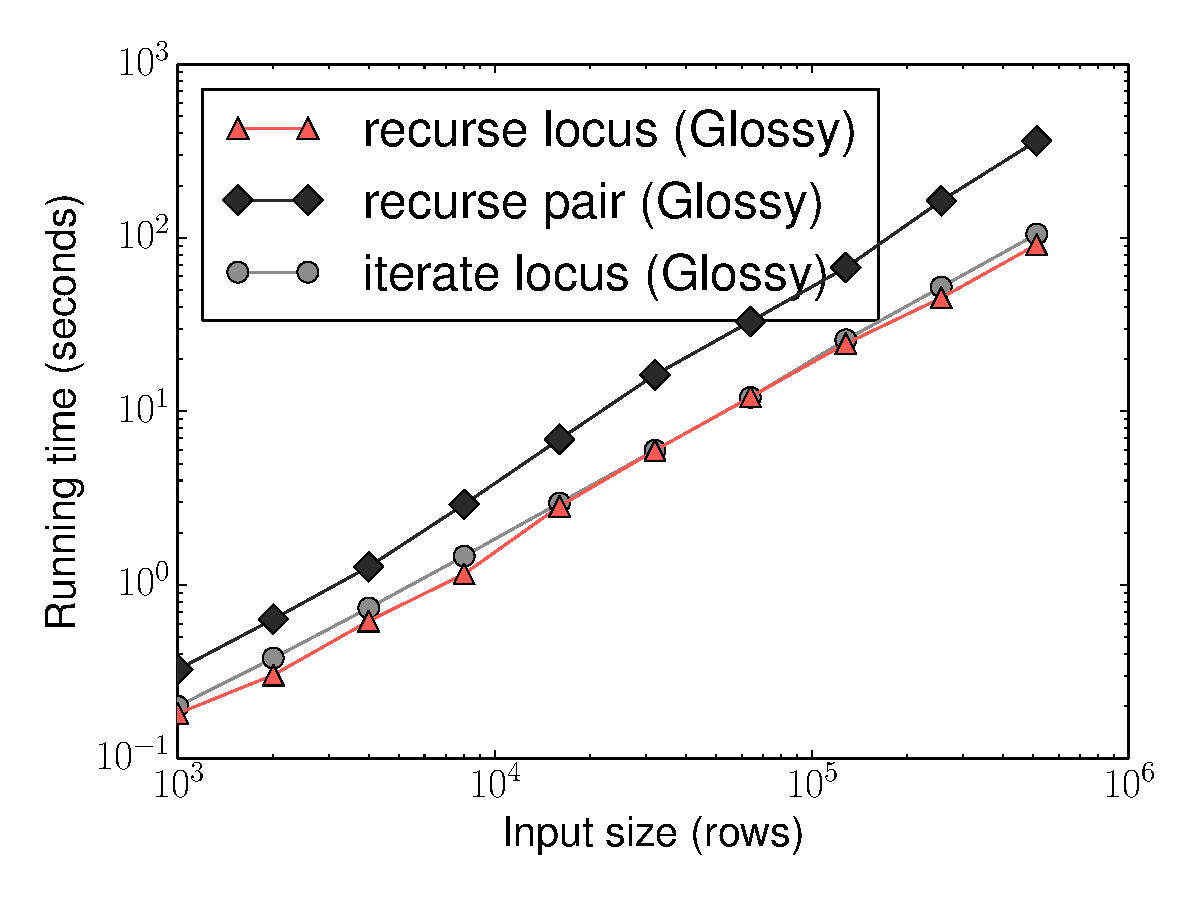
\includegraphics{figs-glossy/scalability.pdf}}
\vspace{-4ex}
\caption{Scalability of three Glossy query-types on POI data: (triangles) recursive query with locus constraint, (diamonds) recursive query with pair constraint, (circles) iterative query with locus constraint.}
\vspace{-3ex}
\label{fig:glossy:scalability}
\end{figure}


\begin{figure*}[!t]
     \begin{minipage}{0.32\linewidth}
        \centerline{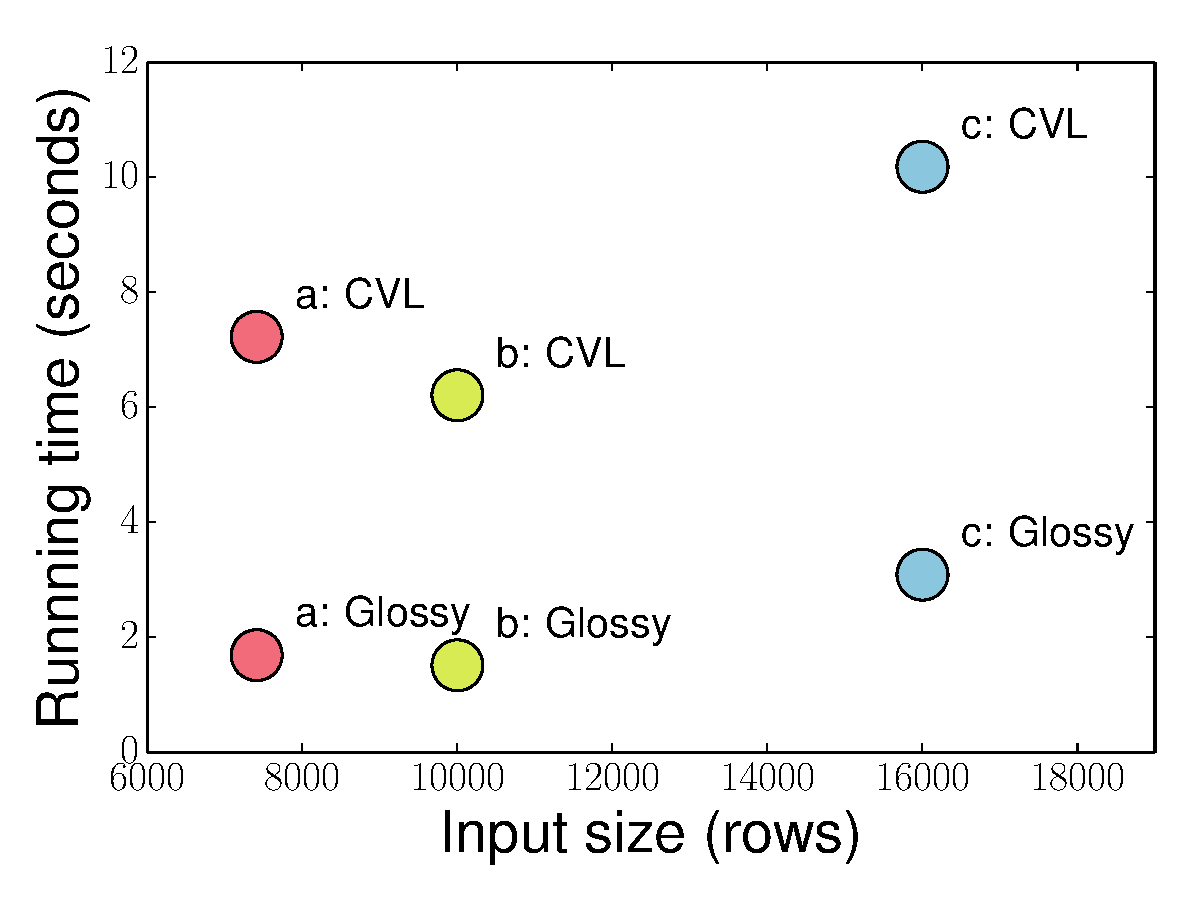
\includegraphics[width=1\linewidth]{figs-glossy/comparison_glossy_vs_cvl_locus.pdf}}
        \vspace{-3ex}
        \caption{Response time of equivalent queries in Glossy vs. CVL with locus constraint: (a) Airports, (b) Placenames, (c) Points of Interest.}\label{fig:glossy:vs:cvl:locus}
    \end{minipage} \hfill
    \begin{minipage}{0.32\linewidth}
        \centerline{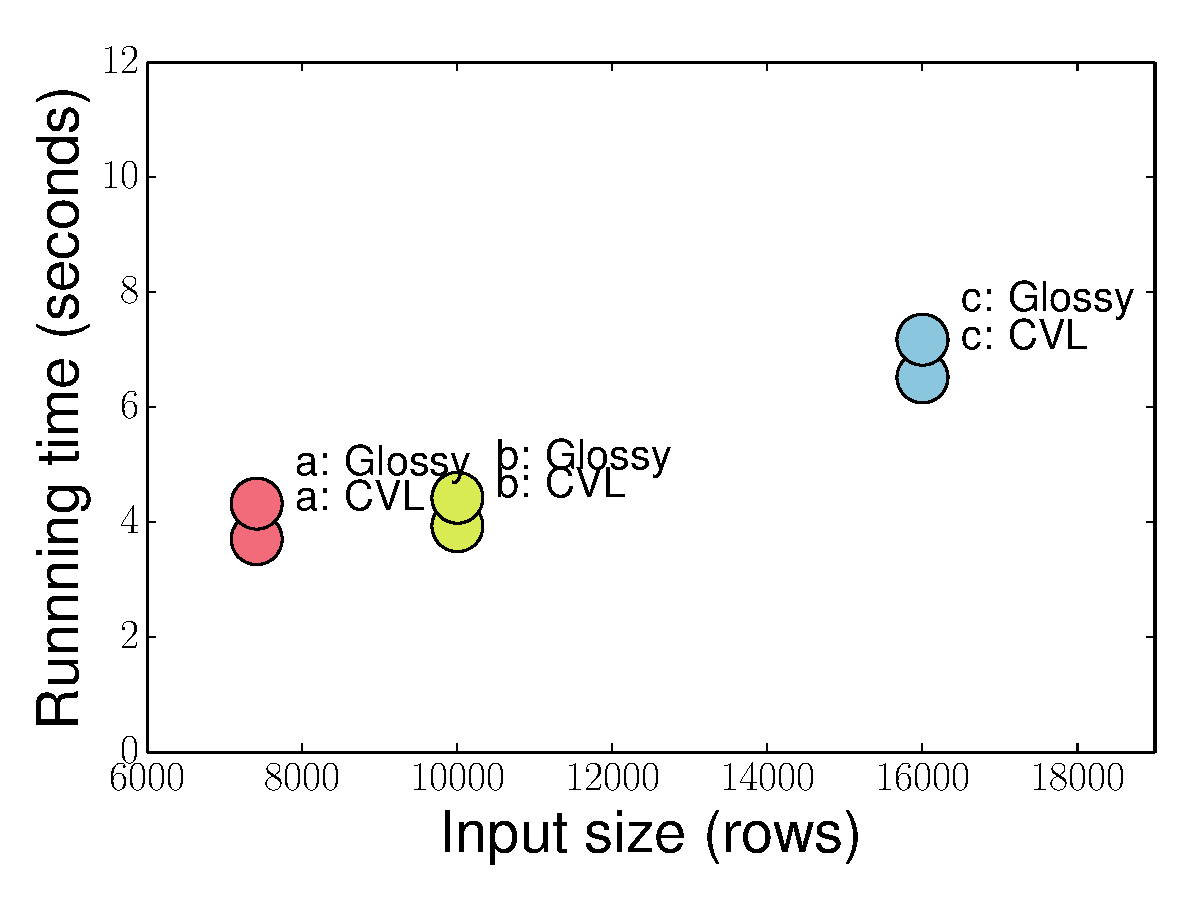
\includegraphics[width=1\linewidth]{figs-glossy/comparison_glossy_vs_cvl_pair.pdf}}
        \vspace{-3ex}
        \caption{Response time of equivalent queries in Glossy vs. CVL with pair constraint: (a) Airports, (b) Placenames, (c) Points of Interest.} \label{fig:glossy:vs:cvl:pair}
    \end{minipage} \hfill
        \begin{minipage}{0.32\linewidth}
        \centerline{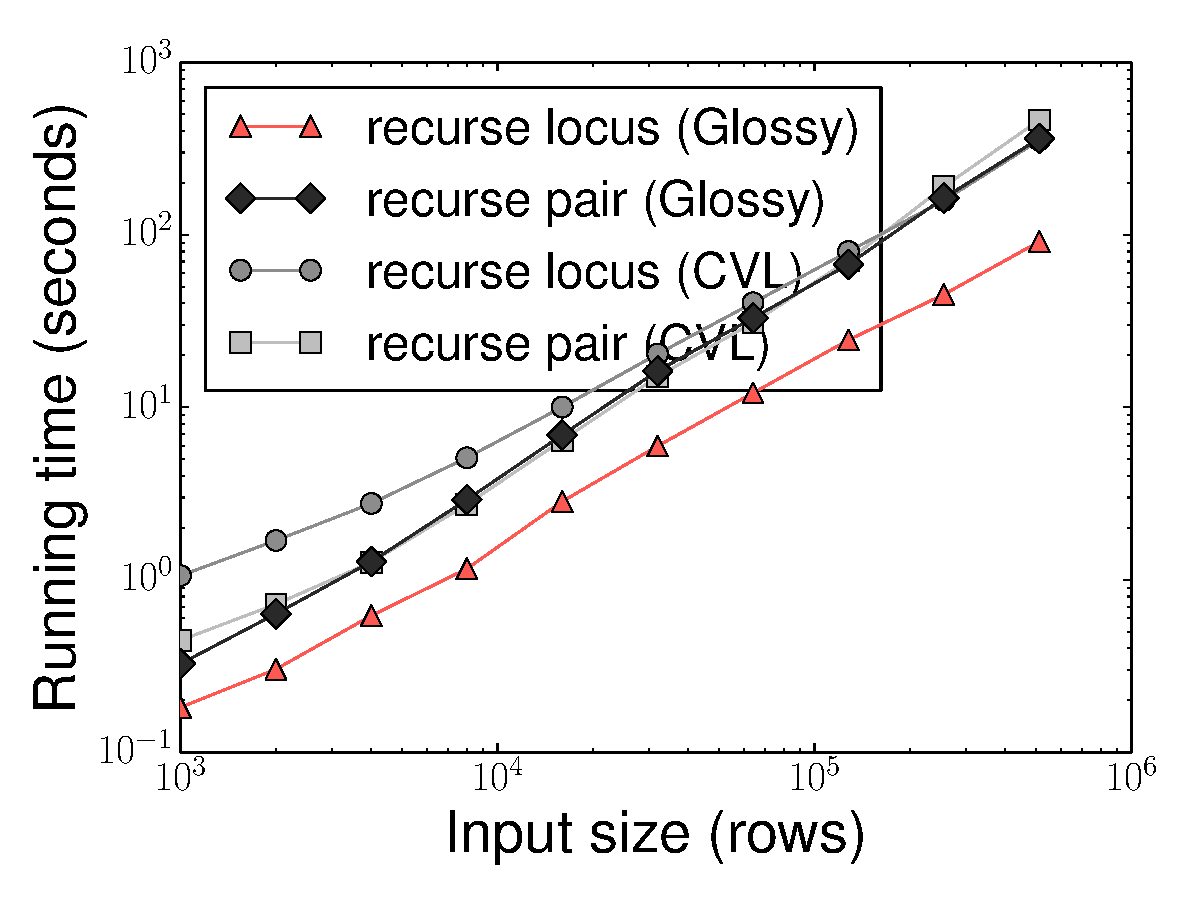
\includegraphics[width=1\linewidth]{figs-glossy/scalability_vs_cvl.pdf}}
        \vspace{-3ex}
        \caption{Scalability of equivalent recursive queries in Glossy vs. CVL with locus and pair constraints on scaled point of interest data.} \label{fig:scalability:glossy:vs:cvl}
    \end{minipage} \hfill
%\vspace{-1ex}
\end{figure*}

\subsection{Scalability}
\label{sec:exp:scalability}

We evaluated the scalability of Glossy SQL by deriving ten POI datasets with between $1000$ and $512000$ records, while attempting to scale dataset size exponentially. We adopt the same scaling procedure described by Kefaloukos et al.~\cite{KefaloukosSZ14:CVL}. A sweep-line approach is employed to enlarge the dataset along the x-axis in the west to east direction. The main property of this procedure is that the size of the dataset can be gradually increased, while maintaining local density. The scalability results are reported in Figure~\ref{fig:glossy:scalability}. 

To test a variety of queries, we started from the query of Figure~\ref{fig:glossy:sql:poi} and modified it along two dimensions: (a)~we chose to either use a single locus or pair constraint, and (b)~we chose to either use a \textbf{\texttt{RECURSE OVER}} or an \textbf{\texttt{ITERATE OVER}} clause. The four resulting queries were compiled by Glossy and executed on PostgreSQL. PostgreSQL failed to obtain an efficient query plan for the iterative query with a pair constraint. While the issue could potentially be addressed by manually adding optimizer hints or switching to a more sophisticated query optimizer, we preferred to  run the Glossy and PostgreSQL combination untouched in our experiments and thus omit the results for this particular query. 

Figure~\ref{fig:glossy:scalability} shows that the SQL queries generated by the Glossy SQL compiler scale linearly on the input size up to at least 510K data items. The figure also shows a marked difference between queries involving pair and locus constraints. The running times of the recursive query with a pair constraint are consistently worse than of the other two queries throughout the whole range of input sizes evaluated. With a dataset of $512000$ records, the observed response time is higher by a factor of roughly four, reaching close to seven minutes compared to just roughly two minutes for the other query types. The pair constraint involves a notoriously expensive spatial join operation, which we have confirmed to be the dominant factor in the observed differences. Note that Glossy SQL queries compute the entire visualization results for all zoom levels, so we argue that a response time of a few minutes is acceptable for the offline pre-computation of a whole visualization.     


\subsection{Running the Use Cases}

Having established the baseline scalability of SQL queries generated by Glossy, we turn our attention to the use cases discussed in Section~\ref{sec:use:cases} for which Glossy SQL queries have been presented in Section~\ref{sec:use:cases:solved}, Figures~\ref{fig:glossy:sql:rappers}-\ref{fig:glossy:sql:placenames}. We evaluate SQL queries generated by the Glossy SQL compiler over the real datasets of rap lyrics, points of interest, placenames, and the larger, synthetic placenames dataset. 

\begin{table}[ht]
%\vspace{-1ex}
\begin{center}
\tabcolsep=0.11cm
\begin{tabular}{|l|l|l|l|}
\hline
\multirow{2}{*}{\textbf{Use Case}} & \multirow{2}{*}{\textbf{Query}} & \multirow{2}{*}{\textbf{Dataset}} & \textbf{Response} \\
                                                             &                                                      &                                                          & \textbf{Time} \\ 
\hline
UC~\ref{ex:rappers}: Vocabulary Size & Figure~\ref{fig:glossy:sql:rappers} & Rap Lyrics & 157~msec  \\
UC~\ref{ex:poi}: Points of Interest & Figure~\ref{fig:glossy:sql:poi} & Points of Interest & 6.5~min  \\
UC~\ref{ex:placenames}: Placenames & Figure~\ref{fig:glossy:sql:placenames}\footnotemark & Placenames & 1.5~sec \\
UC~\ref{ex:placenames}: Placenames & Figure~\ref{fig:glossy:sql:placenames} & Synthetic Places & 6.6~min  \\
\hline
\end{tabular}
\vspace{-2ex}
\caption{Performance of running use cases with Glossy}
\label{tab:use:cases:performance}
\end{center}
\vspace{-3ex}
\end{table}%

The response times observed for running the use cases are summarized in Table~\ref{tab:use:cases:performance}. We observe that times are strongly correlated with input size and with the types and definitions of constraints employed by the queries. Use Case~\ref{ex:rappers} exhibits the lowest response time, of under a couple hundred milliseconds. This use case employs a Glossy SQL query with only a locus constraint, and is run over a relatively small dataset with $13000$ records. While Use Case~\ref{ex:placenames} is run over a comparatively small dataset, its query employs a locus constraint with more expensive geometric operations to obtain loci than the simple division of Use Case~\ref{ex:rappers}. This difference leads to an execution time roughly one order of magnitude larger. 

\footnotetext{Since the Placenames dataset from GeoNames only includes points, and not polygons for named places, we have changed the query in Figure~\ref{fig:glossy:sql:placenames} by omitting the \textbf{\texttt{WHERE}} clause, and by mapping each point to exactly one tile.}

In spite of the latter, execution times are still low in absolute terms for both small datasets. For the two larger datasets, we observe response times in the order of six to seven minutes. The behavior of Use Case~\ref{ex:poi} is in line with what we have observed in the scalability experiments of Section~\ref{sec:exp:scalability}, since the query employs a pair constraint with a spatial join. For Use Case~\ref{ex:placenames}, we again have the use of complex geometric operations, this time to determine tile centers for named place polygons over a challenging synthetic dataset. We speculate that the use of advanced methods for spatial operations in the underlying database, such as use of parallelism and advanced indexing structures, could speed these queries up by a substantial amount. 

\subsection{Comparison with CVL}

Over the previous sections, we have explored a range of queries and use cases for Glossy SQL. In this section, we focus on comparing Glossy SQL with CVL. Unlike Glossy SQL, CVL neither supports iterative queries nor the specification of an ordered table with information on scales. As such, we focus on recursive queries with range clauses over a fixed number of zoom levels. In addition, CVL requires specification of geometry columns, so we restrict our attention only to use cases in the domain of geographical maps. 

We compare the two systems with the POI and Placenames datasets evaluated previously, as well as the Airports dataset, which was used in the experimental evaluation of Kefaloukos et at.~\cite{KefaloukosSZ14:CVL}. We experiment with two types of recursive queries, namely containing either a single locus or pair constraint. All queries range over an interval of zoom levels $[0,18]$, similarly to Figure~\ref{fig:glossy:sql:poi}. 

Figures~\ref{fig:glossy:vs:cvl:locus} and~\ref{fig:glossy:vs:cvl:pair} show the results for both systems. We observe that for queries involving only a locus constraint, the performance of Glossy is substantially superior to that of CVL, exhibiting running times lower by over a factor of three. This result suggests that the SQL translation employed by Glossy for these queries is not only more general, but also more performant than the translation employed by CVL. For queries involving a pair constraint, however, the running time of both systems is comparable. This behavior is in line with our observation that the spatial join in the pair constraint essentially dominates the running time.        

To complete our evaluation, we have run a scalability experiment with the two systems, with a setup similar to the one of Section~\ref{sec:exp:scalability}. However, we focused only on the query types explored in this section, given the restrictions of CVL. The results are shown in Figure~\ref{fig:scalability:glossy:vs:cvl}. We can see that both systems scale linearly with the input size. That being said, we observe again in this experiment the performance trends above: For a locus constraint, the performance of Glossy is superior across the whole range of input sizes, while for a pair constraint involving a spatial join the performance of the two systems is comparable. 

From this evaluation, we observe that Glossy generally dominates CVL, not only in terms of expressivity, but also performance.  

% what to compare against?
% Selling points:
% - Global Selection: leaving minute data selection to system 
% Goal of experiment: Show that Global Selection can be implemented efficiently

\section{Conclusions}

In this paper, we argue for and propose an extension of SQL to express global selection operations, motivated by a wealth of use cases in data visualization. Global selections sample records from a dataset in a way that is at the same time constrained and weighted. The paper presents a concrete system, Glossy, that processes global selection queries by translating them to pure SQL and running the resulting queries over existing RDBMS. Glossy SQL allows for the declarative expression of both pair and locus constraints over the dataset, of a weighting function for records, and of both iterative and recursive global selections. The latter features let visualization developers express record importance as well as visual conflicts to be avoided in a manner sensitive to scale in a zoomable visualization. Experimental results with the Glossy SQL translation of several visualization use cases indicate that Glossy generates SQL code that an existing RDBMS can execute both efficiently and scalably with increasing input sizes. 

As future work, we plan to explore how to incorporate data aggregation features into Glossy SQL, as well as integrate Glossy with an existing library of visualization components such as D3.\footnote{http://d3js.org/}


\chapter{Tileheat: A Framework For Tile Selection}
\label{chapter:tileheat}
\section{Introduction}

% Situation
Today geospatial web services are widely deployed on the web. A significant subset of these services can be queried using bounding box requests to retrieve geospatial data, either in raster or vector form, within a region. The classic example of such a service is Web Map Service (WMS). In WMS, results are typically computed on-the-fly by pulling data from a geospatial database. This strategy has the advantage that results are always up-to-date and it thus offers a great degree of flexibility and accuracy to clients of the service. At a high level, we can think of the service as applying a \emph{rendering function} to a set of matched base data to produce, e.g., a map image.

% Problem
Services that apply rendering functions in response to bounding box requests are often CPU- and I/O-intensive, with relatively high latency as a consequence. This is a problem because geospatial services are typically used interactively, and latency in excess of a few hundreds of milliseconds becomes noticeable. Even if the computation is not that expensive, the infrastructure available might not scale to many simultaneous users, if data is to be computed on demand. We know from our studies of government production services that may use as much as 30 seconds to compute a 256 x 256 pixel map image, which severely lowers the value of the service in an interactive scenario. On the other side, limiting the use of GIS to working with results that can be computed fast, does not generally seem like a good idea. While the issue of high latency can to a certain degree be dealt with by scaling up or out, such solutions do not come without a cost, e.g. increased power consumption and hardware costs. Instead of simply adding more resources, better algorithms can be developed to deal with high latency.

% State of the art
Real-world workloads contain significant amounts of repeated requests and often a strong skew in what is requested~\cite{fisher07,talagala00}. This offers an opportunity to replay the results of previous computations by placing geospatial results in a cache. A common approach to representing a set of geospatial results at multiple resolutions is to use a tiling scheme that divides a geographical data set into a hierarchical and finite set of \emph{tiles}~\cite{decola93}. Unfortunately, the drawback of this approach is that the set of tiles is potentially very large~\cite{garcia11}, as the number of tiles is exponential in the number of supported resolutions. It is common to fix the number of resolutions when dealing with tiles, and thus we assume a fixed set of resolutions. Even then, the sheer number of tiles makes computing and storing all of them difficult to manage.

Two primary approaches have been suggested for dealing with the delivery of tiles to clients: \emph{online} and \emph{off-line}. The online approach attempts to mask the latency of computing tiles on-demand for a single user, by prefetching tiles based on predictions of future accesses given the user's current viewstate~\cite{KKK01:Prefetching,KKK01:Prefetching2,LKK+02:Prefetching}. The off-line approach is to materialize a large but polynomial number of tiles in advance that is expected to cover to the majority of user request in the near future. It is assumed that serving the materialized tiles from a cache will be less CPU- and I/O-intensive than computing them on demand. The main problem then becomes selecting a good set of tiles. 

A drawback to the online approach is that although pre-fetching theoretically masks latency for a single user, it does not by itself decrease global concurrency, as tiles are still computed on demand. We speculate that this approach could even increase the average latency if view states are mispredicted. A drawback with materializing a set of tiles offline is that the tiles might not be up-to-date by the time they are requested, but this can be solved by invalidating the stale tiles. We will focus on the latter off-line approach in our work.

The off-line approach takes a global view of the problem, and aims at predicting a ``good'' set of tiles, i.e., a set containing tiles that are likely to be requested by many users in the near future. We argue that these tiles should be materialized during a window of low load. This strategy avoids impacting latency negatively in the high load period, but holds the potential to reduce average latency because of pre-computation.

% which in turn increases the average global latency, in order to decrease the latency for a particular user. 
Methods in the literature use rule-based algorithms to select which tiles should be materialized ahead of time~\cite{quinn10}. The rules are based on \emph{a priori} knowledge of user behavior, so a drawback of these methods is that the rules do not adapt to changes in user behavior over time. In addition, rule-based methods are hard to adapt to shorter time windows of low load. As they offer only limited insight over which tiles are the most relevant among the tiles selected by the rules, it is hard to choose a good subset of tiles to be materialized under a time constraint.  
% MVS: are there other rule-based approaches that we can cite? Does anybody cite Quinn and Gahegan?

In this paper, we present an adaptive tile selection method, \emph{TileHeat}, which suffers significantly less from these drawbacks. TileHeat is based on  \emph{a posteriori} knowledge of user behavior gathered from historical usage of the geospatial web service. We investigate algorithms that predict the set of tiles that will be requested in time period $t + 1$, and that are trained using a log of requests for periods $t-n, t -n + 1, \ldots, t$. Our algorithms construct a set of $n$ spatial heatmaps of requests, one for each time period, and uses these to predict future requests. To avoid over-fitting the model to the training data, we use both exponential smoothing and heat dissipation on the constructed heatmaps. The output of our algorithms is a ranking of tiles based on predicted likelihood of access for the next time period. As such, the number of tiles to be pre-computed can be chosen according to the available time window of low load.	

\minisec{Outline and Contributions}
Our paper starts with a discussion of existing methodologies for tile caching (Section~\ref{sec:tile:caching}). Then the main \emph{contributions} of the paper follow:
%
\begin{itemize}

\item We analyze a sample from the production log of The Digital Map Supply, a production geospatial web service maintained by the National Survey and Cadastre (KMS) in Denmark. In Section~\ref{sec:analysis}, we present our key observations of the workload, e.g. that the load curve follows a pattern with high load in the middle of the day, and low load in the rest of the day, and that the spatial distribution of requests is very stable over time.

\item We present the general framework of TileHeat, and propose a set of algorithms for ranking tiles. The algorithms exploit the properties we have discovered in the analysis, namely by tracking and predicting the spatial distribution of requests using heatmaps (Section~\ref{sec:tileheat:algorithms}).

\item We present an experimental evaluation of the effectiveness of TileHeat. We observe an improvement of $25\%$ over the existing method used in the production system of KMS  for a set of tiles that can be materialized during an observed time window of low load (Section~\ref{sec:experiments}).

\end{itemize}
%
We end the paper by reviewing additional related work (Section~\ref{sec:tileheat:related:work}). 


\section{Background}
\label{sec:tile:caching}

A \emph{tile cache} is a widely used method for dealing with the bad performance of services that render results from base data on-the-fly, such as WMS and similar services. In the following, we discuss the main concepts (Sections~\ref{sec:tile:pyramid} to~\ref{sec:heatmap:model}) and existing methods (Section~\ref{sec:existing:methods}) in tile caching.

\subsection{The Tile Pyramid}
\label{sec:tile:pyramid}

Tile caches are based on a model called a \emph{tile pyramid}, which subdivides a geographical region into a finite number of subregions using a set of $l$ grids~\cite{decola93}. In Figure~\ref{fig:tilepyramid}, a tile pyramid with three levels is shown. The cells of the grids are called \emph{tiles}, and tiles are indexed by a triple $(i,j,z)$. In this triple $z$ identifies a grid, while $i$ and $j$ represent the row and column in the grid where the tile is located. Each grid is associated with a data set at a particular resolution in meters per pixel. Tiles thus correspond to data at a given resolution, and within a bounding box.

\begin{figure}
\centering
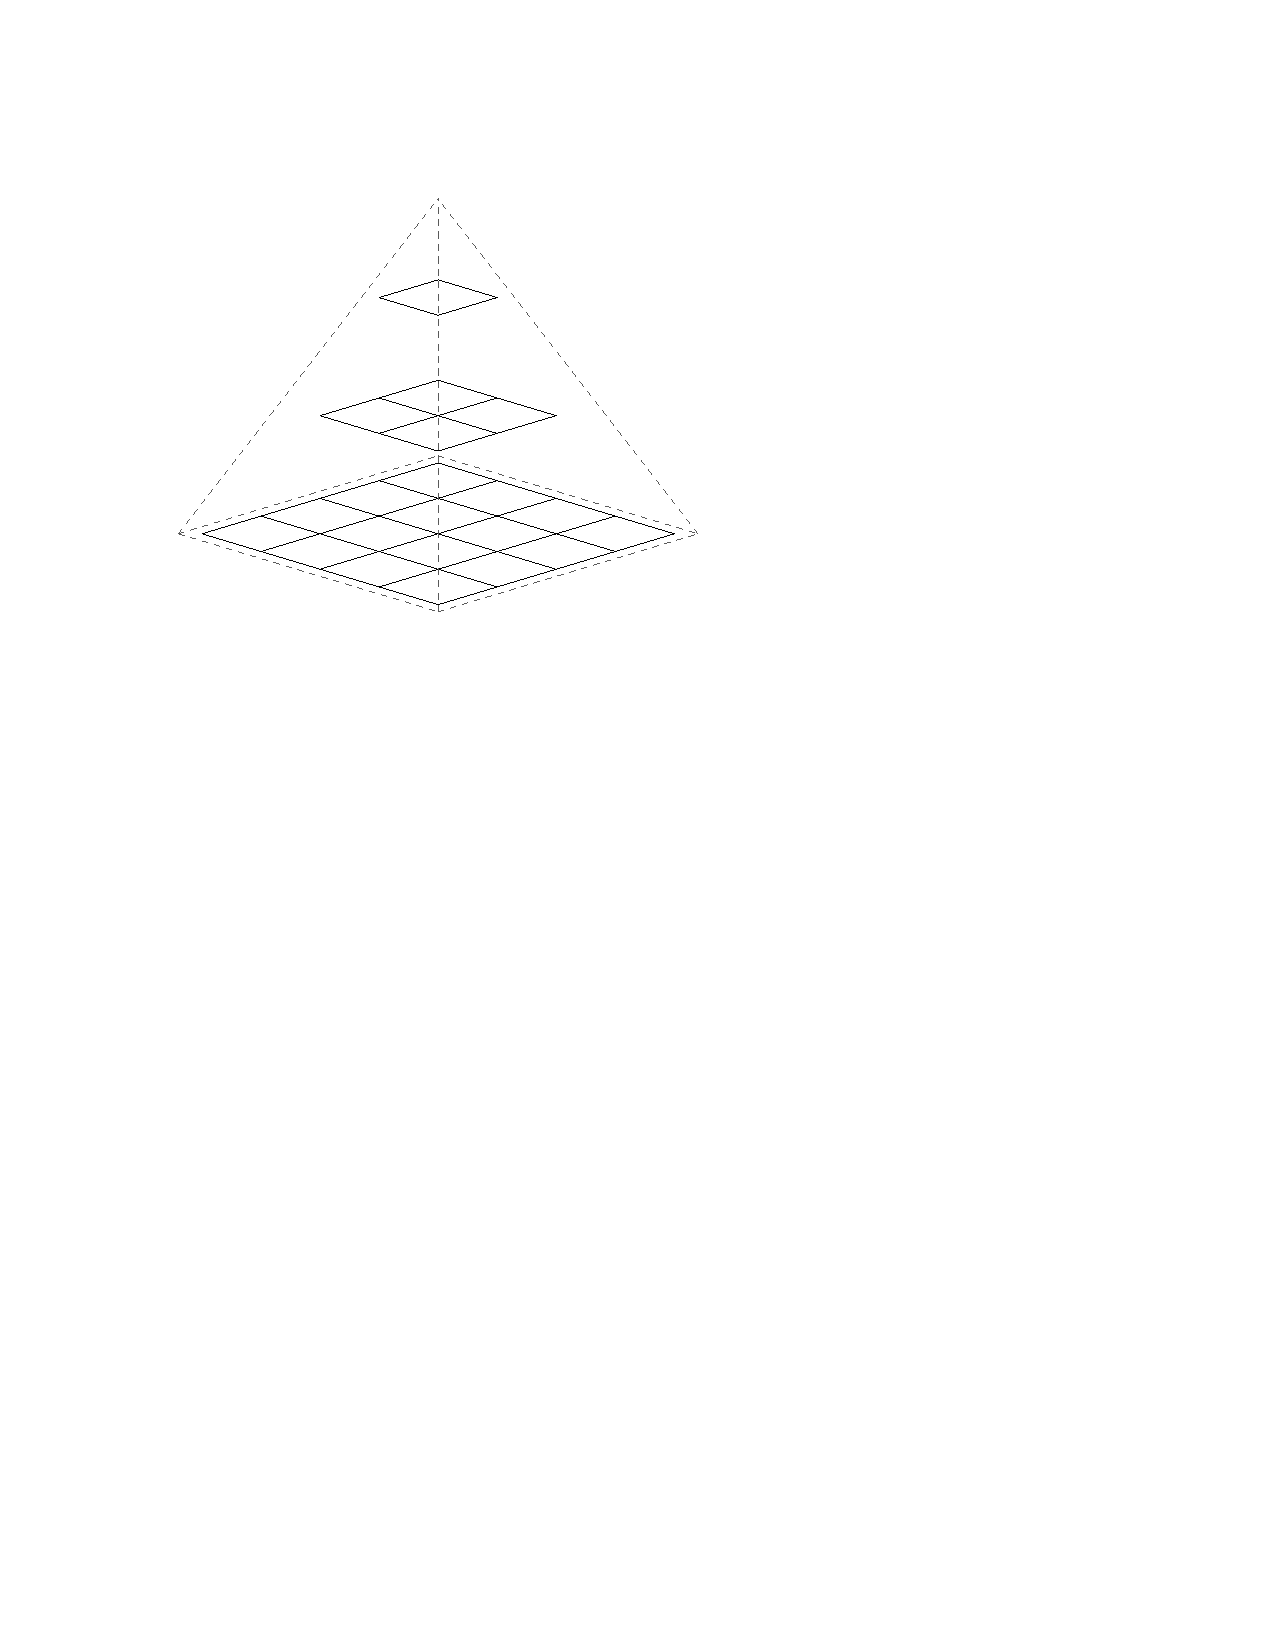
\includegraphics[scale=0.8]{figs-tileheat/tilepyramid}
\caption{Tile pyramid with three levels $z=\{1, 2, 3\}$ shown. Level $z=1$ has dimensions $(1,1)$. Figure is reproduced from \cite{quinn10}}
\label{fig:tilepyramid}
\end{figure}

When a tile cache is initialized, all tiles point to $null$. A tile is materialized by making it point to geographical data stored on disk. The geographical data is rendered from a set of base objects, and if the base objects are updated the tile becomes \emph{stale}. Stale tiles are removed to avoid serving stale data to clients.

One shortcoming of tile caches is that the number of tiles is exponential in $l$, with grid $i+1$ containing four times as many tiles as grid $i$. This means that a tile cache consumes $O(4^l)$ in storage, and $O(4^l)$ time is required to materialize all tiles. A pyramid of $l=20$ levels requires several petabytes of storage \cite{garcia11}. The throughput of computing tiles has been reported by KMS to be around $58$ tiles per second on their infrastructure \cite{lindegaard12}. At this rate of computing tiles, it would take approximately $200$ years to compute the $3.7 \times 10^{11}$ tiles needed~\cite{garcia11}.

\subsection{Processing user requests}
\label{sec:processing:user:requests}
We abstract user requests to a geospatial web service by two functions: \texttt{GET} and \texttt{PUT}. \texttt{GET} retrieves a tile from a web service, while \texttt{PUT} updates the base data from which tiles are computed. Pseudocode for processing \texttt{GET} and \texttt{PUT} requests are given in Figure \ref{fig:pseudocode}.

\begin{figure}[ht]
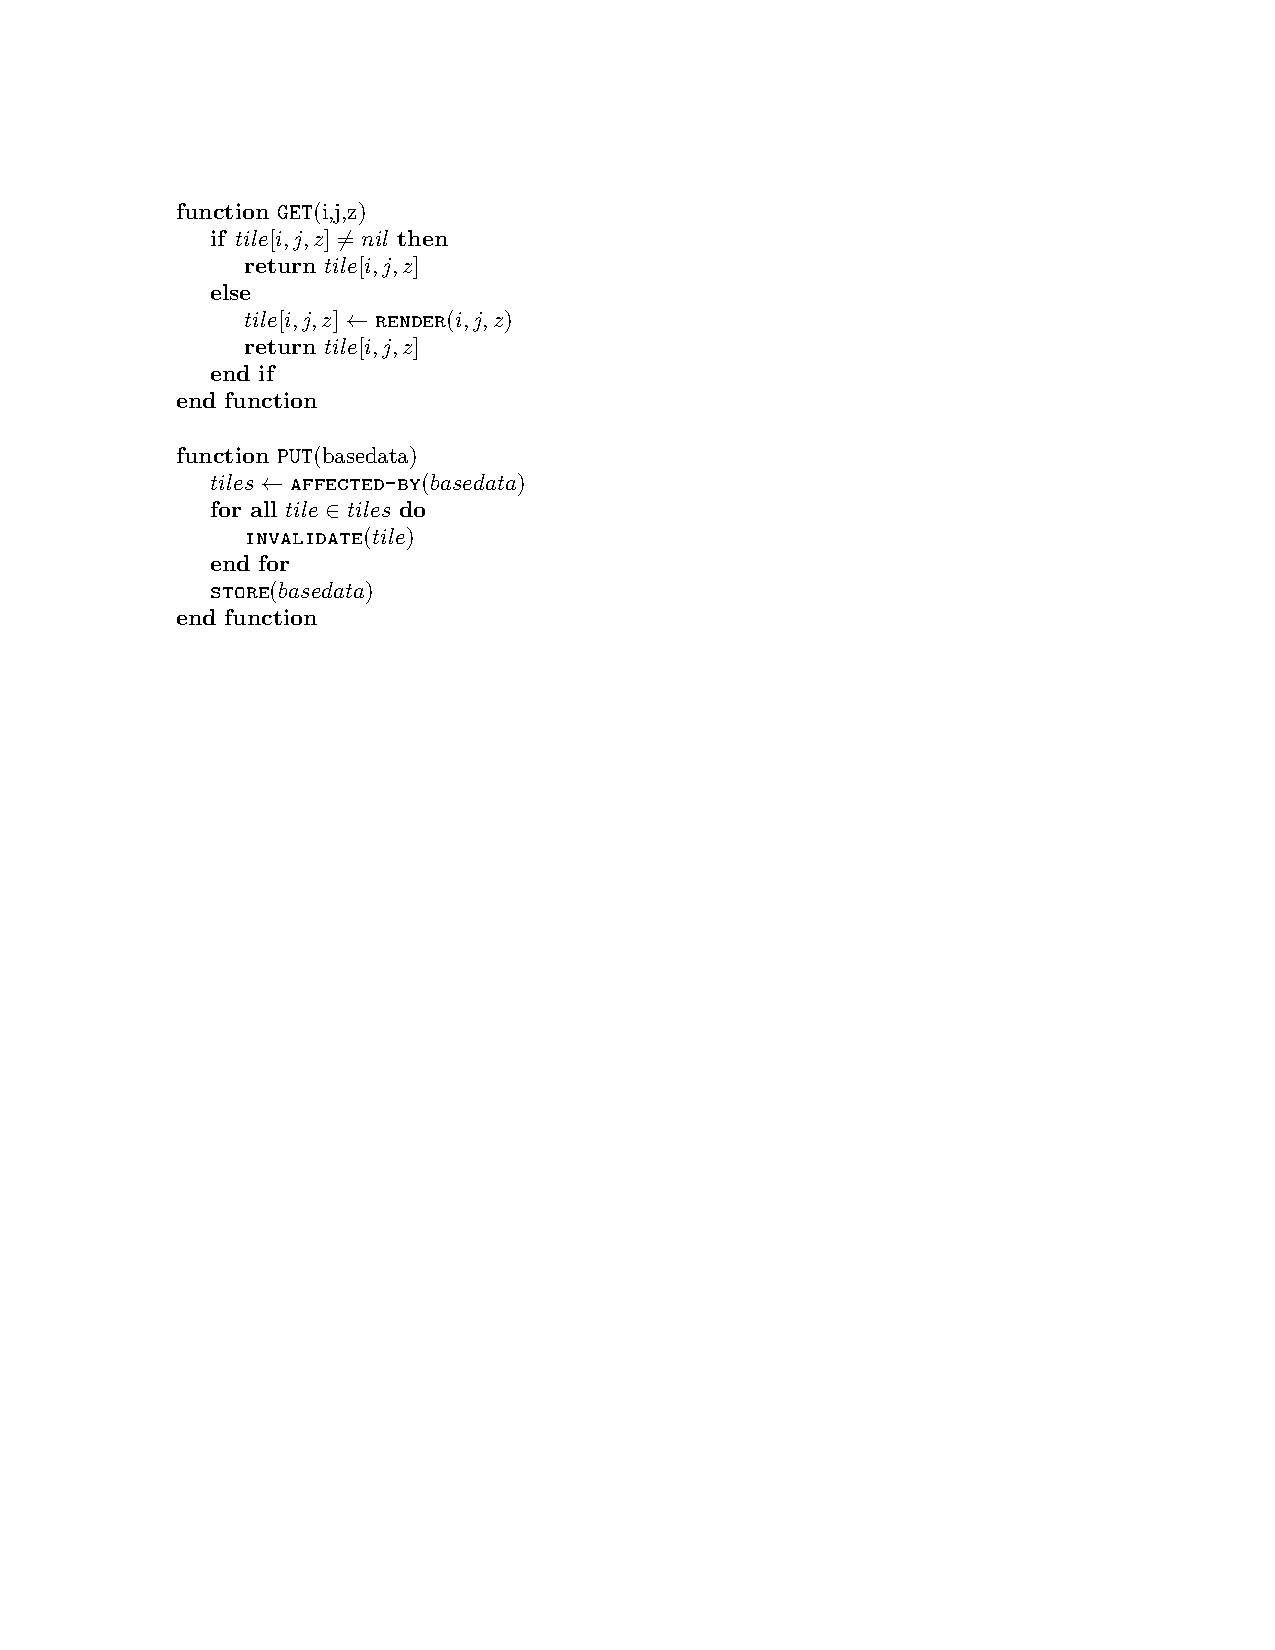
\includegraphics[scale=0.9]{figs-tileheat/pseudocode}
\caption{Processing a \texttt{GET} request: If the tile is materialized, it is returned. Otherwise it is rendered, stored and returned. Processing a \texttt{PUT} request: When base data is updated, the set of tiles that is affected by the change needs to be invalidated.}
\label{fig:pseudocode}
\end{figure}

An invariant maintained by the above functions is that stale tiles are never returned to the user. However, one implementation difficulty typically encountered in practice is that the method for determining the set of tiles that are affected by an update to the base data is not entirely accurate, i.e., a conservative estimate is used in function \texttt{AFFECTED-BY}. This means that sometimes tiles are unnecessarily discarded.

A bounding box request, such as a WMS request, can easily be modeled as a set of \texttt{GET} requests by computing the set of tiles that are intersected inside the \emph{nearest} grid of the tile pyramid. By nearest, we mean the grid that contains tiles with a resolution that best matches the resolution of the bounding box request. Note that these multiple \texttt{GET} requests must be processed against a consistent snapshot. 
%Description of the appropriate implementation details are however beyond the scope of this paper. 

\subsection{The Heatmap model}
\label{sec:heatmap:model}
Given a set of \texttt{GET} requests, we can generate a heatmap of the requests \cite{fisher07}. A heatmap quantifies the number of requests $h_{i,j,z}^t$ that a tile with index $(i,j,z)$ has received in time period $t$. We consider multi-scale heatmaps, which are associated with a tile pyramid. In this work, we only use heatmaps to measure the number of \texttt{GET} requests per tile, but other request types could also be tracked with heatmaps. For example, we could generate heatmaps of \texttt{INVALIDATE} requests, but this is outside the scope of our work.

\subsection{Existing Methods}
\label{sec:existing:methods}
This section covers existing methods for computing and storing a set of tiles for a tile cache.

\minisec{Parallel processing}
Clearly, we need techniques to speed the computation of a tile cache up, given that the number of tiles in a tile pyramid is huge. Using a parallel programming model such as MapReduce \cite{dean04} could reduce computation time of a tile cache by a large factor, but it would require a significant number of machines. In other words, parallelism improves time-to-solution, but does not reduce the amount of resources necessary for the computation. For organizations such as KMS, this high resource cost renders the use of brute-force parallelism unfeasible. A solution is called for to reduce the number of tiles that needs to be computed --- which could then be orthogonally combined with parallelism if available.

\minisec{Detecting duplicates}
A method that reduces storage requirements is to exploit that many tiles are identical, e.g., blue ocean tiles~\cite{mbtile12}. Unfortunately, this solution does not necessarily reduce computation time, given that tiles often must be computed in order to check that they are duplicates. Heuristics have been suggested to predict these duplicated tiles without full computation, but it is unfortunately not easy to decide with absolute certainty~\cite{mbtile12}. We do not know of any published methods that accurately and efficiently predict whether two tiles are the same in the general case without actually computing them, because arbitrary rendering functions are employed.

\minisec{Tile Caching based on Geometries}
A number of authors have suggested methods for predicting the popularity of tiles. Quinn and Gahegan~\cite{quinn10} suggest using certain classes of base objects, like roads and coastlines, as predictors of where people will look at a map. Tiles that are at most 3 miles away from the selected predictors are cached. Conceptually, this approach is based on a model of rational user behavior with fixed rules, and historical workloads are used only to validate the model.

\minisec{GEOM}
KMS currently uses a simplified version of the approach above, which we term \emph{GEOM}. A set of polygons that roughly cover the land areas of Denmark are used to identify the areas that should be fully materialized at all levels of the tile pyramid (levels 1 to 12). Areas outside of these polygons are only materialized at the top-most levels of the tile pyramid (levels 1 to 6)~\cite{lindegaard12}. The resulting partial cache is manageable in size, as roughly $10\%$ of the tile pyramid is materialized. However, the computation time is reported to be between $1.5$ and $2$ days. Tiles are generated by going row-by-row down the levels of the tile pyramid. This is significantly better than random selection, as the highly popular tiles near the top of the pyramid are generated early.

\section{Analysis}
\label{sec:analysis}

In this section, we analyze the request log of a production geospatial web service within KMS, and observe a number of interesting patterns.
The service we examine is the most popular web service of the The Digital Map Supply, a WMS that receives around 800,000 requests per day, and delivers a general purpose background map of Denmark. We report on both temporal (Section~\ref{sec:temporal:characteristics}) and spatial (Section~\ref{sec:spatial:characteristics}) characteristics of the workload.

\subsection{Temporal characteristics of workload}
\label{sec:temporal:characteristics}

\begin{figure}
\centering
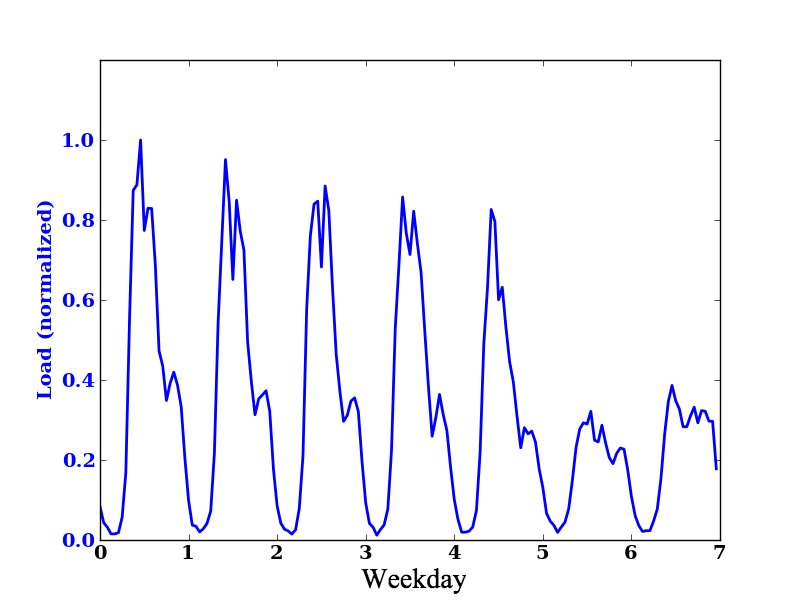
\includegraphics[scale=0.5]{figs-tileheat/average_load_week.png}
\caption{Average load per hour for each day of the week in the Digital Map Supply.}
\label{fig:weekload}
\end{figure}

Using a random sample of 90,000 WMS requests from the log, we analyze the workload over time. We have found the following when examining requests processed per second:

\begin{itemize}
\item The load is consistently higher during the middle part of the day, than during other parts of the day.
\item The 24-hour load curves for any two weekdays are very similar.
\item The 24-hour load curves for Saturdays and Sundays are very similar.
\item In general, the load is much higher during weekdays, compared to weekends.
\end{itemize}

These patterns are shown in Figure~\ref{fig:weekload}, where we display the average 24-hour load curve for each day of the week. The curve is generated as an average of all weeks in the log.

\begin{figure}
\centering
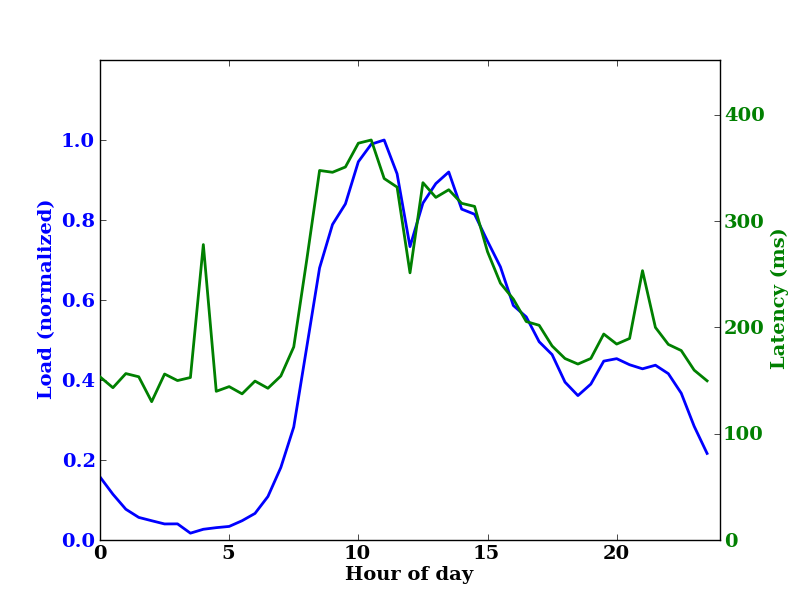
\includegraphics[scale=0.5]{figs-tileheat/correlation.png}
\caption{Correlation between average load (blue) and average latency (green) in the Digital Map Supply.}
\label{fig:correlation}
\end{figure}

We have also looked at the effect of load on latency. In Figure~\ref{fig:correlation}, we plot, side-by-side, the average load and latency curves for a 24-hour period. We observe the following:

\begin{itemize}
\item Load and latency are highly correlated, especially during the periods of high load.
\item The latency effectively doubles when the load is high.
\item Given that weekdays have higher load than weekends, the degradation of latency is most severe in the middle of the day, on weekdays.
\end{itemize}

Our hypothesis is that the increase in latency is caused by increased concurrency and queueing in the system. We have also tested the stability of the load pattern over time by plotting the load for each day over a longer period within the last quarter of 2011. The load patterns can be seen in Figure~\ref{fig:anomaly}. We observe that in general the load curve is very consistent from one weekday to the next, and one week to the next, but anomalies do occur. During week 49 of the last quarter of 2011, the number of requests suddenly doubles. While it is not easy to know what caused such a load spike, it is interesting to ask whether the spike affects the spatial distribution of requests. We examine this question in Section~\ref{sec:spatial:characteristics}.

\begin{figure}
\centering
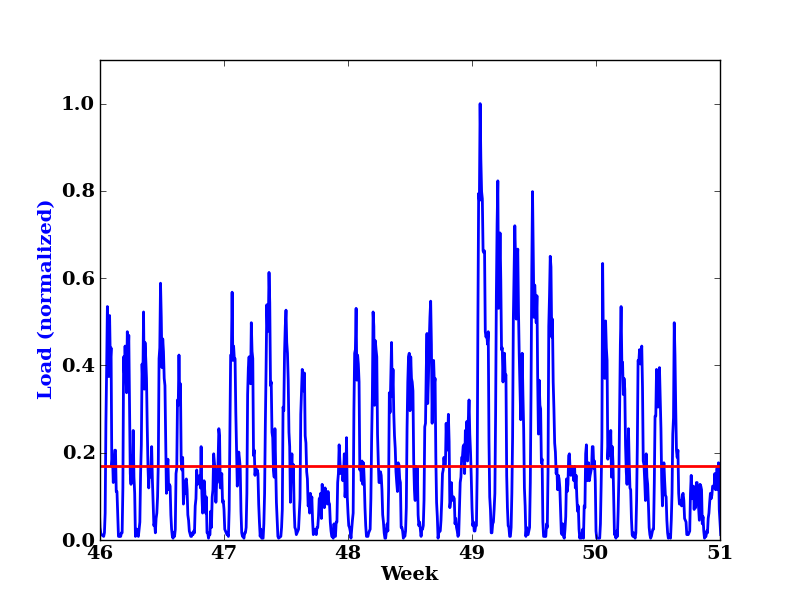
\includegraphics[scale=0.5]{figs-tileheat/anomaly.png}
\caption{In the Digital Map Supply, the loads for consecutive weeks generally resemble each other. However, week 49 exhibits an anomaly; the high load was caused by a big project in the public sector, which used data from the Digital Map Supply. The red line shows the average load.}
\label{fig:anomaly}
\end{figure}

\subsection{Spatial characteristics of workload}
\label{sec:spatial:characteristics}
Using heatmaps we have investigated the spatial distribution of requests. We have selected a large number of weekdays, and extracted a full log for these days. The number of log records is significant, with more than 800,000 requests received per day. In Figure \ref{fig:heatmaps}, we show heatmaps for four of these days. We observe that the spatial distribution of requests is quite similar across days. We observe a similar pattern on other days from the log that we have examined.

Given the anomaly in requests per second that we noted in Figure~\ref{fig:anomaly}, we wanted to investigate if the spatial distribution of requests was different for days of increased load compared to normal days. The lower right part of Figure~\ref{fig:heatmaps} shows a heatmap for the day with unusually high load. The spatial distribution is slightly different compared to the other three heatmaps, but still very similar. The data indicates that the spatial distribution of requests is similar for weekdays, and largely independent of fluctuations in load. Using the notation we defined for heatmaps this means that

\[
h_{i,j,z}^t \approx h_{i,j,z}^{t+1}
\]

\begin{figure}
\centering
\begin{tabular}{cc}
%\hline
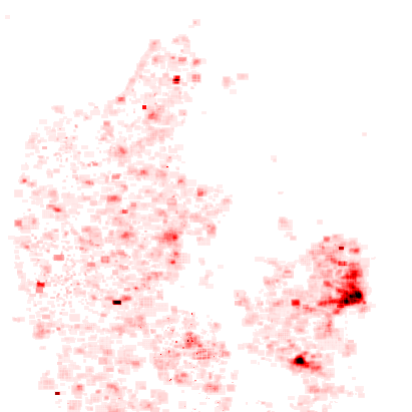
\includegraphics[scale=0.5]{figs-tileheat/heatmap-e_1.png} & 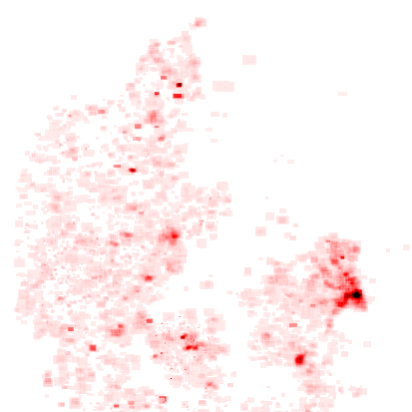
\includegraphics[scale=0.5]{figs-tileheat/heatmap-e_2.png} \\
%\hline
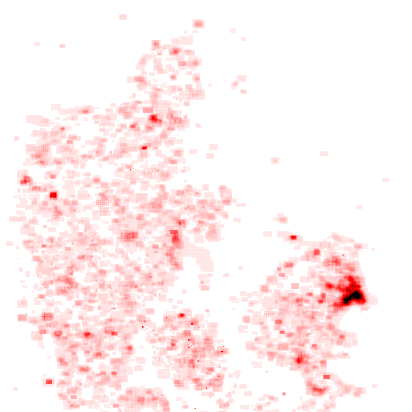
\includegraphics[scale=0.5]{figs-tileheat/heatmap-e_3.png} & 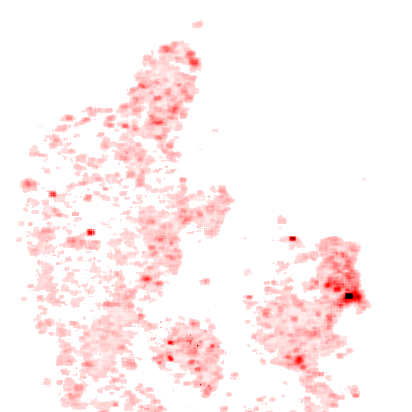
\includegraphics[scale=0.5]{figs-tileheat/heatmap-e_4.png} \\
%\hline
\end{tabular}
\caption{Four heatmaps showing the areas in Denmark most viewed on maps from the Digital Map Supply on four consecutive days (resolution $\mathbf{3.2}$ meter/pixel). The day in the lower right corner is the day with very high load identified in Figure \ref{fig:anomaly}.}
\label{fig:heatmaps}
\end{figure}

%In Figure~\ref{fig:skew}, we show the cumulative distribution function of tile access frequencies, which has been computed from the heatmaps. 
We observe that the frequency of tile access is highly skewed; other studies have concluded the same, namely that the spatial distribution of \texttt{GET} requests follows a power law \cite{fisher07,talagala00}. We also observe that the skew increases with resolution, i.e., with  levels of the tile pyramid that contain more tiles. 

In general, this means that the set of tiles needed for a tile cache with a high hit ratio is smaller than one might expect. The main goal of our work and the algorithms we have developed is to explore how small such a cache can be, while still delivering high hit ratios on user requests.

\section{TileHeat framework}
\label{sec:tileheat:algorithms}

In this section, we present the TileHeat framework for selecting and caching tiles. We begin with an overview of the framework and the context it is used in (Sections~\ref{sec:tileheat:overview} and~\ref{sec:tileheat:tasks}), followed by two different algorithms for tile ranking (Sections~\ref{sec:heat:hw} and~\ref{sec:heat:d}).   

\subsection{Overview}
\label{sec:tileheat:overview}
Based on our observations of the workload in Section \ref{sec:analysis}, we have designed the TileHeat framework for a repeated cycle of time periods containing a high- and low-load window. This basic cycle is outlined in Figure~\ref{fig:high:low}.

The life cycle of a system that uses TileHeat to manage tiles is as follows: We organize processing in TileHeat into a sequence of \emph{time periods}. Each time period is composed of two \emph{time windows}: the high-load window and the low-load window. Throughout both windows, the geospatial web service is available for clients and therefore must carry out normal processing of user requests, i.e., \texttt{GET} and \texttt{PUT}. During the low load window, however, we can additionally \emph{select and pre-compute tiles} that we expect to be accessed during the next time window, based on access patterns observed for previous time periods. In the following, we describe how we carry out the selection and pre-computation of tiles.

\begin{figure}
\centering
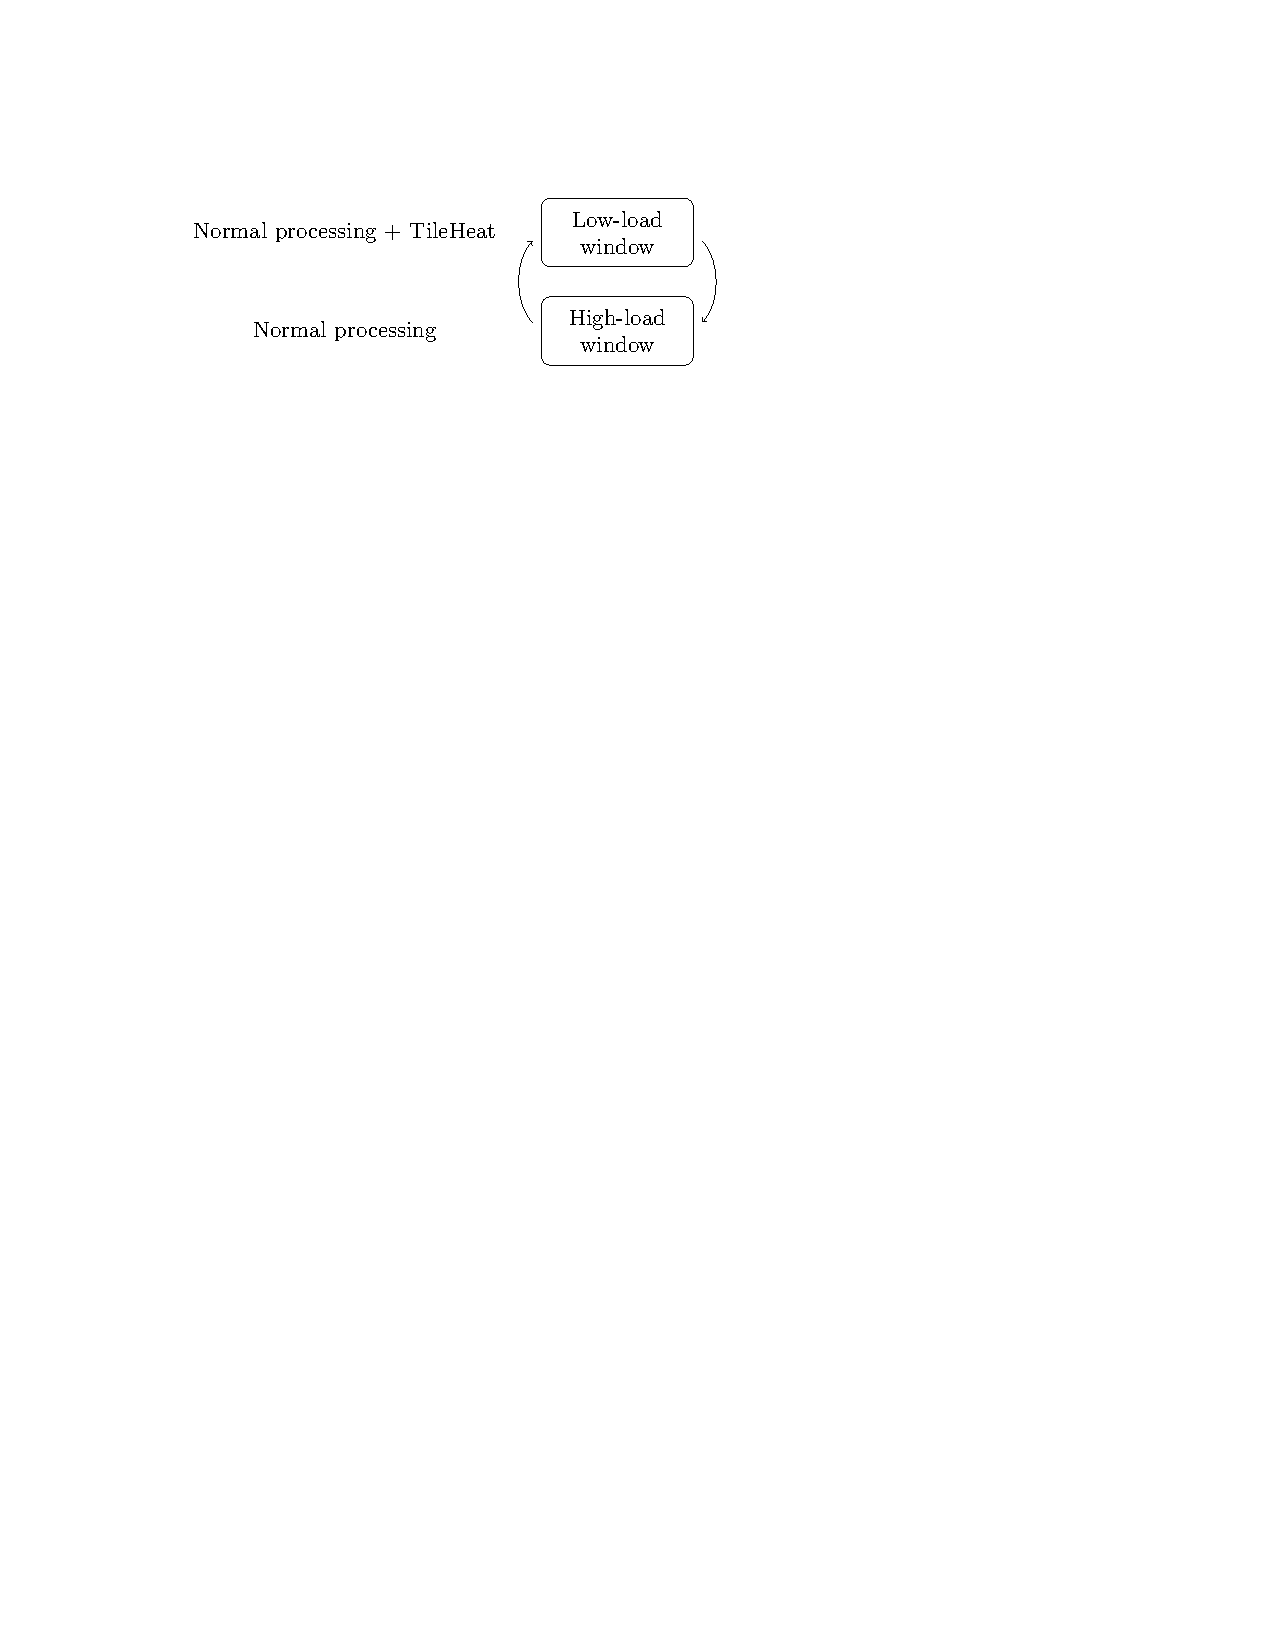
\includegraphics[scale=0.8]{figs-tileheat/figoverview}
\caption{Time periods and time windows: Processing during high- and low-load windows.}
\label{fig:high:low}
\end{figure}

%We assume that the base data from which the tiles are generated, gets updated frequently, which makes it a bad strategy to compute the entire set of tiles. 

\subsection{Tasks performed by TileHeat}
\label{sec:tileheat:tasks}

TileHeat is a framework for embedding tile selection algorithms into a log analysis procedure. The log analysis procedure computes a set of $n$ heatmaps, and passes these to tile selection. Tile selection in turn employs a \emph{prediction algorithm}, which predicts the heatmap for time $t + 1$. TileHeat uses the predicted heatmap to select which tiles to materialize for the next high-load window. 

The following steps are performed in time period $t+1$ by the TileHeat framework:
%
\begin{enumerate}
\item A prediction algorithm uses heatmaps for time periods $t-n$ to $t$ to predict the heatmap for time period $t+1$.
\item The tiles in the predicted heatmap are sorted in non-increasing order by heat.
\item The $k$ first tiles that are not already materialized are selected.
\item The materialization of the $k$ tiles is scheduled.
\end{enumerate}

The number $k$ is chosen as the number of tiles that can be materialized during the current low-load window. Various algorithms can be used to predict the heatmap for $t + 1$. In this work, we present two algorithms for the TileHeat framework: HEAT-HW (Section~\ref{sec:heat:hw}) and HEAT-D (Section~\ref{sec:heat:d}).

The running time of TileHeat can be estimated as follows. Let $m$ be the number of requests in the request log for time periods $t-n$ to $t$. We assume that the number of \texttt{GET} requests for each log request is bounded by a constant. The number of tile requests is therefore $O(m)$. By using a hash table, we can build the heatmaps in (expected) $O(m)$ time. As the sorting step takes at most $O(m)$ tiles as input, the (expected) running time of TileHeat is $O(m \log m)$ --- plus the running time of the prediction algorithm. 

\subsection{HEAT-HW algorithm}
\label{sec:heat:hw}
We have developed the HEAT-HW algorithm, which uses exponential smoothing applied to the heatmaps for time periods $t-n$ to $t$. Specifically, we use Holt-Winter double exponential smoothing~\cite{chatfield88}, which takes the trend of the observed variable into account. We motivate our choice of smoothing function in two ways:

\begin{enumerate}
\item We apply a smoothing function in general to avoid overfitting to the training data. Although the data we have analyzed is very stable, we introduce smoothing to prepare the algorithm for less stable workloads.
\item We use Holt-Winter smoothing in particular because it captures the trend in popularity for each tile. In future work, we would like to make use of the trend to adapt proactively to sudden rises in popularity for a geographical subregion by increasing the number of nodes serving those tiles. This of course implies a multi-node cache.
\end{enumerate}

Exponential smoothing is applied by treating each heat tile index $(i,j,z)$ as a separate variable. The equations for double exponential smoothing for heatmaps are given below (assuming that the first time period is $0$).

\begin{eqnarray*}
s_{i,j,z}^0 & = & h_{i,j,z}^0 \\
b_{i,j,z}^0 & = & h_{i,j,z}^1 - h_{i,j,z}^0 \\
s_{i,j,z}^{t+1} & = & \alpha h_{i,j,z}^0 + (1 - \alpha)(s_{i,j,z}^{t} + b_{i,j,z}^{t} ) \\
b_{i,j,z}^{t+1} & = & \beta (s_{i,j,z}^{t+1} - s_{i,j,z}^{t}) + (1 - \beta) b_{i,j,z}^{t}  \\
\end{eqnarray*}

As defined in Section~\ref{sec:heatmap:model}, $h_{i,j,z}^t$ is the observed heat of tile $(i,j,z)$ in time period $t$; $s_{i,j,z}^t$ is the smoothed value for time $t$ and $b_{i,j,z}^t$ is the trend for time $t$. Parameters $\alpha$ and $\beta$ are determined experimentally.

\subsection{HEAT-D algorithm}
\label{sec:heat:d}
The exponential smoothing as used in HEAT-HW only ranks tiles that are actually requested in the training data. Often, the training data is sparse, or tiles that are not accessed in the time periods $t-n$ to $t$ get accessed in time $t+1$, due to local changes in the spatial distribution of tile requests. 

HEAT-D is inspired by Tobler's first law of geography: ``Everything is related to everything else, but near things are more related than distant things''. HEAT-D works by applying a dissipation step to all heatmaps prior to applying Holt-Winter double exponential smoothing. The dissipation step is similar to the Jacobi method used for numerically solving the heat equation~\cite{templates}.

The following steps are performed by HEAT-D: 

\begin{enumerate}

\item For each heatmap of time periods $t-n$ to $t$, apply $p$ iterations of the dissipation step. An iteration consists of moving a fraction of the heat of each cell $(i,j,z)$ to its eight neighbors. This fraction is controlled by  a dissipation constant $\mu$. The corresponding differences in heat applied to each cell are shown in Figure~\ref{fig:dissipate}. 

\item Apply HEAT-HW over the heatmaps obtained in the step above. 

\end{enumerate}

%We apply $p$ rounds of the dissipation step to each heatmap in the training data. For each index $(i,j,z)$ in the heatmap, the dissipation step moves a fraction of the heat for that tile to its eight neighbors, based on a dissipation constant $\mu$. The process is illustrated in Figure~\ref{fig:dissipate}.

\begin{figure}
\centering
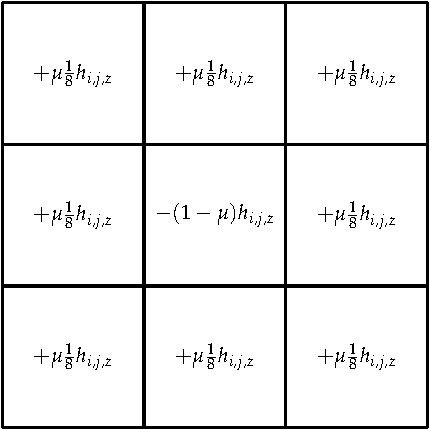
\includegraphics[scale=1]{figs-tileheat/disspate2}
\caption{Each dissipation step transfers heat from a center cell to each of it's eight neighbors. The center cell $(i,j,z)$ loses $(1 - \mu) h_{i,j,z}$ heat, and the neighbors gain $\mu \frac{1}{8} h_(i,j,z)$ heat. This is repeated for all center cells that are not on the border of the heatmap, using double buffering to avoid prematurely updating the heat of a cell.}
\label{fig:dissipate}
\end{figure}

The result of running dissipation on a sparse sample set can be seen in Figure~\ref{fig:dissipate_before_after}.

\begin{figure*}
\centering
\begin{tabular}{ll}
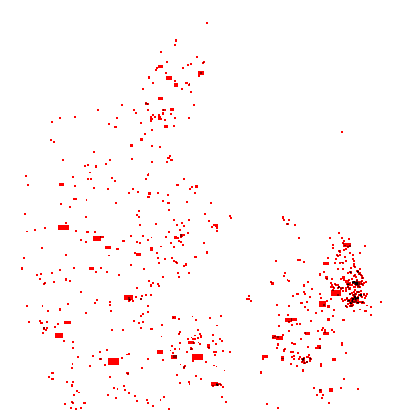
\includegraphics[scale=0.5]{figs-tileheat/heat_d-before.png} & 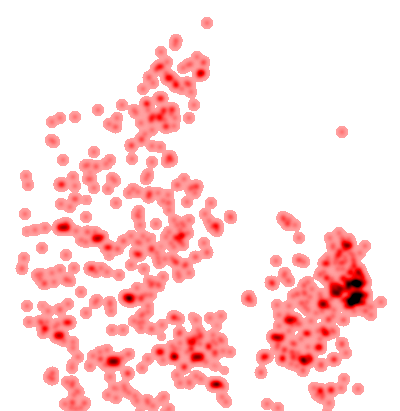
\includegraphics[scale=0.5]{figs-tileheat/heat_d-after.png} \\
\end{tabular}
\caption{Result of running the dissipation algorithm on a sparse heatmap (left) which contains $1.25\%$ of the samples used to create the heatmaps of Figure~\ref{fig:heatmaps}. The result (right) covers the hot regions of the heatmaps in Figure~\ref{fig:heatmaps} much better.}
\label{fig:dissipate_before_after}
\end{figure*}

\section{Experiments}
\label{sec:experiments}

The goal of our experiments is to show the improvements that can be gained by TileHeat in real production workloads. We first describe our experimental setup (Section~\ref{sec:setup}) and then present results (Section~\ref{sec:results}).  
%in a real production setting. We use real production workloads to test the hit ratio of the selected tile sets. 

\subsection{Experimental setup}
\label{sec:setup}

Here we describe how we have executed the experimental evaluation of our algorithms using a production request log extracted from KMS. Due to constraints in both time and access to the production system, we have not actually materialized the tiles selected by our methods, so we could not measure the effect this would have on latency in a production environment. Assuming, however, that serving tiles from cache is much more CPU- and I/O-efficient than computing on demand, we believe that the effect would be significant, given the high hit ratios we are able to achieve (Section~\ref{sec:results}). 

\subsubsection{Datasets}
\label{sec:datasets}
To validate the algorithms we have developed, we have extracted six datasets from the KMS request log for the last quarter of 2011. The method we used was to randomly select six weekdays, and for each of these days, select the $n$ previous weekdays to be used as training data. We use $n=3$. 

%Each dataset thus consists of the following:
%
%\begin{itemize}
%\item One weekday to use for validation.
%\item Three previous weekdays to use as training data. 
%\end{itemize}

The size of the log of requests for each weekday is substantial, with over 800,000 WMS requests per day, which we translate into \texttt{GET} requests. 

\subsubsection{Methodology}
\label{sec:methods}

This section describes our experimental methodology. The algorithms we have tested are:

\begin{itemize}

\item OPT: the optimal algorithm, which builds a heatmap of the workload used for the validation, and uses this heatmap to select the tiles. 

\item GEOM: the method currently employed by KMS, described in Section~\ref{sec:existing:methods}.

\item HEAT-HW: our heatmap method with Holt-Winter double exponential smoothing, described in Section~\ref{sec:heat:hw}. For HEAT-HW, the best set of parameters we could devise was $\alpha = 0.2$ and $\beta = 0.1$. 

\item HEAT-D: our heatmap method extended with dissipation, described in Section~\ref{sec:heat:d}. For HEAT-D, we set $\mu = 0.05$. The number of iterations $p$ is calibrated according to the resolution of the heatmap being dissipated. Given a scale factor $s$, we set $p = s \times (\text{\#rows}+\text{\#columns})/2$. The intuition is that heatmaps with higher resolution need more iterations of the dissipation step in order to cover enough geographical area. We set $s = 0.002$. 

\end{itemize}

The methodology we have developed to test the algorithms consists of playing back the production request log, both to train the algorithms, and to validate their performance. The outline of the method is as follows:

\begin{enumerate}
\item Pick a random day $t$.
\item Compute $n$ heatmaps for the $n$ consecutive days leading up to and including $t$.
\item Compute the actual heatmap for day $t+1$ from the data. 
\item Normalize the cells of the actual heatmap for day $t+1$ by the sum of heat for all cells. Now, each cell in the actual heatmap contains the fraction of the hit ratio contributed by the corresponding tile for day $t+1$. 
\item Calculate the tile ranking for the OPT algorithm by sorting tiles according to normalized heat contained in the actual heatmap.
\item For each of the other algorithms, obtain the corresponding tile ranking for day $t+1$, and measure the hit ratio by cumulating normalized heat from the actual heatmap.    
%\item The $n$ heatmaps are given as input to the algorithms GEOM, HEAT-HW, HEAT-D, and the output consists of the corresponding predictions of the heatmap for day $t+1$.
%\item Independently sort the cells of the two predicted heatmaps by decreasing heat, obtaining two lists of sorted cells.
%\item For each list, iterate over the cells, starting with the cell with highest heat. For each cell, look up the heat of the corresponding cell in the actual heatmap for day $t+1$, and plot these heat values cumulatively.
\end{enumerate}


Our results show averages of the hit ratios obtained by running the algorithms against each of the six datasets, recalling that a dataset consists of three days used to train the algorithms, and one day used to validate the performance of the algorithm.

\subsection{Results}
\label{sec:results}

\begin{figure*}
\centering
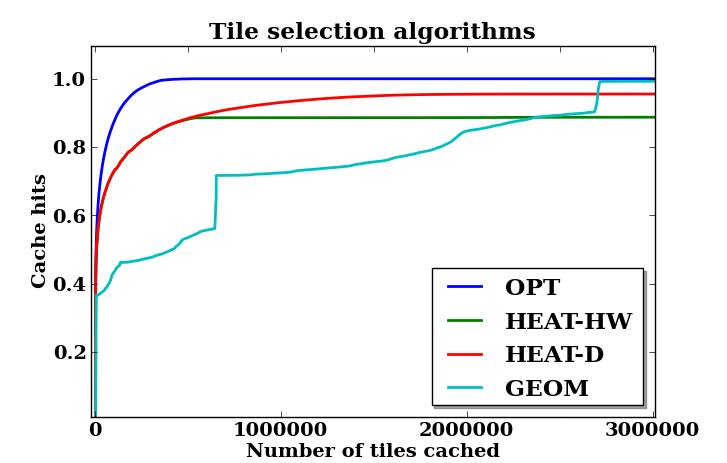
\includegraphics[scale=0.4]{figs-tileheat/results_closeup2.png}
\caption{The performance of tile selection algorithms for the first 3 million tiles selected, using three days of training data. The result is averaged over several runs using different data sets.}
\label{fig:results}
\end{figure*}

In Figure \ref{fig:results}, we show the average hit ratios obtained by the algorithms we have developed for TileHeat, using the datasets described in Section \ref{sec:datasets}. 
The figure shows the hit ratio of the first three million tiles that are selected by the algorithms. A full materialization contains more than ten million tiles. OPT, however, has a $100\%$ hit ratio after selecting 500,000 tiles. 

%OPT has a $100\%$ hit ratio after selecting 500,000 tiles.  %We also compare our algorithms against GEOM, which is the tile selection algorithm currently used by KMS.
As mentioned previously, the throughput of materializing tiles has been measured by KMS to be $58$ tiles per second on their infrastructure. A time window of $7.2$ hours fits inside the low load time period from $10$ PM to $6$ AM. During this window, we can compute $1.5$ million tiles. Within this tile budget, our best algorithm, HEAT-D, achieves a hit ratio of $95\%$. GEOM achieves a hit ratio of $76\%$ within the same tile budget. The hit ratio of HEAT-D is thus $25\%$ better than GEOM for this tile budget.

In general, we see that our algorithms rise significantly faster towards high hit ratios for small sets of tiles, e.g., in the 500,000 tile range. It is also clear that HEAT-D outperforms HEAT-HW after 500,000 tiles, and overall dominates HEAT-HW. This is because HEAT-D ranks more tiles than HEAT-HW, i.e., by ranking tiles that are not requested in the training workloads. We conclude that the additional tiles boost the hit ratio significantly, which confirms our hypothesis that tiles that are near to each other have similar access frequencies.

At around $2.6$ million tiles, GEOM overtakes HEAT-D, and becomes optimal. A peculiar effect of GEOM is a staircase effect that can be seen in Figure~\ref{fig:results}. We believe that this is an artifact of the way GEOM selects tiles --- selecting row-by-row the tiles that intersect the geometries provided. At certain latitudes, the rows cross over highly popular areas like the capital of Denmark, Copenhagen. The city of Copenhagen is clearly visible as a high-heat, dark area in the right side of each of the heatmaps shown in Figure~\ref{fig:heatmaps}. There are several steps in the staircase, as this effect is repeated at higher resolutions.

\section{Related work}
\label{sec:tileheat:related:work}

Caching of dynamic web content has been extensively studied in a number of contexts~\cite{DDT+01:DynamicContentAcceleration,GMA+08:Ferdinand,GLR05:GoodEnough,LGZ04:MTCache,LKM+02:DBCache,Moh01:WebCaching}. A major issue investigated by these proposals is the policy used to keep the cache up-to-date. 
For example, Guo et al.~\cite{GLR05:GoodEnough} propose a set of declarative constraints that specify presence,  consistency, completeness, and currency of cached content. 
Garrod et al.~\cite{GMA+08:Ferdinand} explore how to take advantage of multiple cache servers while maintaining consistency. In contrast, our workload analysis shows that the main challenge for a geographical web service is the computational expense of the refresh procedure of the tile cache, rather than the freshness of relatively slowly updated map data. In this sense, our approach can be seen as similar to periodically refreshing a materialized view. This  ``view'' delivers the tile pyramid based on the underlying geographical data; however, it is both spatial and includes external user-defined functions to compute tile content. While similar in spirit to the materialized-view approach of MTCache~\cite{LGZ04:MTCache}, the additional complexities of our domain render the problem harder in several ways: First, not all of the view definition is available to the system, making it more difficult to predict which tiles are affected by which data and recompute selectively. Second, only portions of the view are of interest to end users, due to skew in access patterns, and it is not obvious how to define which portions are interesting ahead of time. Third, computation of tiles is a very resource-intensive user-defined function, making even a partial refresh of the spatial cache costly.  
 
Our work can also be seen as a self-tuning approach to managing a tile web cache~\cite{CN07:SelfTuning10YrPaper}. Similarly to online self-tuning approaches, such as COLT~\cite{SAMP07:COLT} and the seminal COMFORT~\cite{WHMZ94:COMFORT} project, TileHeat operates on a feedback loop, collecting workload characteristics, performing reasoning for choosing a new system configuration, and introducing configuration changes as necessary. However, our work differs in both the characterization of the problem as well as in the design choices we make for each step of our feedback loop. 
In particular, our choices are motivated by a careful analysis of the production log of a country-wide geographical web service. 
%We derive several conclusions from the analysis: 1) The access patterns of the rendering service exhibit high regularity, with low activity off day hours; 2) Access patterns can be largely inferred based on historical data, 3) The cost for materialization of tiles for caching is significant, and consequently services with moderate update rates -- such as geographical web services -- can dramatically profit from a selective cache.  

Adaptive algorithms have been studied for the classic buffer cache replacement problem, including 2Q~\cite{JS94:2Q}, ARC~\cite{MM03:ARC}, and LRU-K~\cite{OOW93:LRU-K}. Our work, however, is focused on the different scenario of spatial web caching, in which tiles are materialized in advance of processing the workload.
% Unlike previous caching algorithms, our approach takes advantage of the capability to observe the workload for a given time period, and uses the collected data to materialize a spatial cache for the next period.  
As in semantic caching~\cite{DFJ+96:SemanticCaching}, we exploit application characteristics to decide what data to cache and update. In contrast to semantic caching, we exploit spatial properties for higher web cache hit ratios, such as with our heat dissipation method. 
	
The basic idea of using heat to measure popularity of data items arises naturally in applications with skewed access patterns. For example, Scheuermann et al.~\cite{SWZ93:DiskCooling} propose schemes for data placement and adaptive load balancing that "cool" disks by redistributing file fragments. In spatial services more specifically, many researchers have observed that there is a strong skew in the access frequencies of tiles, and that this skew follows a power law~\cite{fisher07,LGXF12:SpatialPrefetching,talagala00}. Li et al.~\cite{LGXF12:SpatialPrefetching} exploit skew to create a pre-fetching model of spatial tiles, with focus on predicting short-term user navigation. Their work is based on a substantial body of related short-term prediction approaches~\cite{KKK01:Prefetching,KKK01:Prefetching2,LKK+02:Prefetching}. These methods are optimized for pre-fetching  tiles seconds before they are requested by a user. The amount of pre-fetching done during a time period is thus proportional to the load. As we have observed, load and latency are proportional, which means that pre-fetching in real time does little to alleviate load peaks. To reduce the high latency caused by load peaks, we instead pre-compute tiles during periods of low load. To achieve this, we develop methods that do not rely on the input of individual users browsing a map in real time. 
%In contrast, we look at the problem of pre-computing a large set of tiles that comprise a production-grade spatial web cache. 

As discussed in Section~\ref{sec:existing:methods}, Quinn and Gahegan~\cite{quinn10} suggest using certain classes of base objects, such as roads and coastlines, as predictors of where users will look at a map. However, as observed in Fisher's study of Microsoft Hotmap~\cite{fisher07}, real-world workloads can contradict models of rational user behavior, exclusively focused on a fixed set of rules. An example given by Fisher~\cite{fisher07} was a banner ad that caused frequent requests for ``empty'' parts of the Pacific Ocean. Based on such observations of real-life events, Fisher develops a multi-scale descriptive model that quantifies web map usage based on a heatmap. Their study supports our observation that anomalous patterns may be transient in time, but partially detectable from a training data set. In contrast to Fisher, however, we exploit this insight to propose multiple strategies to keep hit ratios on a spatial web cache high, while at the same time drastically reducing resource consumption during recomputation of tiles. 

\section{Conclusion}
% What we did
In this work, we propose and evaluate the use of heatmaps to analyze the request log for a geospatial service as well as to improve the creation time of a tile cache for this service. 
As we have observed, heatmaps can be made predictive and aid in selecting a set of high traffic tiles. We applied our techniques to the request log of a production system and showed that substantial improvements over an existing method were attained. In particular, using our HEAT-D algorithm to compute a tile cache yields a $25\%$ improvement in the hit ratio for a reasonable time window of materialization. HEAT-D accurately predicts the popularity of tiles that are not requested in the training data by employing a heat diffusion process. 

% Future work
While our results improve on existing methods, for future work we plan to do a more thorough exploration of the parameter space of the algorithms HEAT-HW and HEAT-D to investigate if further improvements could be achieved. In addition, we plan to work on efficient methods for materializing the tiles selected by our algorithms as well as use the trend information from HEAT-HW to build a distributed cache that adapts to sudden spikes in load. 
%Exploring efficient methods of materializing the tiles, given a plan computed by TileHeat, would bring the work full circle. 
Finally, deploying TileHeat in a production environment and measuring the effect on latency remains as an important direction of future work.


\chapter{Conclusion}
\label{chapter:conclusion}

\pitfall{\emph{I Am Utterly Perfect:} No work is perfect. An explicit discussion of the limitations of your work strengthens, rahter than weakens, your paper. Papers without a discussion of limitations, weaknesses, and implications feel unfinished or preliminary. For instance, how large of a dataset can your system handle? Can you categorize the kinds of datasets for which your technique is suitable and those for which it is not -- Tamara Munzner.

\emph{Discuss:} unsupported data types, e.g. text, trees, and graphs; unsupported operators, e.g. multi-scale aggregation and multi-scale displacement; limitations in data size, e.g. explain that while results are shown for Postgres, other and more scalable databases could be used.}


\bibliographystyle{plain}
\bibliography{thesis}
                             % Sample .bib file with references that match those in
                             % the 'Specifications Document (V1.5)' as well containing
                             % 'legacy' bibs and bibs with 'alternate codings'.
                             % Gerry Murray - March 2012



\end{document}  

